% Options for packages loaded elsewhere
\PassOptionsToPackage{unicode}{hyperref}
\PassOptionsToPackage{hyphens}{url}
%
\documentclass[
]{article}
\usepackage{amsmath,amssymb}
\usepackage{lmodern}
\usepackage{ifxetex,ifluatex}
\ifnum 0\ifxetex 1\fi\ifluatex 1\fi=0 % if pdftex
  \usepackage[T1]{fontenc}
  \usepackage[utf8]{inputenc}
  \usepackage{textcomp} % provide euro and other symbols
\else % if luatex or xetex
  \usepackage{unicode-math}
  \defaultfontfeatures{Scale=MatchLowercase}
  \defaultfontfeatures[\rmfamily]{Ligatures=TeX,Scale=1}
\fi
% Use upquote if available, for straight quotes in verbatim environments
\IfFileExists{upquote.sty}{\usepackage{upquote}}{}
\IfFileExists{microtype.sty}{% use microtype if available
  \usepackage[]{microtype}
  \UseMicrotypeSet[protrusion]{basicmath} % disable protrusion for tt fonts
}{}
\makeatletter
\@ifundefined{KOMAClassName}{% if non-KOMA class
  \IfFileExists{parskip.sty}{%
    \usepackage{parskip}
  }{% else
    \setlength{\parindent}{0pt}
    \setlength{\parskip}{6pt plus 2pt minus 1pt}}
}{% if KOMA class
  \KOMAoptions{parskip=half}}
\makeatother
\usepackage{xcolor}
\IfFileExists{xurl.sty}{\usepackage{xurl}}{} % add URL line breaks if available
\IfFileExists{bookmark.sty}{\usepackage{bookmark}}{\usepackage{hyperref}}
\hypersetup{
  pdftitle={Questionnaires data},
  pdfauthor={Corrado Caudek},
  hidelinks,
  pdfcreator={LaTeX via pandoc}}
\urlstyle{same} % disable monospaced font for URLs
\usepackage[margin=1in]{geometry}
\usepackage{color}
\usepackage{fancyvrb}
\newcommand{\VerbBar}{|}
\newcommand{\VERB}{\Verb[commandchars=\\\{\}]}
\DefineVerbatimEnvironment{Highlighting}{Verbatim}{commandchars=\\\{\}}
% Add ',fontsize=\small' for more characters per line
\usepackage{framed}
\definecolor{shadecolor}{RGB}{248,248,248}
\newenvironment{Shaded}{\begin{snugshade}}{\end{snugshade}}
\newcommand{\AlertTok}[1]{\textcolor[rgb]{0.94,0.16,0.16}{#1}}
\newcommand{\AnnotationTok}[1]{\textcolor[rgb]{0.56,0.35,0.01}{\textbf{\textit{#1}}}}
\newcommand{\AttributeTok}[1]{\textcolor[rgb]{0.77,0.63,0.00}{#1}}
\newcommand{\BaseNTok}[1]{\textcolor[rgb]{0.00,0.00,0.81}{#1}}
\newcommand{\BuiltInTok}[1]{#1}
\newcommand{\CharTok}[1]{\textcolor[rgb]{0.31,0.60,0.02}{#1}}
\newcommand{\CommentTok}[1]{\textcolor[rgb]{0.56,0.35,0.01}{\textit{#1}}}
\newcommand{\CommentVarTok}[1]{\textcolor[rgb]{0.56,0.35,0.01}{\textbf{\textit{#1}}}}
\newcommand{\ConstantTok}[1]{\textcolor[rgb]{0.00,0.00,0.00}{#1}}
\newcommand{\ControlFlowTok}[1]{\textcolor[rgb]{0.13,0.29,0.53}{\textbf{#1}}}
\newcommand{\DataTypeTok}[1]{\textcolor[rgb]{0.13,0.29,0.53}{#1}}
\newcommand{\DecValTok}[1]{\textcolor[rgb]{0.00,0.00,0.81}{#1}}
\newcommand{\DocumentationTok}[1]{\textcolor[rgb]{0.56,0.35,0.01}{\textbf{\textit{#1}}}}
\newcommand{\ErrorTok}[1]{\textcolor[rgb]{0.64,0.00,0.00}{\textbf{#1}}}
\newcommand{\ExtensionTok}[1]{#1}
\newcommand{\FloatTok}[1]{\textcolor[rgb]{0.00,0.00,0.81}{#1}}
\newcommand{\FunctionTok}[1]{\textcolor[rgb]{0.00,0.00,0.00}{#1}}
\newcommand{\ImportTok}[1]{#1}
\newcommand{\InformationTok}[1]{\textcolor[rgb]{0.56,0.35,0.01}{\textbf{\textit{#1}}}}
\newcommand{\KeywordTok}[1]{\textcolor[rgb]{0.13,0.29,0.53}{\textbf{#1}}}
\newcommand{\NormalTok}[1]{#1}
\newcommand{\OperatorTok}[1]{\textcolor[rgb]{0.81,0.36,0.00}{\textbf{#1}}}
\newcommand{\OtherTok}[1]{\textcolor[rgb]{0.56,0.35,0.01}{#1}}
\newcommand{\PreprocessorTok}[1]{\textcolor[rgb]{0.56,0.35,0.01}{\textit{#1}}}
\newcommand{\RegionMarkerTok}[1]{#1}
\newcommand{\SpecialCharTok}[1]{\textcolor[rgb]{0.00,0.00,0.00}{#1}}
\newcommand{\SpecialStringTok}[1]{\textcolor[rgb]{0.31,0.60,0.02}{#1}}
\newcommand{\StringTok}[1]{\textcolor[rgb]{0.31,0.60,0.02}{#1}}
\newcommand{\VariableTok}[1]{\textcolor[rgb]{0.00,0.00,0.00}{#1}}
\newcommand{\VerbatimStringTok}[1]{\textcolor[rgb]{0.31,0.60,0.02}{#1}}
\newcommand{\WarningTok}[1]{\textcolor[rgb]{0.56,0.35,0.01}{\textbf{\textit{#1}}}}
\usepackage{graphicx}
\makeatletter
\def\maxwidth{\ifdim\Gin@nat@width>\linewidth\linewidth\else\Gin@nat@width\fi}
\def\maxheight{\ifdim\Gin@nat@height>\textheight\textheight\else\Gin@nat@height\fi}
\makeatother
% Scale images if necessary, so that they will not overflow the page
% margins by default, and it is still possible to overwrite the defaults
% using explicit options in \includegraphics[width, height, ...]{}
\setkeys{Gin}{width=\maxwidth,height=\maxheight,keepaspectratio}
% Set default figure placement to htbp
\makeatletter
\def\fps@figure{htbp}
\makeatother
\setlength{\emergencystretch}{3em} % prevent overfull lines
\providecommand{\tightlist}{%
  \setlength{\itemsep}{0pt}\setlength{\parskip}{0pt}}
\setcounter{secnumdepth}{-\maxdimen} % remove section numbering
\ifluatex
  \usepackage{selnolig}  % disable illegal ligatures
\fi

\title{Questionnaires data}
\author{\href{https://ccaudek.github.io/}{Corrado Caudek}}
\date{First version Wed Jun 9 14:20:42 2021. Last modified 2021-06-16}

\begin{document}
\maketitle

\begin{Shaded}
\begin{Highlighting}[]
\FunctionTok{library}\NormalTok{(}\StringTok{"here"}\NormalTok{)}
\end{Highlighting}
\end{Shaded}

\begin{verbatim}
## here() starts at /Users/corrado/Documents/papers/ED_patients
\end{verbatim}

\begin{Shaded}
\begin{Highlighting}[]
\FunctionTok{library}\NormalTok{(}\StringTok{"tidyverse"}\NormalTok{)}
\end{Highlighting}
\end{Shaded}

\begin{verbatim}
## -- Attaching packages --------------------------------------- tidyverse 1.3.1 --
\end{verbatim}

\begin{verbatim}
## v ggplot2 3.3.3     v purrr   0.3.4
## v tibble  3.1.2     v dplyr   1.0.6
## v tidyr   1.1.3     v stringr 1.4.0
## v readr   1.4.0     v forcats 0.5.1
\end{verbatim}

\begin{verbatim}
## -- Conflicts ------------------------------------------ tidyverse_conflicts() --
## x dplyr::filter() masks stats::filter()
## x dplyr::lag()    masks stats::lag()
\end{verbatim}

\begin{Shaded}
\begin{Highlighting}[]
\FunctionTok{library}\NormalTok{(}\StringTok{"forcats"}\NormalTok{)}
\FunctionTok{library}\NormalTok{(}\StringTok{"readxl"}\NormalTok{)}
\FunctionTok{library}\NormalTok{(}\StringTok{"pROC"}\NormalTok{)}
\end{Highlighting}
\end{Shaded}

\begin{verbatim}
## Type 'citation("pROC")' for a citation.
\end{verbatim}

\begin{verbatim}
## 
## Caricamento pacchetto: 'pROC'
\end{verbatim}

\begin{verbatim}
## I seguenti oggetti sono mascherati da 'package:stats':
## 
##     cov, smooth, var
\end{verbatim}

\begin{Shaded}
\begin{Highlighting}[]
\FunctionTok{library}\NormalTok{(}\StringTok{"brms"}\NormalTok{)}
\end{Highlighting}
\end{Shaded}

\begin{verbatim}
## Caricamento del pacchetto richiesto: Rcpp
\end{verbatim}

\begin{verbatim}
## Loading 'brms' package (version 2.15.0). Useful instructions
## can be found by typing help('brms'). A more detailed introduction
## to the package is available through vignette('brms_overview').
\end{verbatim}

\begin{verbatim}
## 
## Caricamento pacchetto: 'brms'
\end{verbatim}

\begin{verbatim}
## Il seguente oggetto è mascherato da 'package:stats':
## 
##     ar
\end{verbatim}

\begin{Shaded}
\begin{Highlighting}[]
\FunctionTok{library}\NormalTok{(}\StringTok{"cmdstanr"}\NormalTok{)}
\end{Highlighting}
\end{Shaded}

\begin{verbatim}
## This is cmdstanr version 0.4.0.9000
\end{verbatim}

\begin{verbatim}
## - Online documentation and vignettes at mc-stan.org/cmdstanr
\end{verbatim}

\begin{verbatim}
## - Use set_cmdstan_path() to set the path to CmdStan
\end{verbatim}

\begin{verbatim}
## - Use install_cmdstan() to install CmdStan
\end{verbatim}

\begin{Shaded}
\begin{Highlighting}[]
\FunctionTok{set\_cmdstan\_path}\NormalTok{(}\StringTok{"/Users/corrado/cmdstan"}\NormalTok{)}
\end{Highlighting}
\end{Shaded}

\begin{verbatim}
## CmdStan path set to: /Users/corrado/cmdstan
\end{verbatim}

\begin{Shaded}
\begin{Highlighting}[]
\FunctionTok{library}\NormalTok{(}\StringTok{"ROCR"}\NormalTok{)}
\FunctionTok{library}\NormalTok{(}\StringTok{"tidybayes"}\NormalTok{)}
\end{Highlighting}
\end{Shaded}

\begin{verbatim}
## 
## Caricamento pacchetto: 'tidybayes'
\end{verbatim}

\begin{verbatim}
## I seguenti oggetti sono mascherati da 'package:brms':
## 
##     dstudent_t, pstudent_t, qstudent_t, rstudent_t
\end{verbatim}

\begin{Shaded}
\begin{Highlighting}[]
\FunctionTok{source}\NormalTok{(here}\SpecialCharTok{::}\FunctionTok{here}\NormalTok{(}\StringTok{"lib"}\NormalTok{, }\StringTok{"ed\_fnc.R"}\NormalTok{))}


\CommentTok{\# read questionnaries data}
\NormalTok{patients\_codes }\OtherTok{\textless{}{-}} \FunctionTok{get\_patients\_codes}\NormalTok{() }

\CommentTok{\# read PRL params and quest data}
\NormalTok{quest\_data }\OtherTok{\textless{}{-}} \FunctionTok{readRDS}\NormalTok{(}
  \FunctionTok{here}\NormalTok{(}\StringTok{"data"}\NormalTok{, }\StringTok{"processed"}\NormalTok{, }\StringTok{"prl"}\NormalTok{, }\StringTok{"prl\_and\_quest"}\NormalTok{, }
       \StringTok{"prl\_params\_and\_quest\_data.rds"}\NormalTok{)}
\NormalTok{)}

\NormalTok{quest\_data}\SpecialCharTok{$}\NormalTok{eat26\_tot }\OtherTok{\textless{}{-}}\NormalTok{ quest\_data}\SpecialCharTok{$}\NormalTok{dieting }\SpecialCharTok{+}\NormalTok{ quest\_data}\SpecialCharTok{$}\NormalTok{bulimia }\SpecialCharTok{+}\NormalTok{ quest\_data}\SpecialCharTok{$}\NormalTok{oral\_control}

\NormalTok{quest\_data }\SpecialCharTok{\%\textgreater{}\%} 
  \FunctionTok{group\_by}\NormalTok{(group) }\SpecialCharTok{\%\textgreater{}\%} 
  \FunctionTok{summarise}\NormalTok{(}
    \AttributeTok{avg\_eat26\_tot =} \FunctionTok{median}\NormalTok{(eat26\_tot, }\AttributeTok{na.rm =} \ConstantTok{TRUE}\NormalTok{), }
    \AttributeTok{avg\_eat26\_bu  =} \FunctionTok{median}\NormalTok{(bulimia, }\AttributeTok{na.rm =} \ConstantTok{TRUE}\NormalTok{), }
    \AttributeTok{avg\_eat26\_di  =} \FunctionTok{median}\NormalTok{(dieting, }\AttributeTok{na.rm =} \ConstantTok{TRUE}\NormalTok{), }
    \AttributeTok{avg\_eat26\_oc  =} \FunctionTok{median}\NormalTok{(oral\_control, }\AttributeTok{na.rm =} \ConstantTok{TRUE}\NormalTok{), }
    \AttributeTok{n =} \FunctionTok{n}\NormalTok{()}
\NormalTok{  )}
\end{Highlighting}
\end{Shaded}

\begin{verbatim}
## # A tibble: 3 x 6
##   group   avg_eat26_tot avg_eat26_bu avg_eat26_di avg_eat26_oc     n
##   <chr>           <dbl>        <dbl>        <dbl>        <dbl> <int>
## 1 at_risk            29            9           17          2.5    34
## 2 control             6            3            2          0     246
## 3 patient            39           11           22          8      25
\end{verbatim}

\begin{Shaded}
\begin{Highlighting}[]
\NormalTok{quest\_data }\SpecialCharTok{\%\textgreater{}\%} 
  \FunctionTok{group\_by}\NormalTok{(group) }\SpecialCharTok{\%\textgreater{}\%} 
  \FunctionTok{summarise}\NormalTok{(}
    \AttributeTok{avg\_dass\_a =} \FunctionTok{median}\NormalTok{(dass21\_anxiety, }\AttributeTok{na.rm =} \ConstantTok{TRUE}\NormalTok{), }
    \AttributeTok{avg\_dass\_s  =} \FunctionTok{median}\NormalTok{(dass21\_stress, }\AttributeTok{na.rm =} \ConstantTok{TRUE}\NormalTok{), }
    \AttributeTok{avg\_dass\_d  =} \FunctionTok{median}\NormalTok{(dass21\_dep, }\AttributeTok{na.rm =} \ConstantTok{TRUE}\NormalTok{),}
    \AttributeTok{n =} \FunctionTok{n}\NormalTok{()}
\NormalTok{  )}
\end{Highlighting}
\end{Shaded}

\begin{verbatim}
## # A tibble: 3 x 5
##   group   avg_dass_a avg_dass_s avg_dass_d     n
##   <chr>        <dbl>      <dbl>      <dbl> <int>
## 1 at_risk        7.5         13         10    34
## 2 control        4            9          6   246
## 3 patient        8           13         11    25
\end{verbatim}

\begin{Shaded}
\begin{Highlighting}[]
\NormalTok{quest\_data }\SpecialCharTok{\%\textgreater{}\%} 
  \FunctionTok{group\_by}\NormalTok{(group) }\SpecialCharTok{\%\textgreater{}\%} 
  \FunctionTok{summarise}\NormalTok{(}
    \AttributeTok{avg\_sias =} \FunctionTok{median}\NormalTok{(sias, }\AttributeTok{na.rm =} \ConstantTok{TRUE}\NormalTok{), }
    \AttributeTok{avg\_orto  =} \FunctionTok{median}\NormalTok{(orto\_tot, }\AttributeTok{na.rm =} \ConstantTok{TRUE}\NormalTok{), }
    \AttributeTok{avg\_ros  =} \FunctionTok{median}\NormalTok{(ros\_tot, }\AttributeTok{na.rm =} \ConstantTok{TRUE}\NormalTok{),}
    \AttributeTok{avg\_bsq14  =} \FunctionTok{median}\NormalTok{(bsq14\_tot, }\AttributeTok{na.rm =} \ConstantTok{TRUE}\NormalTok{),}
    \AttributeTok{n =} \FunctionTok{n}\NormalTok{()}
\NormalTok{  )}
\end{Highlighting}
\end{Shaded}

\begin{verbatim}
## # A tibble: 3 x 6
##   group   avg_sias avg_orto avg_ros avg_bsq14     n
##   <chr>      <dbl>    <dbl>   <dbl>     <dbl> <int>
## 1 at_risk     37.5       15    26.5      65.5    34
## 2 control     26         21    21        36     246
## 3 patient     35         13    26        63      25
\end{verbatim}

\begin{Shaded}
\begin{Highlighting}[]
\NormalTok{quest\_data }\SpecialCharTok{\%\textgreater{}\%} 
  \FunctionTok{group\_by}\NormalTok{(group) }\SpecialCharTok{\%\textgreater{}\%} 
  \FunctionTok{summarise}\NormalTok{(}
    \AttributeTok{avg\_ps =} \FunctionTok{median}\NormalTok{(mps\_ps, }\AttributeTok{na.rm =} \ConstantTok{TRUE}\NormalTok{), }
    \AttributeTok{avg\_o  =} \FunctionTok{median}\NormalTok{(mps\_o, }\AttributeTok{na.rm =} \ConstantTok{TRUE}\NormalTok{), }
    \AttributeTok{avg\_cmd  =} \FunctionTok{median}\NormalTok{(mps\_cmd, }\AttributeTok{na.rm =} \ConstantTok{TRUE}\NormalTok{),}
    \AttributeTok{avg\_pepc  =} \FunctionTok{median}\NormalTok{(mps\_pepc, }\AttributeTok{na.rm =} \ConstantTok{TRUE}\NormalTok{),}
    \AttributeTok{n =} \FunctionTok{n}\NormalTok{()}
\NormalTok{  )}
\end{Highlighting}
\end{Shaded}

\begin{verbatim}
## # A tibble: 3 x 6
##   group   avg_ps avg_o avg_cmd avg_pepc     n
##   <chr>    <dbl> <dbl>   <dbl>    <dbl> <int>
## 1 at_risk     25  22.5      51       21    34
## 2 control     21  22        42       18   246
## 3 patient     25  24        48       22    25
\end{verbatim}

\begin{Shaded}
\begin{Highlighting}[]
\NormalTok{subj\_info }\OtherTok{\textless{}{-}} \FunctionTok{get\_subj\_info}\NormalTok{()}

\NormalTok{quest\_data2 }\OtherTok{\textless{}{-}} \FunctionTok{left\_join}\NormalTok{(quest\_data, subj\_info, }\AttributeTok{by =} \StringTok{"subj\_code"}\NormalTok{)}
\NormalTok{quest\_data2}\SpecialCharTok{$}\NormalTok{height  }
\end{Highlighting}
\end{Shaded}

\begin{verbatim}
##   [1] 155.0 168.0 176.0 156.0    NA    NA 169.0 165.0 162.0 169.0 170.0    NA
##  [13] 168.0    NA    NA 165.0    NA    NA    NA 168.0 170.0 163.0 158.0    NA
##  [25] 164.0 160.0    NA 160.0    NA 165.0 170.0    NA    NA 148.0 176.0    NA
##  [37] 165.0    NA 184.0 168.0 170.0 165.0 168.0 163.0 160.0 163.0 167.0 167.0
##  [49] 168.0 162.0 165.0 160.0 159.0 164.0 160.0    NA 162.0 162.0    NA 162.0
##  [61] 156.0 160.0 165.0 165.0 174.0 165.0 169.0 150.0 167.0 176.0 160.0 165.0
##  [73] 170.0 165.0 155.0 164.0 169.0 169.0 169.0 162.0 155.0 170.0    NA 168.0
##  [85] 174.0    NA 160.0 168.0 168.0 155.0 158.0 170.0 167.0 162.0 164.0 160.0
##  [97] 167.0 170.0 178.0 171.0 168.0 160.0 170.0 168.0 160.0 164.0    NA 160.0
## [109] 164.0 160.0 160.0 188.0 171.0    NA 158.0 170.0 175.0 177.0 165.0    NA
## [121] 174.0 160.0 165.0 160.0    NA 158.0 163.0 163.0 171.0 160.0 162.0 176.0
## [133] 182.0 160.0 167.0 170.0 179.0 170.0 161.0 163.0 160.0 163.0 174.0 154.0
## [145] 173.0 163.0 173.0 170.0 166.0 183.0 170.0 165.0 163.0 163.0 158.0 170.0
## [157] 153.0    NA 175.0 163.0 180.0 180.0 169.0 174.0 187.0 169.0 165.0 169.0
## [169] 169.0 163.0 165.0 175.0 160.0 160.0 163.0 164.0 175.0 163.0 160.0 165.0
## [181] 165.0 168.0 170.0 174.0 171.0 167.0 180.0 167.0 165.0 168.0 175.0 175.0
## [193] 175.0 180.0 183.0 170.0 166.0 168.0 172.0 175.0 173.0 163.0 169.0 169.0
## [205] 164.0 167.0 167.0 167.0 167.0 167.0 167.0 180.0    NA 156.0 160.0 158.0
## [217] 165.0 155.0 160.0    NA 180.0 158.0 170.0 161.0 167.0 165.0    NA 169.0
## [229] 170.0 163.0    NA 165.0 170.0 158.0 158.0 164.0 180.0 168.0 173.0 150.0
## [241] 164.0    NA 177.0 165.0 162.0 178.0 171.0 165.0 155.0 158.0 160.0 166.0
## [253] 165.0 170.0 170.0 165.0 167.0 158.0    NA 159.0    NA 162.0 165.0 151.0
## [265] 170.0    NA    NA 160.0 160.0 160.0 177.0 173.0 180.0 154.0 165.0 164.0
## [277] 170.0 158.0 165.0 169.0 163.0 170.0 169.0 165.0 165.0 165.0 167.0 187.0
## [289] 187.0 160.0 193.0 170.0 174.0 160.0 157.0 170.0    NA 170.0 158.0 156.0
## [301] 171.5    NA 170.0 170.0 180.0 170.0    NA 162.0 162.0 160.0 173.0 158.0
## [313] 187.0 162.0 174.0 165.0 171.0 170.0 167.0    NA    NA 175.0 166.0 176.0
## [325]    NA 172.0 155.0
\end{verbatim}

\begin{Shaded}
\begin{Highlighting}[]
\NormalTok{quest\_data2}\SpecialCharTok{$}\NormalTok{present\_weight}
\end{Highlighting}
\end{Shaded}

\begin{verbatim}
##   [1]  40.00 116.00  52.00  38.00     NA     NA  47.00 100.00  80.00  67.00
##  [11]  55.40     NA  45.00     NA     NA  50.00     NA     NA     NA  47.00
##  [21]  74.00  48.00  40.00     NA  75.00  57.00     NA  50.00     NA  42.00
##  [31]  52.00     NA     NA     NA  53.00     NA  83.00     NA  82.00  56.00
##  [41]  47.00 100.00  52.00  54.00  56.00  52.50  61.00  61.00  62.00  70.00
##  [51]  55.00  49.00  63.00  74.00  78.00     NA  52.00  52.00     NA  57.00
##  [61]  48.00  50.00  50.00  58.00  60.00  56.00  80.00  43.00  75.00  66.40
##  [71]  48.00  55.00  85.00  51.00  60.00  53.00  60.00  60.00  60.00  58.00
##  [81]  52.75  60.00     NA  54.00  82.00     NA  55.00  56.00  56.00  47.00
##  [91]  48.00  61.00  53.00  52.00  50.00  53.00  46.00  53.00  68.00  63.00
## [101]  60.00  64.50  65.00  60.00  56.00  52.00     NA  49.00  54.00  48.00
## [111]  49.00  65.00  56.00     NA  52.00  80.00  65.00  65.00  58.00     NA
## [121]  80.00  43.00  53.00  64.00     NA  60.00  57.00  50.00  68.00  80.00
## [131]  53.00  60.00  70.00  57.00  53.00  64.00  80.00  72.00  67.00  48.00
## [141]  55.00  55.00  71.00  51.00  48.00  52.00  45.00  62.00  56.00  90.00
## [151]  60.00  57.00  58.00  58.00  53.00  60.00  46.00     NA  64.00  52.00
## [161]  65.00  65.00  48.50  68.00  78.00  76.00  65.00  59.50  53.00  48.00
## [171]  57.00  65.00  60.00  60.00  50.00  48.00  72.00  52.00  51.00  49.00
## [181]  60.00  54.00  67.00 103.00  58.00  85.00  83.00  72.00  65.00  65.00
## [191]  55.00  55.00  55.00  77.00  66.00  60.00  56.00  47.00  59.00  50.00
## [201]  68.00  47.00  62.00  59.00  55.00  54.00  54.00  54.00  54.00  54.00
## [211]  54.00 100.00     NA  55.00  70.00  52.00  65.00  48.00  62.00     NA
## [221]  64.00  55.00  54.00  37.00  60.00  50.00     NA  60.00  73.00  52.00
## [231]     NA  65.00  55.00  53.00  55.00  84.00  90.00  70.00  68.00  53.00
## [241]  59.00     NA  78.00  53.00  55.00  60.00  58.00  60.00  57.00  55.00
## [251]  60.00  53.00 130.00  54.00  54.00  49.00  61.00  58.00     NA  61.00
## [261]     NA  51.00  67.00  48.00  80.00     NA     NA  45.00  45.00  45.00
## [271]  75.00  55.00  80.00  52.00  70.00  59.00  55.00  54.00  59.00  70.00
## [281]  60.00  63.00  76.00  55.00  55.00  57.00  62.00  72.00  72.00  51.70
## [291]  70.00  60.00  95.00  48.00  58.00  60.00     NA  84.70  48.00  47.00
## [301]  57.00     NA  70.00  51.00  77.00  61.00     NA  54.50  54.50  49.00
## [311]  68.00  52.00  88.00  62.00  56.00  54.00  69.00  55.00  61.00     NA
## [321]     NA  68.00  55.00  57.00     NA  62.00  48.00
\end{verbatim}

\begin{Shaded}
\begin{Highlighting}[]
\NormalTok{quest\_data2}\SpecialCharTok{$}\NormalTok{bmi }\OtherTok{\textless{}{-}}\NormalTok{ quest\_data2}\SpecialCharTok{$}\NormalTok{present\_weight }\SpecialCharTok{/}\NormalTok{ (quest\_data2}\SpecialCharTok{$}\NormalTok{height}\SpecialCharTok{/}\DecValTok{100}\NormalTok{)}\SpecialCharTok{\^{}}\DecValTok{2}
\FunctionTok{hist}\NormalTok{(quest\_data2}\SpecialCharTok{$}\NormalTok{bmi)}
\end{Highlighting}
\end{Shaded}

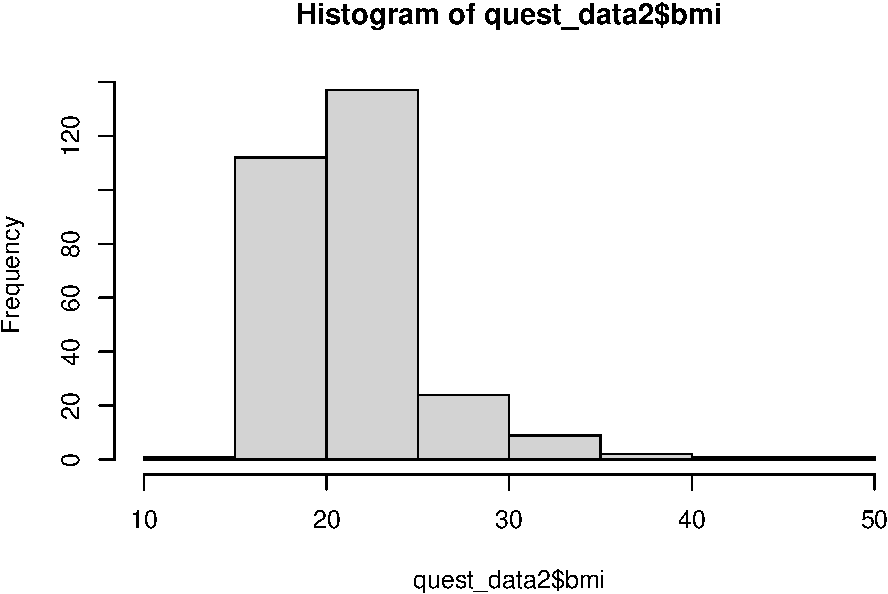
\includegraphics{050_quest_groups_files/figure-latex/unnamed-chunk-1-1.pdf}

\begin{Shaded}
\begin{Highlighting}[]
\CommentTok{\# sort(quest\_data2$bmi)}

\NormalTok{m1 }\OtherTok{\textless{}{-}} \FunctionTok{brm}\NormalTok{(}
\NormalTok{  bmi }\SpecialCharTok{\textasciitilde{}}\NormalTok{ age }\SpecialCharTok{+}\NormalTok{ sex }\SpecialCharTok{+}  
\NormalTok{       oral\_control }\SpecialCharTok{+}\NormalTok{ dieting }\SpecialCharTok{+}\NormalTok{ bulimia }\SpecialCharTok{+}
\NormalTok{       bsq14\_tot }\SpecialCharTok{+}\NormalTok{ ros\_tot }\SpecialCharTok{+}
\NormalTok{       dass21\_stress }\SpecialCharTok{+}\NormalTok{ dass21\_anxiety }\SpecialCharTok{+}\NormalTok{ dass21\_dep }\SpecialCharTok{+}
\NormalTok{       sias }\SpecialCharTok{+}\NormalTok{ mps\_ps }\SpecialCharTok{+}\NormalTok{ mps\_o }\SpecialCharTok{+}\NormalTok{ mps\_cmd }\SpecialCharTok{+}\NormalTok{ mps\_pepc }\SpecialCharTok{+}\NormalTok{ orto\_tot,}
  \AttributeTok{data =}\NormalTok{ quest\_data2, }
  \CommentTok{\# prior = prior\_ma,}
  \AttributeTok{family =} \FunctionTok{skew\_normal}\NormalTok{(),}
  \AttributeTok{control =} \FunctionTok{list}\NormalTok{(}\AttributeTok{adapt\_delta =} \FloatTok{0.98}\NormalTok{),}
  \AttributeTok{iter =} \DecValTok{4000}\NormalTok{,}
  \AttributeTok{cores =} \DecValTok{6}\NormalTok{,}
  \AttributeTok{backend =} \StringTok{"cmdstan"}
\NormalTok{)}
\end{Highlighting}
\end{Shaded}

\begin{verbatim}
## Warning: Rows containing NAs were excluded from the model.
\end{verbatim}

\begin{verbatim}
## Start sampling
\end{verbatim}

\begin{verbatim}
## Running MCMC with 4 chains, at most 6 in parallel...
\end{verbatim}

\begin{verbatim}
## Chain 1 Rejecting initial value:
\end{verbatim}

\begin{verbatim}
## Chain 1   Log probability evaluates to log(0), i.e. negative infinity.
\end{verbatim}

\begin{verbatim}
## Chain 1   Stan can't start sampling from this initial value.
\end{verbatim}

\begin{verbatim}
## Chain 1 Iteration:    1 / 4000 [  0%]  (Warmup)
\end{verbatim}

\begin{verbatim}
## Chain 2 Rejecting initial value:
\end{verbatim}

\begin{verbatim}
## Chain 2   Log probability evaluates to log(0), i.e. negative infinity.
\end{verbatim}

\begin{verbatim}
## Chain 2   Stan can't start sampling from this initial value.
\end{verbatim}

\begin{verbatim}
## Chain 2 Iteration:    1 / 4000 [  0%]  (Warmup) 
## Chain 3 Iteration:    1 / 4000 [  0%]  (Warmup) 
## Chain 4 Iteration:    1 / 4000 [  0%]  (Warmup) 
## Chain 3 Iteration:  100 / 4000 [  2%]  (Warmup) 
## Chain 1 Iteration:  100 / 4000 [  2%]  (Warmup) 
## Chain 2 Iteration:  100 / 4000 [  2%]  (Warmup) 
## Chain 3 Iteration:  200 / 4000 [  5%]  (Warmup) 
## Chain 1 Iteration:  200 / 4000 [  5%]  (Warmup) 
## Chain 1 Iteration:  300 / 4000 [  7%]  (Warmup) 
## Chain 2 Iteration:  200 / 4000 [  5%]  (Warmup) 
## Chain 3 Iteration:  300 / 4000 [  7%]  (Warmup) 
## Chain 4 Iteration:  100 / 4000 [  2%]  (Warmup) 
## Chain 1 Iteration:  400 / 4000 [ 10%]  (Warmup) 
## Chain 3 Iteration:  400 / 4000 [ 10%]  (Warmup) 
## Chain 4 Iteration:  200 / 4000 [  5%]  (Warmup) 
## Chain 1 Iteration:  500 / 4000 [ 12%]  (Warmup) 
## Chain 2 Iteration:  300 / 4000 [  7%]  (Warmup) 
## Chain 1 Iteration:  600 / 4000 [ 15%]  (Warmup) 
## Chain 2 Iteration:  400 / 4000 [ 10%]  (Warmup) 
## Chain 3 Iteration:  500 / 4000 [ 12%]  (Warmup) 
## Chain 4 Iteration:  300 / 4000 [  7%]  (Warmup) 
## Chain 1 Iteration:  700 / 4000 [ 17%]  (Warmup) 
## Chain 3 Iteration:  600 / 4000 [ 15%]  (Warmup) 
## Chain 4 Iteration:  400 / 4000 [ 10%]  (Warmup) 
## Chain 1 Iteration:  800 / 4000 [ 20%]  (Warmup) 
## Chain 2 Iteration:  500 / 4000 [ 12%]  (Warmup) 
## Chain 3 Iteration:  700 / 4000 [ 17%]  (Warmup) 
## Chain 4 Iteration:  500 / 4000 [ 12%]  (Warmup) 
## Chain 1 Iteration:  900 / 4000 [ 22%]  (Warmup) 
## Chain 2 Iteration:  600 / 4000 [ 15%]  (Warmup) 
## Chain 3 Iteration:  800 / 4000 [ 20%]  (Warmup) 
## Chain 4 Iteration:  600 / 4000 [ 15%]  (Warmup) 
## Chain 2 Iteration:  700 / 4000 [ 17%]  (Warmup) 
## Chain 3 Iteration:  900 / 4000 [ 22%]  (Warmup) 
## Chain 4 Iteration:  700 / 4000 [ 17%]  (Warmup) 
## Chain 1 Iteration: 1000 / 4000 [ 25%]  (Warmup) 
## Chain 3 Iteration: 1000 / 4000 [ 25%]  (Warmup) 
## Chain 1 Iteration: 1100 / 4000 [ 27%]  (Warmup) 
## Chain 2 Iteration:  800 / 4000 [ 20%]  (Warmup) 
## Chain 3 Iteration: 1100 / 4000 [ 27%]  (Warmup) 
## Chain 4 Iteration:  800 / 4000 [ 20%]  (Warmup) 
## Chain 1 Iteration: 1200 / 4000 [ 30%]  (Warmup) 
## Chain 4 Iteration:  900 / 4000 [ 22%]  (Warmup) 
## Chain 1 Iteration: 1300 / 4000 [ 32%]  (Warmup) 
## Chain 2 Iteration:  900 / 4000 [ 22%]  (Warmup) 
## Chain 3 Iteration: 1200 / 4000 [ 30%]  (Warmup) 
## Chain 4 Iteration: 1000 / 4000 [ 25%]  (Warmup) 
## Chain 1 Iteration: 1400 / 4000 [ 35%]  (Warmup) 
## Chain 2 Iteration: 1000 / 4000 [ 25%]  (Warmup) 
## Chain 3 Iteration: 1300 / 4000 [ 32%]  (Warmup) 
## Chain 4 Iteration: 1100 / 4000 [ 27%]  (Warmup) 
## Chain 2 Iteration: 1100 / 4000 [ 27%]  (Warmup) 
## Chain 3 Iteration: 1400 / 4000 [ 35%]  (Warmup) 
## Chain 4 Iteration: 1200 / 4000 [ 30%]  (Warmup) 
## Chain 1 Iteration: 1500 / 4000 [ 37%]  (Warmup) 
## Chain 2 Iteration: 1200 / 4000 [ 30%]  (Warmup) 
## Chain 3 Iteration: 1500 / 4000 [ 37%]  (Warmup) 
## Chain 4 Iteration: 1300 / 4000 [ 32%]  (Warmup) 
## Chain 1 Iteration: 1600 / 4000 [ 40%]  (Warmup) 
## Chain 2 Iteration: 1300 / 4000 [ 32%]  (Warmup) 
## Chain 3 Iteration: 1600 / 4000 [ 40%]  (Warmup) 
## Chain 4 Iteration: 1400 / 4000 [ 35%]  (Warmup) 
## Chain 1 Iteration: 1700 / 4000 [ 42%]  (Warmup) 
## Chain 2 Iteration: 1400 / 4000 [ 35%]  (Warmup) 
## Chain 3 Iteration: 1700 / 4000 [ 42%]  (Warmup) 
## Chain 4 Iteration: 1500 / 4000 [ 37%]  (Warmup) 
## Chain 1 Iteration: 1800 / 4000 [ 45%]  (Warmup) 
## Chain 2 Iteration: 1500 / 4000 [ 37%]  (Warmup) 
## Chain 3 Iteration: 1800 / 4000 [ 45%]  (Warmup) 
## Chain 1 Iteration: 1900 / 4000 [ 47%]  (Warmup) 
## Chain 2 Iteration: 1600 / 4000 [ 40%]  (Warmup) 
## Chain 3 Iteration: 1900 / 4000 [ 47%]  (Warmup) 
## Chain 4 Iteration: 1600 / 4000 [ 40%]  (Warmup) 
## Chain 2 Iteration: 1700 / 4000 [ 42%]  (Warmup) 
## Chain 4 Iteration: 1700 / 4000 [ 42%]  (Warmup) 
## Chain 1 Iteration: 2000 / 4000 [ 50%]  (Warmup) 
## Chain 1 Iteration: 2001 / 4000 [ 50%]  (Sampling) 
## Chain 2 Iteration: 1800 / 4000 [ 45%]  (Warmup) 
## Chain 4 Iteration: 1800 / 4000 [ 45%]  (Warmup) 
## Chain 1 Iteration: 2100 / 4000 [ 52%]  (Sampling) 
## Chain 2 Iteration: 1900 / 4000 [ 47%]  (Warmup) 
## Chain 3 Iteration: 2000 / 4000 [ 50%]  (Warmup) 
## Chain 3 Iteration: 2001 / 4000 [ 50%]  (Sampling) 
## Chain 4 Iteration: 1900 / 4000 [ 47%]  (Warmup) 
## Chain 2 Iteration: 2000 / 4000 [ 50%]  (Warmup) 
## Chain 2 Iteration: 2001 / 4000 [ 50%]  (Sampling) 
## Chain 3 Iteration: 2100 / 4000 [ 52%]  (Sampling) 
## Chain 1 Iteration: 2200 / 4000 [ 55%]  (Sampling) 
## Chain 2 Iteration: 2100 / 4000 [ 52%]  (Sampling) 
## Chain 4 Iteration: 2000 / 4000 [ 50%]  (Warmup) 
## Chain 4 Iteration: 2001 / 4000 [ 50%]  (Sampling) 
## Chain 1 Iteration: 2300 / 4000 [ 57%]  (Sampling) 
## Chain 3 Iteration: 2200 / 4000 [ 55%]  (Sampling) 
## Chain 4 Iteration: 2100 / 4000 [ 52%]  (Sampling) 
## Chain 1 Iteration: 2400 / 4000 [ 60%]  (Sampling) 
## Chain 2 Iteration: 2200 / 4000 [ 55%]  (Sampling) 
## Chain 3 Iteration: 2300 / 4000 [ 57%]  (Sampling) 
## Chain 2 Iteration: 2300 / 4000 [ 57%]  (Sampling) 
## Chain 4 Iteration: 2200 / 4000 [ 55%]  (Sampling) 
## Chain 1 Iteration: 2500 / 4000 [ 62%]  (Sampling) 
## Chain 2 Iteration: 2400 / 4000 [ 60%]  (Sampling) 
## Chain 3 Iteration: 2400 / 4000 [ 60%]  (Sampling) 
## Chain 4 Iteration: 2300 / 4000 [ 57%]  (Sampling) 
## Chain 1 Iteration: 2600 / 4000 [ 65%]  (Sampling) 
## Chain 3 Iteration: 2500 / 4000 [ 62%]  (Sampling) 
## Chain 1 Iteration: 2700 / 4000 [ 67%]  (Sampling) 
## Chain 2 Iteration: 2500 / 4000 [ 62%]  (Sampling) 
## Chain 4 Iteration: 2400 / 4000 [ 60%]  (Sampling) 
## Chain 2 Iteration: 2600 / 4000 [ 65%]  (Sampling) 
## Chain 3 Iteration: 2600 / 4000 [ 65%]  (Sampling) 
## Chain 4 Iteration: 2500 / 4000 [ 62%]  (Sampling) 
## Chain 1 Iteration: 2800 / 4000 [ 70%]  (Sampling) 
## Chain 2 Iteration: 2700 / 4000 [ 67%]  (Sampling) 
## Chain 3 Iteration: 2700 / 4000 [ 67%]  (Sampling) 
## Chain 1 Iteration: 2900 / 4000 [ 72%]  (Sampling) 
## Chain 2 Iteration: 2800 / 4000 [ 70%]  (Sampling) 
## Chain 4 Iteration: 2600 / 4000 [ 65%]  (Sampling) 
## Chain 1 Iteration: 3000 / 4000 [ 75%]  (Sampling) 
## Chain 3 Iteration: 2800 / 4000 [ 70%]  (Sampling) 
## Chain 4 Iteration: 2700 / 4000 [ 67%]  (Sampling) 
## Chain 2 Iteration: 2900 / 4000 [ 72%]  (Sampling) 
## Chain 1 Iteration: 3100 / 4000 [ 77%]  (Sampling) 
## Chain 2 Iteration: 3000 / 4000 [ 75%]  (Sampling) 
## Chain 3 Iteration: 2900 / 4000 [ 72%]  (Sampling) 
## Chain 4 Iteration: 2800 / 4000 [ 70%]  (Sampling) 
## Chain 1 Iteration: 3200 / 4000 [ 80%]  (Sampling) 
## Chain 2 Iteration: 3100 / 4000 [ 77%]  (Sampling) 
## Chain 3 Iteration: 3000 / 4000 [ 75%]  (Sampling) 
## Chain 4 Iteration: 2900 / 4000 [ 72%]  (Sampling) 
## Chain 1 Iteration: 3300 / 4000 [ 82%]  (Sampling) 
## Chain 2 Iteration: 3200 / 4000 [ 80%]  (Sampling) 
## Chain 4 Iteration: 3000 / 4000 [ 75%]  (Sampling) 
## Chain 3 Iteration: 3100 / 4000 [ 77%]  (Sampling) 
## Chain 1 Iteration: 3400 / 4000 [ 85%]  (Sampling) 
## Chain 2 Iteration: 3300 / 4000 [ 82%]  (Sampling) 
## Chain 3 Iteration: 3200 / 4000 [ 80%]  (Sampling) 
## Chain 4 Iteration: 3100 / 4000 [ 77%]  (Sampling) 
## Chain 1 Iteration: 3500 / 4000 [ 87%]  (Sampling) 
## Chain 2 Iteration: 3400 / 4000 [ 85%]  (Sampling) 
## Chain 4 Iteration: 3200 / 4000 [ 80%]  (Sampling) 
## Chain 2 Iteration: 3500 / 4000 [ 87%]  (Sampling) 
## Chain 3 Iteration: 3300 / 4000 [ 82%]  (Sampling) 
## Chain 1 Iteration: 3600 / 4000 [ 90%]  (Sampling) 
## Chain 3 Iteration: 3400 / 4000 [ 85%]  (Sampling) 
## Chain 4 Iteration: 3300 / 4000 [ 82%]  (Sampling) 
## Chain 1 Iteration: 3700 / 4000 [ 92%]  (Sampling) 
## Chain 2 Iteration: 3600 / 4000 [ 90%]  (Sampling) 
## Chain 4 Iteration: 3400 / 4000 [ 85%]  (Sampling) 
## Chain 1 Iteration: 3800 / 4000 [ 95%]  (Sampling) 
## Chain 2 Iteration: 3700 / 4000 [ 92%]  (Sampling) 
## Chain 3 Iteration: 3500 / 4000 [ 87%]  (Sampling) 
## Chain 2 Iteration: 3800 / 4000 [ 95%]  (Sampling) 
## Chain 4 Iteration: 3500 / 4000 [ 87%]  (Sampling) 
## Chain 1 Iteration: 3900 / 4000 [ 97%]  (Sampling) 
## Chain 2 Iteration: 3900 / 4000 [ 97%]  (Sampling) 
## Chain 3 Iteration: 3600 / 4000 [ 90%]  (Sampling) 
## Chain 4 Iteration: 3600 / 4000 [ 90%]  (Sampling) 
## Chain 1 Iteration: 4000 / 4000 [100%]  (Sampling) 
## Chain 3 Iteration: 3700 / 4000 [ 92%]  (Sampling) 
## Chain 1 finished in 5.6 seconds.
## Chain 2 Iteration: 4000 / 4000 [100%]  (Sampling) 
## Chain 4 Iteration: 3700 / 4000 [ 92%]  (Sampling) 
## Chain 2 finished in 5.7 seconds.
## Chain 3 Iteration: 3800 / 4000 [ 95%]  (Sampling) 
## Chain 4 Iteration: 3800 / 4000 [ 95%]  (Sampling) 
## Chain 3 Iteration: 3900 / 4000 [ 97%]  (Sampling) 
## Chain 4 Iteration: 3900 / 4000 [ 97%]  (Sampling) 
## Chain 3 Iteration: 4000 / 4000 [100%]  (Sampling) 
## Chain 4 Iteration: 4000 / 4000 [100%]  (Sampling) 
## Chain 3 finished in 6.1 seconds.
## Chain 4 finished in 6.2 seconds.
## 
## All 4 chains finished successfully.
## Mean chain execution time: 5.9 seconds.
## Total execution time: 6.5 seconds.
\end{verbatim}

\begin{Shaded}
\begin{Highlighting}[]
\FunctionTok{summary}\NormalTok{(m1)}
\end{Highlighting}
\end{Shaded}

\begin{verbatim}
##  Family: skew_normal 
##   Links: mu = identity; sigma = identity; alpha = identity 
## Formula: bmi ~ age + sex + oral_control + dieting + bulimia + bsq14_tot + ros_tot + dass21_stress + dass21_anxiety + dass21_dep + sias + mps_ps + mps_o + mps_cmd + mps_pepc + orto_tot 
##    Data: quest_data2 (Number of observations: 269) 
## Samples: 4 chains, each with iter = 4000; warmup = 2000; thin = 1;
##          total post-warmup samples = 8000
## 
## Population-Level Effects: 
##                Estimate Est.Error l-95% CI u-95% CI Rhat Bulk_ESS Tail_ESS
## Intercept         22.85      2.37    18.02    27.34 1.00     7495     5951
## age                0.12      0.03     0.05     0.18 1.00     9114     5376
## sexFemmina        -1.44      1.43    -3.83     1.68 1.00     5487     4549
## sexMaschio        -0.13      1.49    -2.64     3.07 1.00     5495     4411
## oral_control      -0.28      0.06    -0.41    -0.16 1.00     8065     6371
## dieting           -0.11      0.05    -0.21    -0.02 1.00     6800     5815
## bulimia           -0.02      0.10    -0.22     0.18 1.00     7860     5915
## bsq14_tot          0.12      0.02     0.08     0.15 1.00     7431     5800
## ros_tot           -0.07      0.05    -0.16     0.02 1.00     8139     5799
## dass21_stress     -0.15      0.06    -0.28    -0.03 1.00     7295     5869
## dass21_anxiety     0.08      0.06    -0.03     0.18 1.00     8107     6382
## dass21_dep         0.03      0.05    -0.06     0.12 1.00     9258     6300
## sias               0.03      0.02    -0.00     0.06 1.00     8922     6346
## mps_ps            -0.05      0.04    -0.13     0.03 1.00     7595     6071
## mps_o             -0.02      0.04    -0.09     0.05 1.00     8893     6084
## mps_cmd           -0.06      0.03    -0.11    -0.00 1.00     8820     6456
## mps_pepc           0.03      0.03    -0.03     0.08 1.00     9615     6131
## orto_tot          -0.04      0.05    -0.14     0.06 1.00     8641     6290
## 
## Family Specific Parameters: 
##       Estimate Est.Error l-95% CI u-95% CI Rhat Bulk_ESS Tail_ESS
## sigma     2.90      0.14     2.65     3.19 1.00     7130     5930
## alpha     5.41      1.13     3.57     7.96 1.00     7035     4639
## 
## Samples were drawn using sample(hmc). For each parameter, Bulk_ESS
## and Tail_ESS are effective sample size measures, and Rhat is the potential
## scale reduction factor on split chains (at convergence, Rhat = 1).
\end{verbatim}

\begin{Shaded}
\begin{Highlighting}[]
\FunctionTok{plot}\NormalTok{(}\FunctionTok{conditional\_effects}\NormalTok{(m1, }\StringTok{"oral\_control"}\NormalTok{))}
\end{Highlighting}
\end{Shaded}

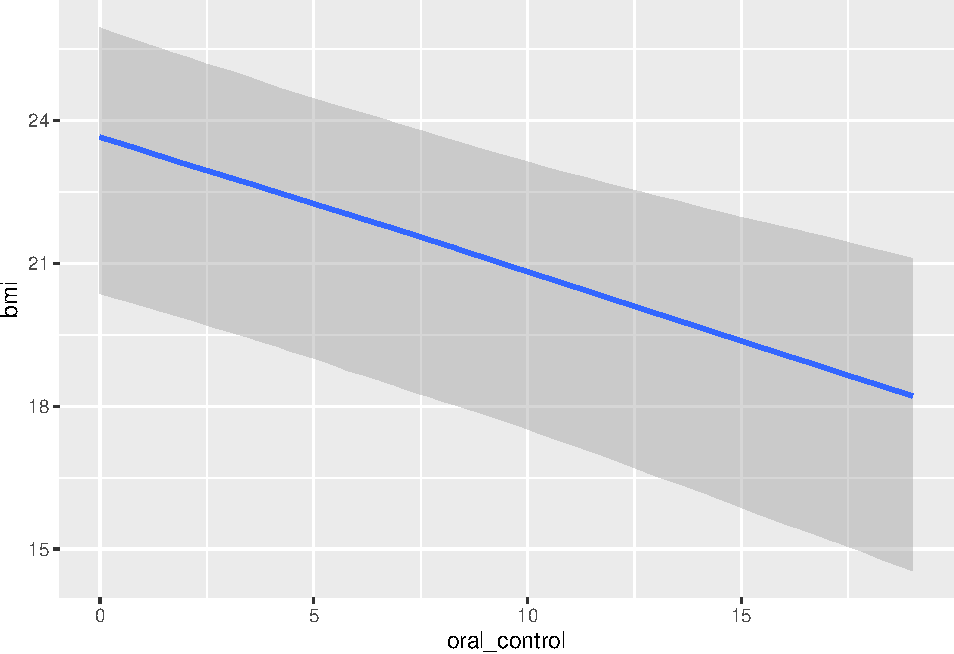
\includegraphics{050_quest_groups_files/figure-latex/unnamed-chunk-1-2.pdf}

\begin{Shaded}
\begin{Highlighting}[]
\FunctionTok{plot}\NormalTok{(}\FunctionTok{conditional\_effects}\NormalTok{(m1, }\StringTok{"dieting"}\NormalTok{))}
\end{Highlighting}
\end{Shaded}

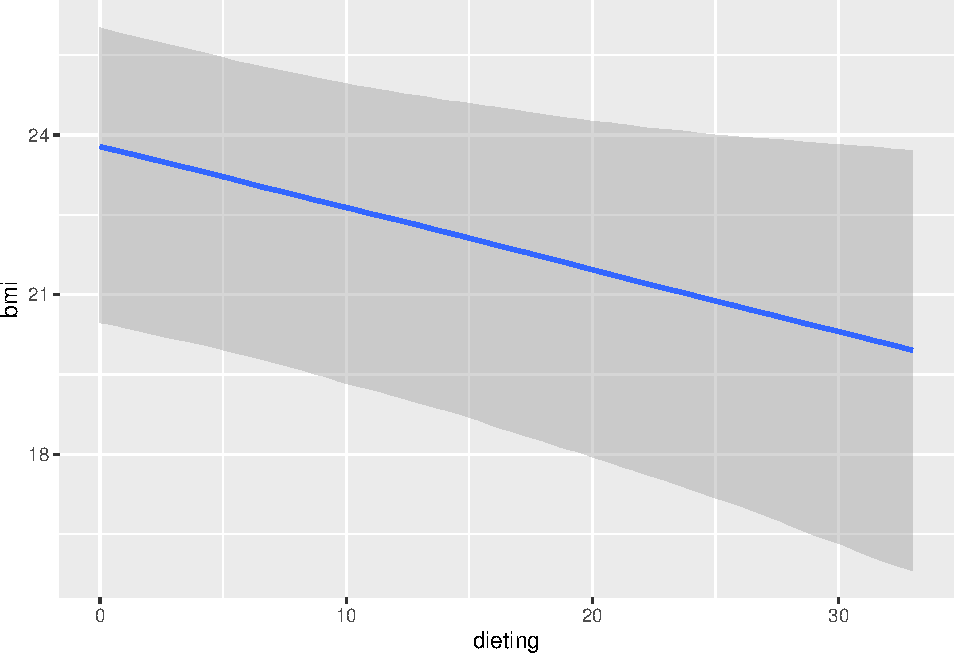
\includegraphics{050_quest_groups_files/figure-latex/unnamed-chunk-1-3.pdf}

\begin{Shaded}
\begin{Highlighting}[]
\FunctionTok{plot}\NormalTok{(}\FunctionTok{conditional\_effects}\NormalTok{(m1, }\StringTok{"bsq14\_tot"}\NormalTok{))}
\end{Highlighting}
\end{Shaded}

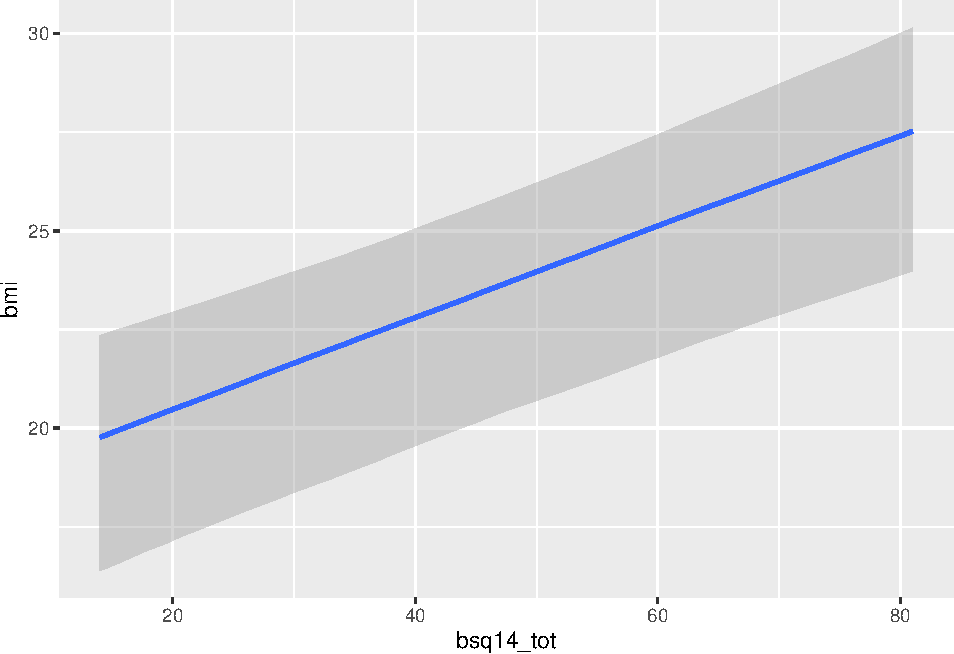
\includegraphics{050_quest_groups_files/figure-latex/unnamed-chunk-1-4.pdf}

\begin{Shaded}
\begin{Highlighting}[]
\FunctionTok{plot}\NormalTok{(}\FunctionTok{conditional\_effects}\NormalTok{(m1, }\StringTok{"ros\_tot"}\NormalTok{))}
\end{Highlighting}
\end{Shaded}

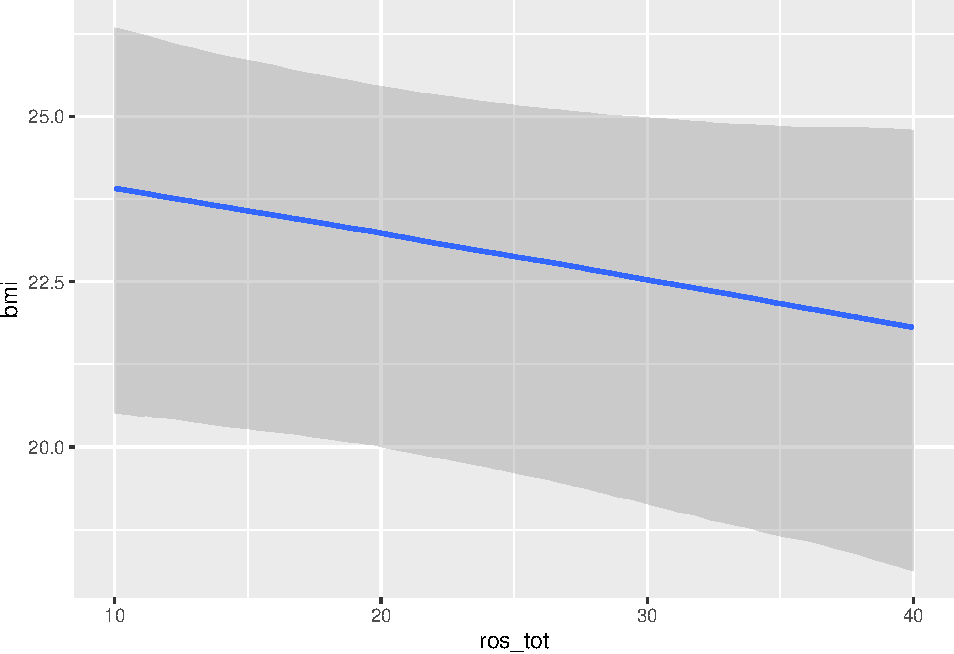
\includegraphics{050_quest_groups_files/figure-latex/unnamed-chunk-1-5.pdf}

\begin{Shaded}
\begin{Highlighting}[]
\FunctionTok{plot}\NormalTok{(}\FunctionTok{conditional\_effects}\NormalTok{(m1, }\StringTok{"mps\_cmd"}\NormalTok{))}
\end{Highlighting}
\end{Shaded}

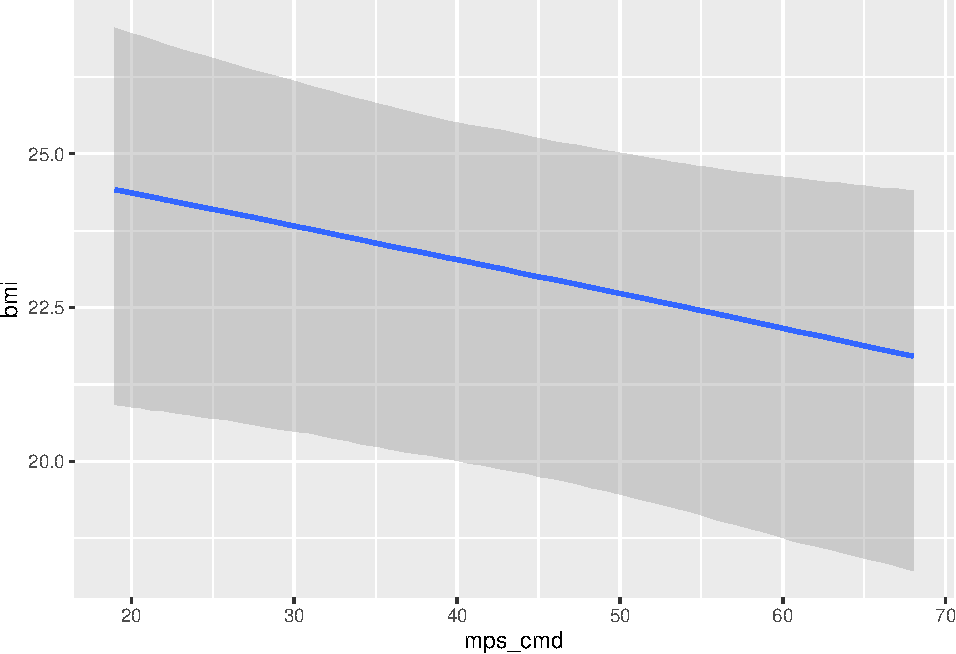
\includegraphics{050_quest_groups_files/figure-latex/unnamed-chunk-1-6.pdf}

\begin{Shaded}
\begin{Highlighting}[]
\FunctionTok{plot}\NormalTok{(}\FunctionTok{conditional\_effects}\NormalTok{(m1, }\StringTok{"age"}\NormalTok{))}
\end{Highlighting}
\end{Shaded}

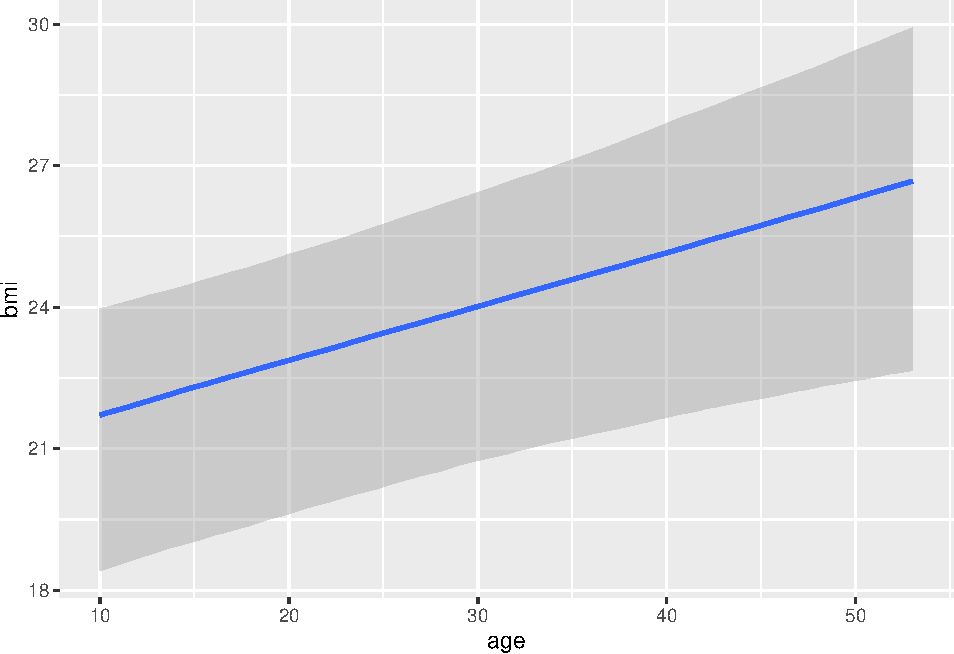
\includegraphics{050_quest_groups_files/figure-latex/unnamed-chunk-1-7.pdf}

\begin{Shaded}
\begin{Highlighting}[]
\FunctionTok{bayes\_R2}\NormalTok{(m1)}
\end{Highlighting}
\end{Shaded}

\begin{verbatim}
##     Estimate  Est.Error      Q2.5     Q97.5
## R2 0.3084927 0.03378923 0.2399049 0.3729437
\end{verbatim}

\begin{Shaded}
\begin{Highlighting}[]
\FunctionTok{hist}\NormalTok{(quest\_data2}\SpecialCharTok{$}\NormalTok{age)}
\end{Highlighting}
\end{Shaded}

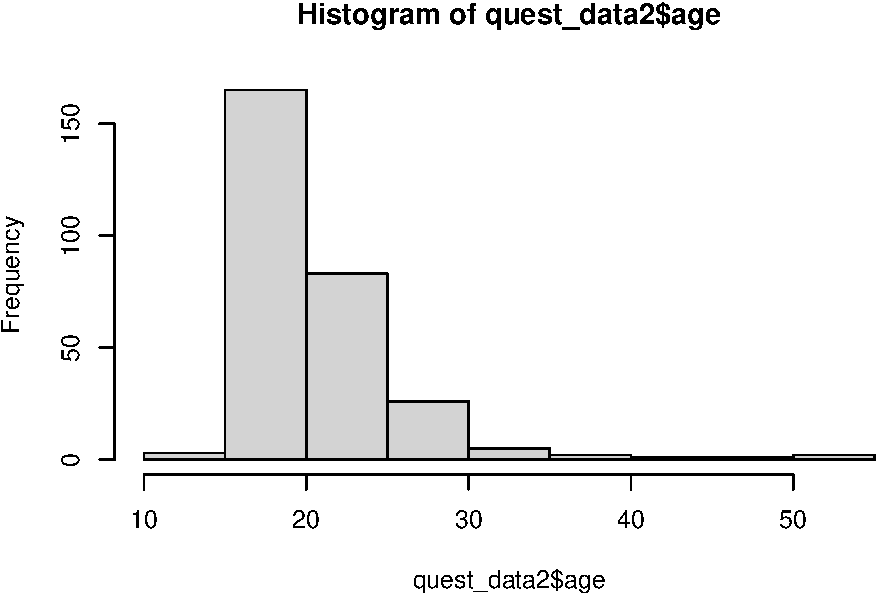
\includegraphics{050_quest_groups_files/figure-latex/unnamed-chunk-1-8.pdf}

Gender-Dependent Associations of Anxiety and Depression Symptoms With
Eating Disorder Psychopathology in a Representative Population Sample
Mareike Ernst, Antonia M. Werner, Ana N. Tibubos, Manfred E. Beutel,
MartinadeZwaan and ElmarBrähler

\begin{Shaded}
\begin{Highlighting}[]
\FunctionTok{table}\NormalTok{(quest\_data2}\SpecialCharTok{$}\NormalTok{sex)}
\end{Highlighting}
\end{Shaded}

\begin{verbatim}
## 
##   Altro Femmina Maschio 
##       4     244      40
\end{verbatim}

\begin{Shaded}
\begin{Highlighting}[]
\FunctionTok{hist}\NormalTok{(quest\_data2}\SpecialCharTok{$}\NormalTok{eat26\_tot)}
\end{Highlighting}
\end{Shaded}

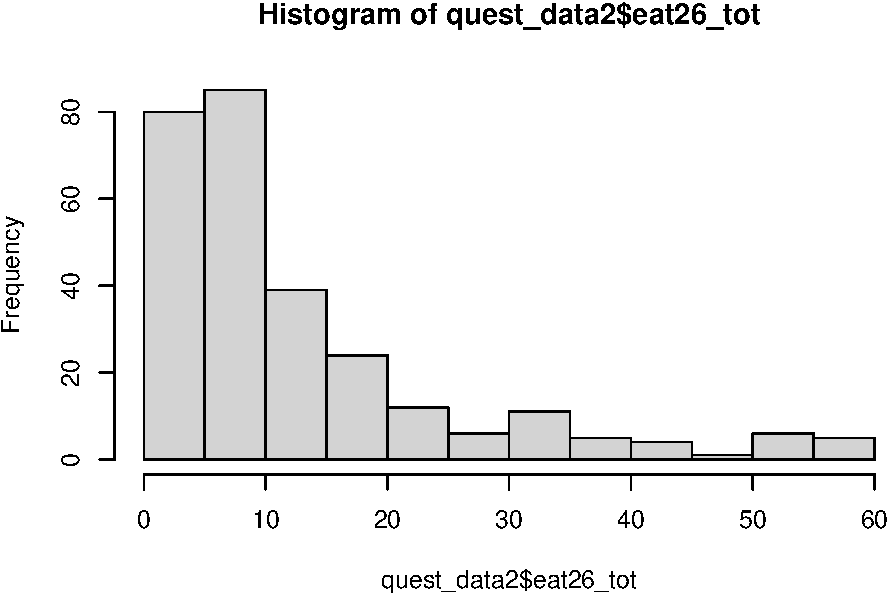
\includegraphics{050_quest_groups_files/figure-latex/unnamed-chunk-2-1.pdf}

\begin{Shaded}
\begin{Highlighting}[]
\NormalTok{quest\_data2}\SpecialCharTok{$}\NormalTok{is\_patient }\OtherTok{\textless{}{-}} \FunctionTok{factor}\NormalTok{(quest\_data2}\SpecialCharTok{$}\NormalTok{is\_patient)}

\NormalTok{quest\_data3 }\OtherTok{\textless{}{-}}\NormalTok{ quest\_data2 }\SpecialCharTok{\%\textgreater{}\%} 
\NormalTok{  dplyr}\SpecialCharTok{::}\FunctionTok{filter}\NormalTok{(sex }\SpecialCharTok{!=} \StringTok{"Altro"}\NormalTok{)}

\NormalTok{m3 }\OtherTok{\textless{}{-}} \FunctionTok{brm}\NormalTok{(}
\NormalTok{  eat26\_tot }\SpecialCharTok{\textasciitilde{}}\NormalTok{ bmi }\SpecialCharTok{+}\NormalTok{ age }\SpecialCharTok{+}\NormalTok{ (dass21\_anxiety }\SpecialCharTok{+}\NormalTok{ dass21\_dep) }\SpecialCharTok{*}\NormalTok{ (is\_patient }\SpecialCharTok{+}\NormalTok{ sex),}
  \AttributeTok{data =}\NormalTok{ quest\_data3, }
  \CommentTok{\# prior = prior\_ma,}
  \AttributeTok{family =} \FunctionTok{skew\_normal}\NormalTok{(),}
  \AttributeTok{control =} \FunctionTok{list}\NormalTok{(}\AttributeTok{adapt\_delta =} \FloatTok{0.98}\NormalTok{),}
  \AttributeTok{iter =} \DecValTok{4000}\NormalTok{,}
  \AttributeTok{cores =} \DecValTok{6}\NormalTok{,}
  \AttributeTok{backend =} \StringTok{"cmdstan"}
\NormalTok{)}
\end{Highlighting}
\end{Shaded}

\begin{verbatim}
## Warning: Rows containing NAs were excluded from the model.
\end{verbatim}

\begin{verbatim}
## Start sampling
\end{verbatim}

\begin{verbatim}
## Running MCMC with 4 chains, at most 6 in parallel...
## 
## Chain 1 Iteration:    1 / 4000 [  0%]  (Warmup) 
## Chain 2 Iteration:    1 / 4000 [  0%]  (Warmup)
\end{verbatim}

\begin{verbatim}
## Chain 3 Rejecting initial value:
\end{verbatim}

\begin{verbatim}
## Chain 3   Log probability evaluates to log(0), i.e. negative infinity.
\end{verbatim}

\begin{verbatim}
## Chain 3   Stan can't start sampling from this initial value.
\end{verbatim}

\begin{verbatim}
## Chain 3 Rejecting initial value:
\end{verbatim}

\begin{verbatim}
## Chain 3   Log probability evaluates to log(0), i.e. negative infinity.
\end{verbatim}

\begin{verbatim}
## Chain 3   Stan can't start sampling from this initial value.
\end{verbatim}

\begin{verbatim}
## Chain 3 Iteration:    1 / 4000 [  0%]  (Warmup) 
## Chain 4 Iteration:    1 / 4000 [  0%]  (Warmup) 
## Chain 1 Iteration:  100 / 4000 [  2%]  (Warmup) 
## Chain 2 Iteration:  100 / 4000 [  2%]  (Warmup) 
## Chain 4 Iteration:  100 / 4000 [  2%]  (Warmup) 
## Chain 1 Iteration:  200 / 4000 [  5%]  (Warmup) 
## Chain 3 Iteration:  100 / 4000 [  2%]  (Warmup) 
## Chain 1 Iteration:  300 / 4000 [  7%]  (Warmup) 
## Chain 2 Iteration:  200 / 4000 [  5%]  (Warmup) 
## Chain 3 Iteration:  200 / 4000 [  5%]  (Warmup) 
## Chain 4 Iteration:  200 / 4000 [  5%]  (Warmup) 
## Chain 1 Iteration:  400 / 4000 [ 10%]  (Warmup) 
## Chain 3 Iteration:  300 / 4000 [  7%]  (Warmup) 
## Chain 4 Iteration:  300 / 4000 [  7%]  (Warmup) 
## Chain 1 Iteration:  500 / 4000 [ 12%]  (Warmup) 
## Chain 2 Iteration:  300 / 4000 [  7%]  (Warmup) 
## Chain 3 Iteration:  400 / 4000 [ 10%]  (Warmup) 
## Chain 1 Iteration:  600 / 4000 [ 15%]  (Warmup) 
## Chain 2 Iteration:  400 / 4000 [ 10%]  (Warmup) 
## Chain 4 Iteration:  400 / 4000 [ 10%]  (Warmup) 
## Chain 1 Iteration:  700 / 4000 [ 17%]  (Warmup) 
## Chain 2 Iteration:  500 / 4000 [ 12%]  (Warmup) 
## Chain 3 Iteration:  500 / 4000 [ 12%]  (Warmup) 
## Chain 4 Iteration:  500 / 4000 [ 12%]  (Warmup) 
## Chain 1 Iteration:  800 / 4000 [ 20%]  (Warmup) 
## Chain 2 Iteration:  600 / 4000 [ 15%]  (Warmup) 
## Chain 3 Iteration:  600 / 4000 [ 15%]  (Warmup) 
## Chain 4 Iteration:  600 / 4000 [ 15%]  (Warmup) 
## Chain 1 Iteration:  900 / 4000 [ 22%]  (Warmup) 
## Chain 2 Iteration:  700 / 4000 [ 17%]  (Warmup) 
## Chain 3 Iteration:  700 / 4000 [ 17%]  (Warmup) 
## Chain 1 Iteration: 1000 / 4000 [ 25%]  (Warmup) 
## Chain 2 Iteration:  800 / 4000 [ 20%]  (Warmup) 
## Chain 3 Iteration:  800 / 4000 [ 20%]  (Warmup) 
## Chain 4 Iteration:  700 / 4000 [ 17%]  (Warmup) 
## Chain 1 Iteration: 1100 / 4000 [ 27%]  (Warmup) 
## Chain 4 Iteration:  800 / 4000 [ 20%]  (Warmup) 
## Chain 3 Iteration:  900 / 4000 [ 22%]  (Warmup) 
## Chain 1 Iteration: 1200 / 4000 [ 30%]  (Warmup) 
## Chain 2 Iteration:  900 / 4000 [ 22%]  (Warmup) 
## Chain 4 Iteration:  900 / 4000 [ 22%]  (Warmup) 
## Chain 1 Iteration: 1300 / 4000 [ 32%]  (Warmup) 
## Chain 2 Iteration: 1000 / 4000 [ 25%]  (Warmup) 
## Chain 3 Iteration: 1000 / 4000 [ 25%]  (Warmup) 
## Chain 4 Iteration: 1000 / 4000 [ 25%]  (Warmup) 
## Chain 1 Iteration: 1400 / 4000 [ 35%]  (Warmup) 
## Chain 2 Iteration: 1100 / 4000 [ 27%]  (Warmup) 
## Chain 3 Iteration: 1100 / 4000 [ 27%]  (Warmup) 
## Chain 4 Iteration: 1100 / 4000 [ 27%]  (Warmup) 
## Chain 3 Iteration: 1200 / 4000 [ 30%]  (Warmup) 
## Chain 4 Iteration: 1200 / 4000 [ 30%]  (Warmup) 
## Chain 1 Iteration: 1500 / 4000 [ 37%]  (Warmup) 
## Chain 2 Iteration: 1200 / 4000 [ 30%]  (Warmup) 
## Chain 3 Iteration: 1300 / 4000 [ 32%]  (Warmup) 
## Chain 1 Iteration: 1600 / 4000 [ 40%]  (Warmup) 
## Chain 2 Iteration: 1300 / 4000 [ 32%]  (Warmup) 
## Chain 4 Iteration: 1300 / 4000 [ 32%]  (Warmup) 
## Chain 1 Iteration: 1700 / 4000 [ 42%]  (Warmup) 
## Chain 2 Iteration: 1400 / 4000 [ 35%]  (Warmup) 
## Chain 3 Iteration: 1400 / 4000 [ 35%]  (Warmup) 
## Chain 4 Iteration: 1400 / 4000 [ 35%]  (Warmup) 
## Chain 1 Iteration: 1800 / 4000 [ 45%]  (Warmup) 
## Chain 3 Iteration: 1500 / 4000 [ 37%]  (Warmup) 
## Chain 4 Iteration: 1500 / 4000 [ 37%]  (Warmup) 
## Chain 2 Iteration: 1500 / 4000 [ 37%]  (Warmup) 
## Chain 3 Iteration: 1600 / 4000 [ 40%]  (Warmup) 
## Chain 1 Iteration: 1900 / 4000 [ 47%]  (Warmup) 
## Chain 2 Iteration: 1600 / 4000 [ 40%]  (Warmup) 
## Chain 4 Iteration: 1600 / 4000 [ 40%]  (Warmup) 
## Chain 1 Iteration: 2000 / 4000 [ 50%]  (Warmup) 
## Chain 1 Iteration: 2001 / 4000 [ 50%]  (Sampling) 
## Chain 2 Iteration: 1700 / 4000 [ 42%]  (Warmup) 
## Chain 3 Iteration: 1700 / 4000 [ 42%]  (Warmup) 
## Chain 4 Iteration: 1700 / 4000 [ 42%]  (Warmup) 
## Chain 3 Iteration: 1800 / 4000 [ 45%]  (Warmup) 
## Chain 4 Iteration: 1800 / 4000 [ 45%]  (Warmup) 
## Chain 1 Iteration: 2100 / 4000 [ 52%]  (Sampling) 
## Chain 2 Iteration: 1800 / 4000 [ 45%]  (Warmup) 
## Chain 3 Iteration: 1900 / 4000 [ 47%]  (Warmup) 
## Chain 4 Iteration: 1900 / 4000 [ 47%]  (Warmup) 
## Chain 1 Iteration: 2200 / 4000 [ 55%]  (Sampling) 
## Chain 2 Iteration: 1900 / 4000 [ 47%]  (Warmup) 
## Chain 1 Iteration: 2300 / 4000 [ 57%]  (Sampling) 
## Chain 2 Iteration: 2000 / 4000 [ 50%]  (Warmup) 
## Chain 2 Iteration: 2001 / 4000 [ 50%]  (Sampling) 
## Chain 3 Iteration: 2000 / 4000 [ 50%]  (Warmup) 
## Chain 3 Iteration: 2001 / 4000 [ 50%]  (Sampling) 
## Chain 1 Iteration: 2400 / 4000 [ 60%]  (Sampling) 
## Chain 3 Iteration: 2100 / 4000 [ 52%]  (Sampling) 
## Chain 4 Iteration: 2000 / 4000 [ 50%]  (Warmup) 
## Chain 4 Iteration: 2001 / 4000 [ 50%]  (Sampling) 
## Chain 1 Iteration: 2500 / 4000 [ 62%]  (Sampling) 
## Chain 2 Iteration: 2100 / 4000 [ 52%]  (Sampling) 
## Chain 4 Iteration: 2100 / 4000 [ 52%]  (Sampling) 
## Chain 2 Iteration: 2200 / 4000 [ 55%]  (Sampling) 
## Chain 3 Iteration: 2200 / 4000 [ 55%]  (Sampling) 
## Chain 1 Iteration: 2600 / 4000 [ 65%]  (Sampling) 
## Chain 2 Iteration: 2300 / 4000 [ 57%]  (Sampling) 
## Chain 3 Iteration: 2300 / 4000 [ 57%]  (Sampling) 
## Chain 4 Iteration: 2200 / 4000 [ 55%]  (Sampling) 
## Chain 1 Iteration: 2700 / 4000 [ 67%]  (Sampling) 
## Chain 2 Iteration: 2400 / 4000 [ 60%]  (Sampling) 
## Chain 3 Iteration: 2400 / 4000 [ 60%]  (Sampling) 
## Chain 4 Iteration: 2300 / 4000 [ 57%]  (Sampling) 
## Chain 1 Iteration: 2800 / 4000 [ 70%]  (Sampling) 
## Chain 3 Iteration: 2500 / 4000 [ 62%]  (Sampling) 
## Chain 1 Iteration: 2900 / 4000 [ 72%]  (Sampling) 
## Chain 2 Iteration: 2500 / 4000 [ 62%]  (Sampling) 
## Chain 4 Iteration: 2400 / 4000 [ 60%]  (Sampling) 
## Chain 1 Iteration: 3000 / 4000 [ 75%]  (Sampling) 
## Chain 2 Iteration: 2600 / 4000 [ 65%]  (Sampling) 
## Chain 3 Iteration: 2600 / 4000 [ 65%]  (Sampling) 
## Chain 4 Iteration: 2500 / 4000 [ 62%]  (Sampling) 
## Chain 1 Iteration: 3100 / 4000 [ 77%]  (Sampling) 
## Chain 2 Iteration: 2700 / 4000 [ 67%]  (Sampling) 
## Chain 3 Iteration: 2700 / 4000 [ 67%]  (Sampling) 
## Chain 2 Iteration: 2800 / 4000 [ 70%]  (Sampling) 
## Chain 3 Iteration: 2800 / 4000 [ 70%]  (Sampling) 
## Chain 4 Iteration: 2600 / 4000 [ 65%]  (Sampling) 
## Chain 1 Iteration: 3200 / 4000 [ 80%]  (Sampling) 
## Chain 3 Iteration: 2900 / 4000 [ 72%]  (Sampling) 
## Chain 4 Iteration: 2700 / 4000 [ 67%]  (Sampling) 
## Chain 1 Iteration: 3300 / 4000 [ 82%]  (Sampling) 
## Chain 2 Iteration: 2900 / 4000 [ 72%]  (Sampling) 
## Chain 4 Iteration: 2800 / 4000 [ 70%]  (Sampling) 
## Chain 1 Iteration: 3400 / 4000 [ 85%]  (Sampling) 
## Chain 2 Iteration: 3000 / 4000 [ 75%]  (Sampling) 
## Chain 3 Iteration: 3000 / 4000 [ 75%]  (Sampling) 
## Chain 1 Iteration: 3500 / 4000 [ 87%]  (Sampling) 
## Chain 2 Iteration: 3100 / 4000 [ 77%]  (Sampling) 
## Chain 3 Iteration: 3100 / 4000 [ 77%]  (Sampling) 
## Chain 4 Iteration: 2900 / 4000 [ 72%]  (Sampling) 
## Chain 2 Iteration: 3200 / 4000 [ 80%]  (Sampling) 
## Chain 3 Iteration: 3200 / 4000 [ 80%]  (Sampling) 
## Chain 4 Iteration: 3000 / 4000 [ 75%]  (Sampling) 
## Chain 1 Iteration: 3600 / 4000 [ 90%]  (Sampling) 
## Chain 3 Iteration: 3300 / 4000 [ 82%]  (Sampling) 
## Chain 1 Iteration: 3700 / 4000 [ 92%]  (Sampling) 
## Chain 2 Iteration: 3300 / 4000 [ 82%]  (Sampling) 
## Chain 4 Iteration: 3100 / 4000 [ 77%]  (Sampling) 
## Chain 1 Iteration: 3800 / 4000 [ 95%]  (Sampling) 
## Chain 2 Iteration: 3400 / 4000 [ 85%]  (Sampling) 
## Chain 3 Iteration: 3400 / 4000 [ 85%]  (Sampling) 
## Chain 4 Iteration: 3200 / 4000 [ 80%]  (Sampling) 
## Chain 1 Iteration: 3900 / 4000 [ 97%]  (Sampling) 
## Chain 2 Iteration: 3500 / 4000 [ 87%]  (Sampling) 
## Chain 3 Iteration: 3500 / 4000 [ 87%]  (Sampling) 
## Chain 2 Iteration: 3600 / 4000 [ 90%]  (Sampling) 
## Chain 3 Iteration: 3600 / 4000 [ 90%]  (Sampling) 
## Chain 4 Iteration: 3300 / 4000 [ 82%]  (Sampling) 
## Chain 1 Iteration: 4000 / 4000 [100%]  (Sampling) 
## Chain 3 Iteration: 3700 / 4000 [ 92%]  (Sampling) 
## Chain 4 Iteration: 3400 / 4000 [ 85%]  (Sampling) 
## Chain 1 finished in 6.1 seconds.
## Chain 2 Iteration: 3700 / 4000 [ 92%]  (Sampling) 
## Chain 3 Iteration: 3800 / 4000 [ 95%]  (Sampling) 
## Chain 2 Iteration: 3800 / 4000 [ 95%]  (Sampling) 
## Chain 4 Iteration: 3500 / 4000 [ 87%]  (Sampling) 
## Chain 2 Iteration: 3900 / 4000 [ 97%]  (Sampling) 
## Chain 3 Iteration: 3900 / 4000 [ 97%]  (Sampling) 
## Chain 4 Iteration: 3600 / 4000 [ 90%]  (Sampling) 
## Chain 2 Iteration: 4000 / 4000 [100%]  (Sampling) 
## Chain 3 Iteration: 4000 / 4000 [100%]  (Sampling) 
## Chain 2 finished in 6.6 seconds.
## Chain 3 finished in 6.5 seconds.
## Chain 4 Iteration: 3700 / 4000 [ 92%]  (Sampling) 
## Chain 4 Iteration: 3800 / 4000 [ 95%]  (Sampling) 
## Chain 4 Iteration: 3900 / 4000 [ 97%]  (Sampling) 
## Chain 4 Iteration: 4000 / 4000 [100%]  (Sampling) 
## Chain 4 finished in 7.0 seconds.
## 
## All 4 chains finished successfully.
## Mean chain execution time: 6.6 seconds.
## Total execution time: 7.3 seconds.
\end{verbatim}

\begin{Shaded}
\begin{Highlighting}[]
\FunctionTok{summary}\NormalTok{(m3)}
\end{Highlighting}
\end{Shaded}

\begin{verbatim}
##  Family: skew_normal 
##   Links: mu = identity; sigma = identity; alpha = identity 
## Formula: eat26_tot ~ bmi + age + (dass21_anxiety + dass21_dep) * (is_patient + sex) 
##    Data: quest_data3 (Number of observations: 265) 
## Samples: 4 chains, each with iter = 4000; warmup = 2000; thin = 1;
##          total post-warmup samples = 8000
## 
## Population-Level Effects: 
##                            Estimate Est.Error l-95% CI u-95% CI Rhat Bulk_ESS
## Intercept                     19.62      2.72    14.29    24.94 1.00     7666
## bmi                           -0.13      0.12    -0.38     0.10 1.00     7057
## age                           -0.19      0.09    -0.36    -0.03 1.00     6078
## dass21_anxiety                -0.01      0.11    -0.22     0.19 1.00     5815
## dass21_dep                     0.18      0.10     0.00     0.37 1.00     5067
## is_patient1                   14.30      5.44     2.44    23.16 1.00     4734
## sexMaschio                    -0.42      2.19    -5.23     3.39 1.00     5529
## dass21_anxiety:is_patient1     1.26      0.50     0.24     2.16 1.00     5732
## dass21_anxiety:sexMaschio      0.03      0.30    -0.60     0.63 1.00     6633
## dass21_dep:is_patient1        -1.32      0.40    -2.09    -0.52 1.00     5136
## dass21_dep:sexMaschio         -0.17      0.23    -0.65     0.25 1.00     5697
##                            Tail_ESS
## Intercept                      6406
## bmi                            5337
## age                            5773
## dass21_anxiety                 5658
## dass21_dep                     5798
## is_patient1                    4342
## sexMaschio                     4416
## dass21_anxiety:is_patient1     5190
## dass21_anxiety:sexMaschio      5223
## dass21_dep:is_patient1         5783
## dass21_dep:sexMaschio          4543
## 
## Family Specific Parameters: 
##       Estimate Est.Error l-95% CI u-95% CI Rhat Bulk_ESS Tail_ESS
## sigma     9.06      0.42     8.29     9.92 1.00     5964     5186
## alpha     9.96      2.12     6.43    14.58 1.00     6068     5070
## 
## Samples were drawn using sample(hmc). For each parameter, Bulk_ESS
## and Tail_ESS are effective sample size measures, and Rhat is the potential
## scale reduction factor on split chains (at convergence, Rhat = 1).
\end{verbatim}

\begin{Shaded}
\begin{Highlighting}[]
\FunctionTok{plot}\NormalTok{(}\FunctionTok{conditional\_effects}\NormalTok{(m3, }\StringTok{"dass21\_anxiety:is\_patient"}\NormalTok{))}
\end{Highlighting}
\end{Shaded}

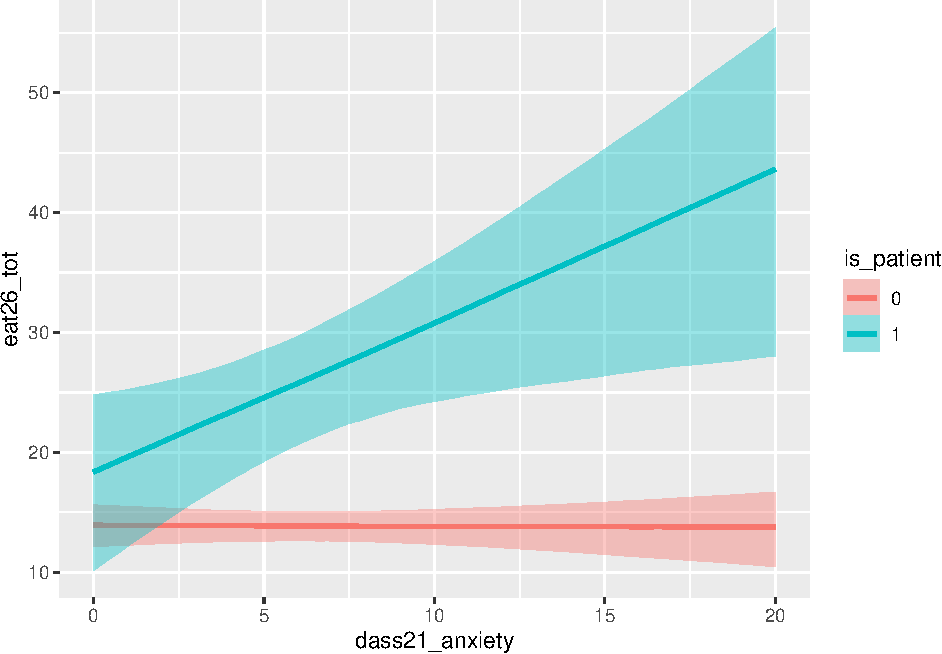
\includegraphics{050_quest_groups_files/figure-latex/unnamed-chunk-2-2.pdf}

\begin{Shaded}
\begin{Highlighting}[]
\FunctionTok{plot}\NormalTok{(}\FunctionTok{conditional\_effects}\NormalTok{(m3, }\StringTok{"dass21\_dep:is\_patient"}\NormalTok{))}
\end{Highlighting}
\end{Shaded}

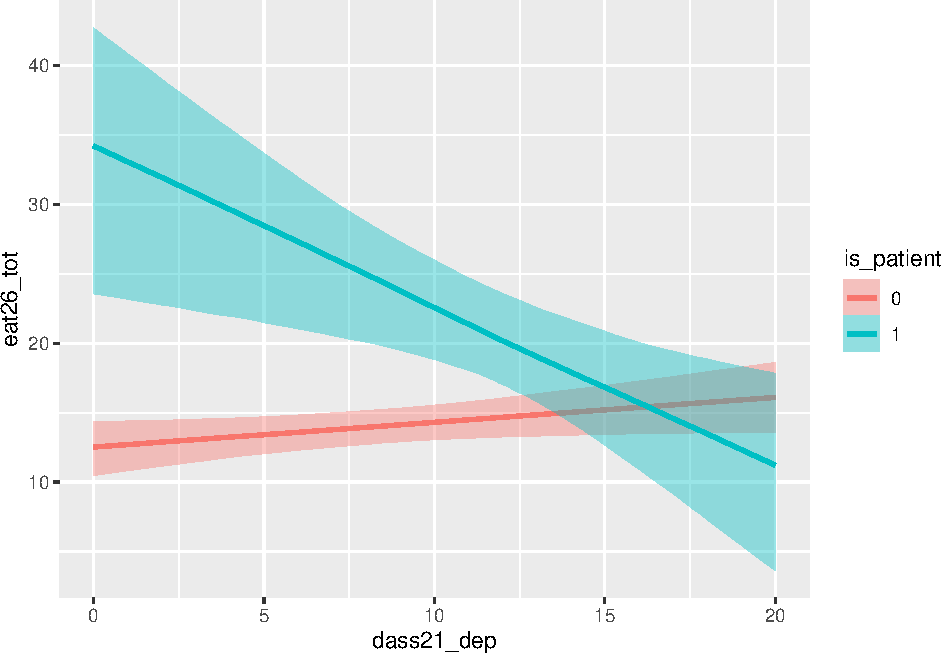
\includegraphics{050_quest_groups_files/figure-latex/unnamed-chunk-2-3.pdf}

\begin{Shaded}
\begin{Highlighting}[]
\FunctionTok{plot}\NormalTok{(}\FunctionTok{conditional\_effects}\NormalTok{(m3, }\StringTok{"dass21\_dep"}\NormalTok{))}
\end{Highlighting}
\end{Shaded}

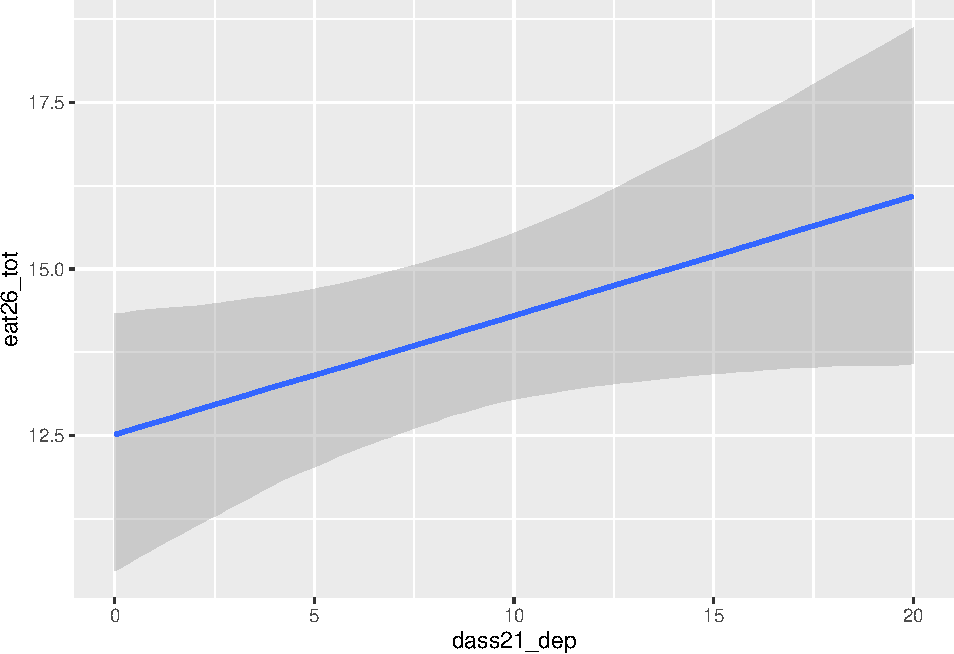
\includegraphics{050_quest_groups_files/figure-latex/unnamed-chunk-2-4.pdf}

\begin{Shaded}
\begin{Highlighting}[]
\FunctionTok{plot}\NormalTok{(}\FunctionTok{conditional\_effects}\NormalTok{(m3, }\StringTok{"is\_patient"}\NormalTok{))}
\end{Highlighting}
\end{Shaded}

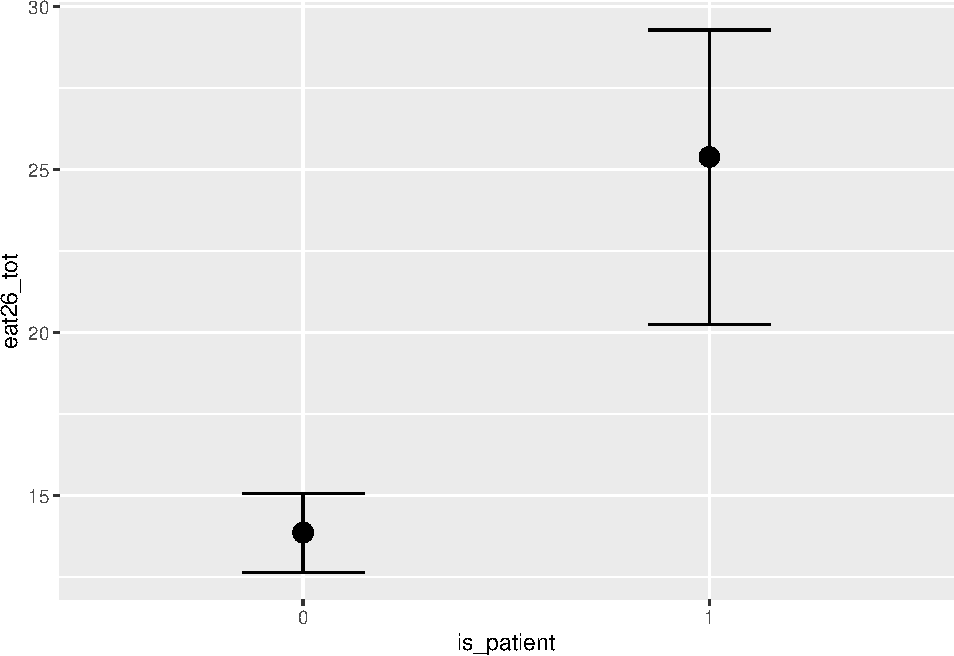
\includegraphics{050_quest_groups_files/figure-latex/unnamed-chunk-2-5.pdf}

\begin{Shaded}
\begin{Highlighting}[]
\FunctionTok{plot}\NormalTok{(}\FunctionTok{conditional\_effects}\NormalTok{(m3, }\StringTok{"age"}\NormalTok{))}
\end{Highlighting}
\end{Shaded}

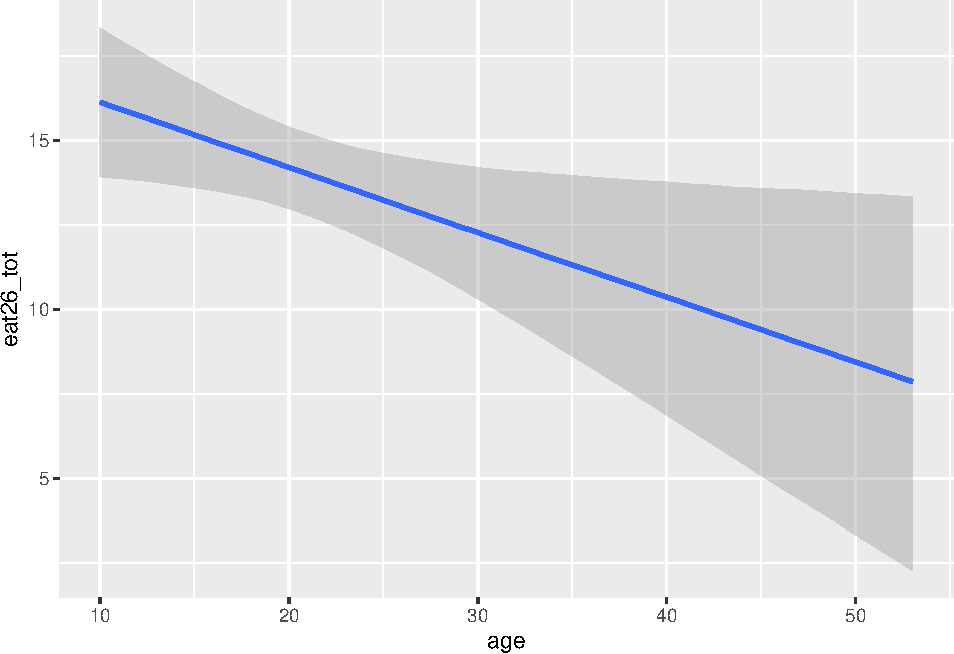
\includegraphics{050_quest_groups_files/figure-latex/unnamed-chunk-2-6.pdf}

\begin{Shaded}
\begin{Highlighting}[]
\NormalTok{m4 }\OtherTok{\textless{}{-}} \FunctionTok{brm}\NormalTok{(}
\NormalTok{  eat26\_tot }\SpecialCharTok{\textasciitilde{}}\NormalTok{ bmi }\SpecialCharTok{+}\NormalTok{ age }\SpecialCharTok{+}\NormalTok{ (dass21\_anxiety }\SpecialCharTok{+}\NormalTok{ dass21\_dep),}
  \AttributeTok{data =}\NormalTok{ quest\_data3[quest\_data3}\SpecialCharTok{$}\NormalTok{sex }\SpecialCharTok{==} \StringTok{"Femmina"}\NormalTok{, ], }
  \CommentTok{\# prior = prior\_ma,}
  \AttributeTok{family =} \FunctionTok{skew\_normal}\NormalTok{(),}
  \AttributeTok{control =} \FunctionTok{list}\NormalTok{(}\AttributeTok{adapt\_delta =} \FloatTok{0.98}\NormalTok{),}
  \AttributeTok{iter =} \DecValTok{4000}\NormalTok{,}
  \AttributeTok{cores =} \DecValTok{6}\NormalTok{,}
  \AttributeTok{backend =} \StringTok{"cmdstan"}
\NormalTok{)}
\end{Highlighting}
\end{Shaded}

\begin{verbatim}
## Warning: Rows containing NAs were excluded from the model.
\end{verbatim}

\begin{verbatim}
## Start sampling
\end{verbatim}

\begin{verbatim}
## Running MCMC with 4 chains, at most 6 in parallel...
## 
## Chain 1 Iteration:    1 / 4000 [  0%]  (Warmup) 
## Chain 2 Iteration:    1 / 4000 [  0%]  (Warmup)
\end{verbatim}

\begin{verbatim}
## Chain 3 Rejecting initial value:
\end{verbatim}

\begin{verbatim}
## Chain 3   Log probability evaluates to log(0), i.e. negative infinity.
\end{verbatim}

\begin{verbatim}
## Chain 3   Stan can't start sampling from this initial value.
\end{verbatim}

\begin{verbatim}
## Chain 3 Iteration:    1 / 4000 [  0%]  (Warmup) 
## Chain 4 Iteration:    1 / 4000 [  0%]  (Warmup) 
## Chain 1 Iteration:  100 / 4000 [  2%]  (Warmup) 
## Chain 4 Iteration:  100 / 4000 [  2%]  (Warmup) 
## Chain 1 Iteration:  200 / 4000 [  5%]  (Warmup) 
## Chain 1 Iteration:  300 / 4000 [  7%]  (Warmup) 
## Chain 2 Iteration:  100 / 4000 [  2%]  (Warmup) 
## Chain 2 Iteration:  200 / 4000 [  5%]  (Warmup) 
## Chain 3 Iteration:  100 / 4000 [  2%]  (Warmup) 
## Chain 3 Iteration:  200 / 4000 [  5%]  (Warmup) 
## Chain 4 Iteration:  200 / 4000 [  5%]  (Warmup) 
## Chain 4 Iteration:  300 / 4000 [  7%]  (Warmup) 
## Chain 4 Iteration:  400 / 4000 [ 10%]  (Warmup) 
## Chain 1 Iteration:  400 / 4000 [ 10%]  (Warmup) 
## Chain 1 Iteration:  500 / 4000 [ 12%]  (Warmup) 
## Chain 1 Iteration:  600 / 4000 [ 15%]  (Warmup) 
## Chain 2 Iteration:  300 / 4000 [  7%]  (Warmup) 
## Chain 2 Iteration:  400 / 4000 [ 10%]  (Warmup) 
## Chain 3 Iteration:  300 / 4000 [  7%]  (Warmup) 
## Chain 3 Iteration:  400 / 4000 [ 10%]  (Warmup) 
## Chain 3 Iteration:  500 / 4000 [ 12%]  (Warmup) 
## Chain 4 Iteration:  500 / 4000 [ 12%]  (Warmup) 
## Chain 4 Iteration:  600 / 4000 [ 15%]  (Warmup) 
## Chain 1 Iteration:  700 / 4000 [ 17%]  (Warmup) 
## Chain 1 Iteration:  800 / 4000 [ 20%]  (Warmup) 
## Chain 1 Iteration:  900 / 4000 [ 22%]  (Warmup) 
## Chain 2 Iteration:  500 / 4000 [ 12%]  (Warmup) 
## Chain 2 Iteration:  600 / 4000 [ 15%]  (Warmup) 
## Chain 2 Iteration:  700 / 4000 [ 17%]  (Warmup) 
## Chain 3 Iteration:  600 / 4000 [ 15%]  (Warmup) 
## Chain 3 Iteration:  700 / 4000 [ 17%]  (Warmup) 
## Chain 3 Iteration:  800 / 4000 [ 20%]  (Warmup) 
## Chain 4 Iteration:  700 / 4000 [ 17%]  (Warmup) 
## Chain 4 Iteration:  800 / 4000 [ 20%]  (Warmup) 
## Chain 1 Iteration: 1000 / 4000 [ 25%]  (Warmup) 
## Chain 1 Iteration: 1100 / 4000 [ 27%]  (Warmup) 
## Chain 1 Iteration: 1200 / 4000 [ 30%]  (Warmup) 
## Chain 2 Iteration:  800 / 4000 [ 20%]  (Warmup) 
## Chain 2 Iteration:  900 / 4000 [ 22%]  (Warmup) 
## Chain 2 Iteration: 1000 / 4000 [ 25%]  (Warmup) 
## Chain 3 Iteration:  900 / 4000 [ 22%]  (Warmup) 
## Chain 3 Iteration: 1000 / 4000 [ 25%]  (Warmup) 
## Chain 3 Iteration: 1100 / 4000 [ 27%]  (Warmup) 
## Chain 4 Iteration:  900 / 4000 [ 22%]  (Warmup) 
## Chain 4 Iteration: 1000 / 4000 [ 25%]  (Warmup) 
## Chain 4 Iteration: 1100 / 4000 [ 27%]  (Warmup) 
## Chain 4 Iteration: 1200 / 4000 [ 30%]  (Warmup) 
## Chain 1 Iteration: 1300 / 4000 [ 32%]  (Warmup) 
## Chain 1 Iteration: 1400 / 4000 [ 35%]  (Warmup) 
## Chain 1 Iteration: 1500 / 4000 [ 37%]  (Warmup) 
## Chain 2 Iteration: 1100 / 4000 [ 27%]  (Warmup) 
## Chain 2 Iteration: 1200 / 4000 [ 30%]  (Warmup) 
## Chain 2 Iteration: 1300 / 4000 [ 32%]  (Warmup) 
## Chain 3 Iteration: 1200 / 4000 [ 30%]  (Warmup) 
## Chain 3 Iteration: 1300 / 4000 [ 32%]  (Warmup) 
## Chain 3 Iteration: 1400 / 4000 [ 35%]  (Warmup) 
## Chain 4 Iteration: 1300 / 4000 [ 32%]  (Warmup) 
## Chain 4 Iteration: 1400 / 4000 [ 35%]  (Warmup) 
## Chain 1 Iteration: 1600 / 4000 [ 40%]  (Warmup) 
## Chain 1 Iteration: 1700 / 4000 [ 42%]  (Warmup) 
## Chain 1 Iteration: 1800 / 4000 [ 45%]  (Warmup) 
## Chain 2 Iteration: 1400 / 4000 [ 35%]  (Warmup) 
## Chain 2 Iteration: 1500 / 4000 [ 37%]  (Warmup) 
## Chain 2 Iteration: 1600 / 4000 [ 40%]  (Warmup) 
## Chain 3 Iteration: 1500 / 4000 [ 37%]  (Warmup) 
## Chain 3 Iteration: 1600 / 4000 [ 40%]  (Warmup) 
## Chain 3 Iteration: 1700 / 4000 [ 42%]  (Warmup) 
## Chain 4 Iteration: 1500 / 4000 [ 37%]  (Warmup) 
## Chain 4 Iteration: 1600 / 4000 [ 40%]  (Warmup) 
## Chain 4 Iteration: 1700 / 4000 [ 42%]  (Warmup) 
## Chain 1 Iteration: 1900 / 4000 [ 47%]  (Warmup) 
## Chain 1 Iteration: 2000 / 4000 [ 50%]  (Warmup) 
## Chain 1 Iteration: 2001 / 4000 [ 50%]  (Sampling) 
## Chain 2 Iteration: 1700 / 4000 [ 42%]  (Warmup) 
## Chain 2 Iteration: 1800 / 4000 [ 45%]  (Warmup) 
## Chain 3 Iteration: 1800 / 4000 [ 45%]  (Warmup) 
## Chain 3 Iteration: 1900 / 4000 [ 47%]  (Warmup) 
## Chain 4 Iteration: 1800 / 4000 [ 45%]  (Warmup) 
## Chain 4 Iteration: 1900 / 4000 [ 47%]  (Warmup) 
## Chain 1 Iteration: 2100 / 4000 [ 52%]  (Sampling) 
## Chain 1 Iteration: 2200 / 4000 [ 55%]  (Sampling) 
## Chain 1 Iteration: 2300 / 4000 [ 57%]  (Sampling) 
## Chain 2 Iteration: 1900 / 4000 [ 47%]  (Warmup) 
## Chain 2 Iteration: 2000 / 4000 [ 50%]  (Warmup) 
## Chain 2 Iteration: 2001 / 4000 [ 50%]  (Sampling) 
## Chain 2 Iteration: 2100 / 4000 [ 52%]  (Sampling) 
## Chain 3 Iteration: 2000 / 4000 [ 50%]  (Warmup) 
## Chain 3 Iteration: 2001 / 4000 [ 50%]  (Sampling) 
## Chain 3 Iteration: 2100 / 4000 [ 52%]  (Sampling) 
## Chain 3 Iteration: 2200 / 4000 [ 55%]  (Sampling) 
## Chain 3 Iteration: 2300 / 4000 [ 57%]  (Sampling) 
## Chain 4 Iteration: 2000 / 4000 [ 50%]  (Warmup) 
## Chain 4 Iteration: 2001 / 4000 [ 50%]  (Sampling) 
## Chain 4 Iteration: 2100 / 4000 [ 52%]  (Sampling) 
## Chain 1 Iteration: 2400 / 4000 [ 60%]  (Sampling) 
## Chain 1 Iteration: 2500 / 4000 [ 62%]  (Sampling) 
## Chain 1 Iteration: 2600 / 4000 [ 65%]  (Sampling) 
## Chain 2 Iteration: 2200 / 4000 [ 55%]  (Sampling) 
## Chain 2 Iteration: 2300 / 4000 [ 57%]  (Sampling) 
## Chain 2 Iteration: 2400 / 4000 [ 60%]  (Sampling) 
## Chain 3 Iteration: 2400 / 4000 [ 60%]  (Sampling) 
## Chain 3 Iteration: 2500 / 4000 [ 62%]  (Sampling) 
## Chain 3 Iteration: 2600 / 4000 [ 65%]  (Sampling) 
## Chain 4 Iteration: 2200 / 4000 [ 55%]  (Sampling) 
## Chain 4 Iteration: 2300 / 4000 [ 57%]  (Sampling) 
## Chain 1 Iteration: 2700 / 4000 [ 67%]  (Sampling) 
## Chain 1 Iteration: 2800 / 4000 [ 70%]  (Sampling) 
## Chain 1 Iteration: 2900 / 4000 [ 72%]  (Sampling) 
## Chain 2 Iteration: 2500 / 4000 [ 62%]  (Sampling) 
## Chain 2 Iteration: 2600 / 4000 [ 65%]  (Sampling) 
## Chain 2 Iteration: 2700 / 4000 [ 67%]  (Sampling) 
## Chain 3 Iteration: 2700 / 4000 [ 67%]  (Sampling) 
## Chain 3 Iteration: 2800 / 4000 [ 70%]  (Sampling) 
## Chain 3 Iteration: 2900 / 4000 [ 72%]  (Sampling) 
## Chain 4 Iteration: 2400 / 4000 [ 60%]  (Sampling) 
## Chain 4 Iteration: 2500 / 4000 [ 62%]  (Sampling) 
## Chain 1 Iteration: 3000 / 4000 [ 75%]  (Sampling) 
## Chain 1 Iteration: 3100 / 4000 [ 77%]  (Sampling) 
## Chain 1 Iteration: 3200 / 4000 [ 80%]  (Sampling) 
## Chain 2 Iteration: 2800 / 4000 [ 70%]  (Sampling) 
## Chain 2 Iteration: 2900 / 4000 [ 72%]  (Sampling) 
## Chain 3 Iteration: 3000 / 4000 [ 75%]  (Sampling) 
## Chain 3 Iteration: 3100 / 4000 [ 77%]  (Sampling) 
## Chain 3 Iteration: 3200 / 4000 [ 80%]  (Sampling) 
## Chain 4 Iteration: 2600 / 4000 [ 65%]  (Sampling) 
## Chain 4 Iteration: 2700 / 4000 [ 67%]  (Sampling) 
## Chain 4 Iteration: 2800 / 4000 [ 70%]  (Sampling) 
## Chain 1 Iteration: 3300 / 4000 [ 82%]  (Sampling) 
## Chain 1 Iteration: 3400 / 4000 [ 85%]  (Sampling) 
## Chain 1 Iteration: 3500 / 4000 [ 87%]  (Sampling) 
## Chain 2 Iteration: 3000 / 4000 [ 75%]  (Sampling) 
## Chain 2 Iteration: 3100 / 4000 [ 77%]  (Sampling) 
## Chain 2 Iteration: 3200 / 4000 [ 80%]  (Sampling) 
## Chain 3 Iteration: 3300 / 4000 [ 82%]  (Sampling) 
## Chain 3 Iteration: 3400 / 4000 [ 85%]  (Sampling) 
## Chain 3 Iteration: 3500 / 4000 [ 87%]  (Sampling) 
## Chain 3 Iteration: 3600 / 4000 [ 90%]  (Sampling) 
## Chain 4 Iteration: 2900 / 4000 [ 72%]  (Sampling) 
## Chain 4 Iteration: 3000 / 4000 [ 75%]  (Sampling) 
## Chain 1 Iteration: 3600 / 4000 [ 90%]  (Sampling) 
## Chain 1 Iteration: 3700 / 4000 [ 92%]  (Sampling) 
## Chain 1 Iteration: 3800 / 4000 [ 95%]  (Sampling) 
## Chain 2 Iteration: 3300 / 4000 [ 82%]  (Sampling) 
## Chain 2 Iteration: 3400 / 4000 [ 85%]  (Sampling) 
## Chain 2 Iteration: 3500 / 4000 [ 87%]  (Sampling) 
## Chain 3 Iteration: 3700 / 4000 [ 92%]  (Sampling) 
## Chain 3 Iteration: 3800 / 4000 [ 95%]  (Sampling) 
## Chain 3 Iteration: 3900 / 4000 [ 97%]  (Sampling) 
## Chain 4 Iteration: 3100 / 4000 [ 77%]  (Sampling) 
## Chain 4 Iteration: 3200 / 4000 [ 80%]  (Sampling) 
## Chain 1 Iteration: 3900 / 4000 [ 97%]  (Sampling) 
## Chain 1 Iteration: 4000 / 4000 [100%]  (Sampling) 
## Chain 2 Iteration: 3600 / 4000 [ 90%]  (Sampling) 
## Chain 2 Iteration: 3700 / 4000 [ 92%]  (Sampling) 
## Chain 3 Iteration: 4000 / 4000 [100%]  (Sampling) 
## Chain 4 Iteration: 3300 / 4000 [ 82%]  (Sampling) 
## Chain 4 Iteration: 3400 / 4000 [ 85%]  (Sampling) 
## Chain 1 finished in 1.7 seconds.
## Chain 3 finished in 1.6 seconds.
## Chain 2 Iteration: 3800 / 4000 [ 95%]  (Sampling) 
## Chain 2 Iteration: 3900 / 4000 [ 97%]  (Sampling) 
## Chain 2 Iteration: 4000 / 4000 [100%]  (Sampling) 
## Chain 4 Iteration: 3500 / 4000 [ 87%]  (Sampling) 
## Chain 4 Iteration: 3600 / 4000 [ 90%]  (Sampling) 
## Chain 2 finished in 1.8 seconds.
## Chain 4 Iteration: 3700 / 4000 [ 92%]  (Sampling) 
## Chain 4 Iteration: 3800 / 4000 [ 95%]  (Sampling) 
## Chain 4 Iteration: 3900 / 4000 [ 97%]  (Sampling) 
## Chain 4 Iteration: 4000 / 4000 [100%]  (Sampling) 
## Chain 4 finished in 2.0 seconds.
## 
## All 4 chains finished successfully.
## Mean chain execution time: 1.8 seconds.
## Total execution time: 2.2 seconds.
\end{verbatim}

\begin{Shaded}
\begin{Highlighting}[]
\FunctionTok{summary}\NormalTok{(m4)}
\end{Highlighting}
\end{Shaded}

\begin{verbatim}
##  Family: skew_normal 
##   Links: mu = identity; sigma = identity; alpha = identity 
## Formula: eat26_tot ~ bmi + age + (dass21_anxiety + dass21_dep) 
##    Data: quest_data3[quest_data3$sex == "Femmina", ] (Number of observations: 225) 
## Samples: 4 chains, each with iter = 4000; warmup = 2000; thin = 1;
##          total post-warmup samples = 8000
## 
## Population-Level Effects: 
##                Estimate Est.Error l-95% CI u-95% CI Rhat Bulk_ESS Tail_ESS
## Intercept         14.55      3.35     8.21    21.37 1.00     7655     5397
## bmi               -0.00      0.13    -0.27     0.24 1.00     7233     5083
## age               -0.04      0.09    -0.25     0.12 1.00     6055     4535
## dass21_anxiety    -0.01      0.09    -0.19     0.17 1.00     5644     5013
## dass21_dep         0.20      0.08     0.04     0.37 1.00     6021     5143
## 
## Family Specific Parameters: 
##       Estimate Est.Error l-95% CI u-95% CI Rhat Bulk_ESS Tail_ESS
## sigma     9.62      0.47     8.76    10.59 1.00     4641     4747
## alpha    11.74      2.19     7.92    16.45 1.00     6187     5376
## 
## Samples were drawn using sample(hmc). For each parameter, Bulk_ESS
## and Tail_ESS are effective sample size measures, and Rhat is the potential
## scale reduction factor on split chains (at convergence, Rhat = 1).
\end{verbatim}

\begin{Shaded}
\begin{Highlighting}[]
\FunctionTok{plot}\NormalTok{(}\FunctionTok{conditional\_effects}\NormalTok{(m4, }\StringTok{"dass21\_dep"}\NormalTok{))}
\end{Highlighting}
\end{Shaded}

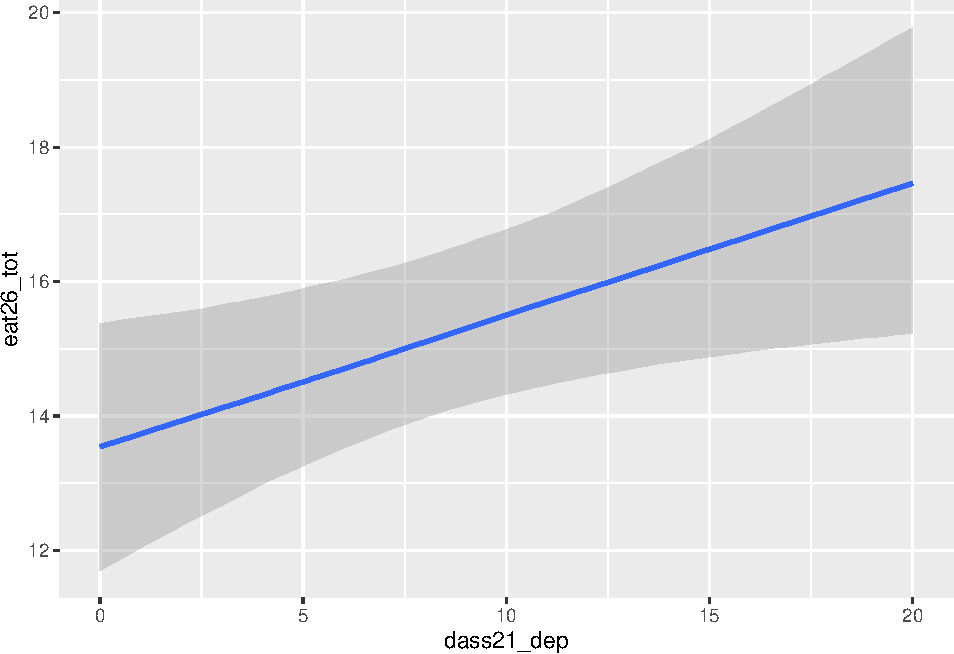
\includegraphics{050_quest_groups_files/figure-latex/unnamed-chunk-2-7.pdf}

\begin{Shaded}
\begin{Highlighting}[]
\NormalTok{m4a }\OtherTok{\textless{}{-}} \FunctionTok{brm}\NormalTok{(}
\NormalTok{  eat26\_tot }\SpecialCharTok{\textasciitilde{}}\NormalTok{ bmi }\SpecialCharTok{+}\NormalTok{ age }\SpecialCharTok{+}\NormalTok{ (dass21\_anxiety }\SpecialCharTok{+}\NormalTok{ dass21\_dep),}
  \AttributeTok{data =}\NormalTok{ quest\_data3[quest\_data3}\SpecialCharTok{$}\NormalTok{sex }\SpecialCharTok{==} \StringTok{"Femmina"} \SpecialCharTok{\&}\NormalTok{ quest\_data3}\SpecialCharTok{$}\NormalTok{is\_patient }\SpecialCharTok{==} \DecValTok{0}\NormalTok{, ], }
  \CommentTok{\# prior = prior\_ma,}
  \AttributeTok{family =} \FunctionTok{skew\_normal}\NormalTok{(),}
  \AttributeTok{control =} \FunctionTok{list}\NormalTok{(}\AttributeTok{adapt\_delta =} \FloatTok{0.98}\NormalTok{),}
  \AttributeTok{iter =} \DecValTok{4000}\NormalTok{,}
  \AttributeTok{cores =} \DecValTok{6}\NormalTok{,}
  \AttributeTok{backend =} \StringTok{"cmdstan"}
\NormalTok{)}
\end{Highlighting}
\end{Shaded}

\begin{verbatim}
## Warning: Rows containing NAs were excluded from the model.
\end{verbatim}

\begin{verbatim}
## Start sampling
\end{verbatim}

\begin{verbatim}
## Running MCMC with 4 chains, at most 6 in parallel...
\end{verbatim}

\begin{verbatim}
## Chain 1 Rejecting initial value:
\end{verbatim}

\begin{verbatim}
## Chain 1   Log probability evaluates to log(0), i.e. negative infinity.
\end{verbatim}

\begin{verbatim}
## Chain 1   Stan can't start sampling from this initial value.
\end{verbatim}

\begin{verbatim}
## Chain 1 Iteration:    1 / 4000 [  0%]  (Warmup)
\end{verbatim}

\begin{verbatim}
## Chain 2 Rejecting initial value:
\end{verbatim}

\begin{verbatim}
## Chain 2   Log probability evaluates to log(0), i.e. negative infinity.
\end{verbatim}

\begin{verbatim}
## Chain 2   Stan can't start sampling from this initial value.
\end{verbatim}

\begin{verbatim}
## Chain 2 Iteration:    1 / 4000 [  0%]  (Warmup)
\end{verbatim}

\begin{verbatim}
## Chain 3 Rejecting initial value:
\end{verbatim}

\begin{verbatim}
## Chain 3   Log probability evaluates to log(0), i.e. negative infinity.
\end{verbatim}

\begin{verbatim}
## Chain 3   Stan can't start sampling from this initial value.
\end{verbatim}

\begin{verbatim}
## Chain 3 Rejecting initial value:
\end{verbatim}

\begin{verbatim}
## Chain 3   Log probability evaluates to log(0), i.e. negative infinity.
\end{verbatim}

\begin{verbatim}
## Chain 3   Stan can't start sampling from this initial value.
\end{verbatim}

\begin{verbatim}
## Chain 3 Iteration:    1 / 4000 [  0%]  (Warmup) 
## Chain 4 Iteration:    1 / 4000 [  0%]  (Warmup) 
## Chain 1 Iteration:  100 / 4000 [  2%]  (Warmup) 
## Chain 1 Iteration:  200 / 4000 [  5%]  (Warmup) 
## Chain 2 Iteration:  100 / 4000 [  2%]  (Warmup) 
## Chain 2 Iteration:  200 / 4000 [  5%]  (Warmup) 
## Chain 3 Iteration:  100 / 4000 [  2%]  (Warmup) 
## Chain 3 Iteration:  200 / 4000 [  5%]  (Warmup) 
## Chain 4 Iteration:  100 / 4000 [  2%]  (Warmup) 
## Chain 4 Iteration:  200 / 4000 [  5%]  (Warmup) 
## Chain 4 Iteration:  300 / 4000 [  7%]  (Warmup) 
## Chain 1 Iteration:  300 / 4000 [  7%]  (Warmup) 
## Chain 1 Iteration:  400 / 4000 [ 10%]  (Warmup) 
## Chain 1 Iteration:  500 / 4000 [ 12%]  (Warmup) 
## Chain 2 Iteration:  300 / 4000 [  7%]  (Warmup) 
## Chain 2 Iteration:  400 / 4000 [ 10%]  (Warmup) 
## Chain 2 Iteration:  500 / 4000 [ 12%]  (Warmup) 
## Chain 3 Iteration:  300 / 4000 [  7%]  (Warmup) 
## Chain 3 Iteration:  400 / 4000 [ 10%]  (Warmup) 
## Chain 3 Iteration:  500 / 4000 [ 12%]  (Warmup) 
## Chain 4 Iteration:  400 / 4000 [ 10%]  (Warmup) 
## Chain 4 Iteration:  500 / 4000 [ 12%]  (Warmup) 
## Chain 4 Iteration:  600 / 4000 [ 15%]  (Warmup) 
## Chain 1 Iteration:  600 / 4000 [ 15%]  (Warmup) 
## Chain 1 Iteration:  700 / 4000 [ 17%]  (Warmup) 
## Chain 1 Iteration:  800 / 4000 [ 20%]  (Warmup) 
## Chain 2 Iteration:  600 / 4000 [ 15%]  (Warmup) 
## Chain 2 Iteration:  700 / 4000 [ 17%]  (Warmup) 
## Chain 2 Iteration:  800 / 4000 [ 20%]  (Warmup) 
## Chain 3 Iteration:  600 / 4000 [ 15%]  (Warmup) 
## Chain 3 Iteration:  700 / 4000 [ 17%]  (Warmup) 
## Chain 3 Iteration:  800 / 4000 [ 20%]  (Warmup) 
## Chain 4 Iteration:  700 / 4000 [ 17%]  (Warmup) 
## Chain 4 Iteration:  800 / 4000 [ 20%]  (Warmup) 
## Chain 4 Iteration:  900 / 4000 [ 22%]  (Warmup) 
## Chain 1 Iteration:  900 / 4000 [ 22%]  (Warmup) 
## Chain 1 Iteration: 1000 / 4000 [ 25%]  (Warmup) 
## Chain 1 Iteration: 1100 / 4000 [ 27%]  (Warmup) 
## Chain 1 Iteration: 1200 / 4000 [ 30%]  (Warmup) 
## Chain 2 Iteration:  900 / 4000 [ 22%]  (Warmup) 
## Chain 2 Iteration: 1000 / 4000 [ 25%]  (Warmup) 
## Chain 2 Iteration: 1100 / 4000 [ 27%]  (Warmup) 
## Chain 2 Iteration: 1200 / 4000 [ 30%]  (Warmup) 
## Chain 3 Iteration:  900 / 4000 [ 22%]  (Warmup) 
## Chain 3 Iteration: 1000 / 4000 [ 25%]  (Warmup) 
## Chain 3 Iteration: 1100 / 4000 [ 27%]  (Warmup) 
## Chain 4 Iteration: 1000 / 4000 [ 25%]  (Warmup) 
## Chain 4 Iteration: 1100 / 4000 [ 27%]  (Warmup) 
## Chain 4 Iteration: 1200 / 4000 [ 30%]  (Warmup) 
## Chain 1 Iteration: 1300 / 4000 [ 32%]  (Warmup) 
## Chain 1 Iteration: 1400 / 4000 [ 35%]  (Warmup) 
## Chain 2 Iteration: 1300 / 4000 [ 32%]  (Warmup) 
## Chain 2 Iteration: 1400 / 4000 [ 35%]  (Warmup) 
## Chain 2 Iteration: 1500 / 4000 [ 37%]  (Warmup) 
## Chain 3 Iteration: 1200 / 4000 [ 30%]  (Warmup) 
## Chain 3 Iteration: 1300 / 4000 [ 32%]  (Warmup) 
## Chain 3 Iteration: 1400 / 4000 [ 35%]  (Warmup) 
## Chain 4 Iteration: 1300 / 4000 [ 32%]  (Warmup) 
## Chain 4 Iteration: 1400 / 4000 [ 35%]  (Warmup) 
## Chain 4 Iteration: 1500 / 4000 [ 37%]  (Warmup) 
## Chain 1 Iteration: 1500 / 4000 [ 37%]  (Warmup) 
## Chain 1 Iteration: 1600 / 4000 [ 40%]  (Warmup) 
## Chain 1 Iteration: 1700 / 4000 [ 42%]  (Warmup) 
## Chain 1 Iteration: 1800 / 4000 [ 45%]  (Warmup) 
## Chain 2 Iteration: 1600 / 4000 [ 40%]  (Warmup) 
## Chain 2 Iteration: 1700 / 4000 [ 42%]  (Warmup) 
## Chain 2 Iteration: 1800 / 4000 [ 45%]  (Warmup) 
## Chain 3 Iteration: 1500 / 4000 [ 37%]  (Warmup) 
## Chain 3 Iteration: 1600 / 4000 [ 40%]  (Warmup) 
## Chain 3 Iteration: 1700 / 4000 [ 42%]  (Warmup) 
## Chain 4 Iteration: 1600 / 4000 [ 40%]  (Warmup) 
## Chain 4 Iteration: 1700 / 4000 [ 42%]  (Warmup) 
## Chain 4 Iteration: 1800 / 4000 [ 45%]  (Warmup) 
## Chain 1 Iteration: 1900 / 4000 [ 47%]  (Warmup) 
## Chain 1 Iteration: 2000 / 4000 [ 50%]  (Warmup) 
## Chain 1 Iteration: 2001 / 4000 [ 50%]  (Sampling) 
## Chain 2 Iteration: 1900 / 4000 [ 47%]  (Warmup) 
## Chain 2 Iteration: 2000 / 4000 [ 50%]  (Warmup) 
## Chain 2 Iteration: 2001 / 4000 [ 50%]  (Sampling) 
## Chain 2 Iteration: 2100 / 4000 [ 52%]  (Sampling) 
## Chain 3 Iteration: 1800 / 4000 [ 45%]  (Warmup) 
## Chain 3 Iteration: 1900 / 4000 [ 47%]  (Warmup) 
## Chain 3 Iteration: 2000 / 4000 [ 50%]  (Warmup) 
## Chain 3 Iteration: 2001 / 4000 [ 50%]  (Sampling) 
## Chain 4 Iteration: 1900 / 4000 [ 47%]  (Warmup) 
## Chain 4 Iteration: 2000 / 4000 [ 50%]  (Warmup) 
## Chain 4 Iteration: 2001 / 4000 [ 50%]  (Sampling) 
## Chain 4 Iteration: 2100 / 4000 [ 52%]  (Sampling) 
## Chain 4 Iteration: 2200 / 4000 [ 55%]  (Sampling) 
## Chain 1 Iteration: 2100 / 4000 [ 52%]  (Sampling) 
## Chain 1 Iteration: 2200 / 4000 [ 55%]  (Sampling) 
## Chain 1 Iteration: 2300 / 4000 [ 57%]  (Sampling) 
## Chain 2 Iteration: 2200 / 4000 [ 55%]  (Sampling) 
## Chain 2 Iteration: 2300 / 4000 [ 57%]  (Sampling) 
## Chain 3 Iteration: 2100 / 4000 [ 52%]  (Sampling) 
## Chain 3 Iteration: 2200 / 4000 [ 55%]  (Sampling) 
## Chain 4 Iteration: 2300 / 4000 [ 57%]  (Sampling) 
## Chain 4 Iteration: 2400 / 4000 [ 60%]  (Sampling) 
## Chain 4 Iteration: 2500 / 4000 [ 62%]  (Sampling) 
## Chain 1 Iteration: 2400 / 4000 [ 60%]  (Sampling) 
## Chain 1 Iteration: 2500 / 4000 [ 62%]  (Sampling) 
## Chain 2 Iteration: 2400 / 4000 [ 60%]  (Sampling) 
## Chain 2 Iteration: 2500 / 4000 [ 62%]  (Sampling) 
## Chain 2 Iteration: 2600 / 4000 [ 65%]  (Sampling) 
## Chain 3 Iteration: 2300 / 4000 [ 57%]  (Sampling) 
## Chain 3 Iteration: 2400 / 4000 [ 60%]  (Sampling) 
## Chain 4 Iteration: 2600 / 4000 [ 65%]  (Sampling) 
## Chain 4 Iteration: 2700 / 4000 [ 67%]  (Sampling) 
## Chain 4 Iteration: 2800 / 4000 [ 70%]  (Sampling) 
## Chain 4 Iteration: 2900 / 4000 [ 72%]  (Sampling) 
## Chain 1 Iteration: 2600 / 4000 [ 65%]  (Sampling) 
## Chain 1 Iteration: 2700 / 4000 [ 67%]  (Sampling) 
## Chain 2 Iteration: 2700 / 4000 [ 67%]  (Sampling) 
## Chain 2 Iteration: 2800 / 4000 [ 70%]  (Sampling) 
## Chain 3 Iteration: 2500 / 4000 [ 62%]  (Sampling) 
## Chain 3 Iteration: 2600 / 4000 [ 65%]  (Sampling) 
## Chain 3 Iteration: 2700 / 4000 [ 67%]  (Sampling) 
## Chain 4 Iteration: 3000 / 4000 [ 75%]  (Sampling) 
## Chain 4 Iteration: 3100 / 4000 [ 77%]  (Sampling) 
## Chain 4 Iteration: 3200 / 4000 [ 80%]  (Sampling) 
## Chain 1 Iteration: 2800 / 4000 [ 70%]  (Sampling) 
## Chain 1 Iteration: 2900 / 4000 [ 72%]  (Sampling) 
## Chain 1 Iteration: 3000 / 4000 [ 75%]  (Sampling) 
## Chain 2 Iteration: 2900 / 4000 [ 72%]  (Sampling) 
## Chain 2 Iteration: 3000 / 4000 [ 75%]  (Sampling) 
## Chain 2 Iteration: 3100 / 4000 [ 77%]  (Sampling) 
## Chain 3 Iteration: 2800 / 4000 [ 70%]  (Sampling) 
## Chain 3 Iteration: 2900 / 4000 [ 72%]  (Sampling) 
## Chain 4 Iteration: 3300 / 4000 [ 82%]  (Sampling) 
## Chain 4 Iteration: 3400 / 4000 [ 85%]  (Sampling) 
## Chain 4 Iteration: 3500 / 4000 [ 87%]  (Sampling) 
## Chain 1 Iteration: 3100 / 4000 [ 77%]  (Sampling) 
## Chain 1 Iteration: 3200 / 4000 [ 80%]  (Sampling) 
## Chain 2 Iteration: 3200 / 4000 [ 80%]  (Sampling) 
## Chain 2 Iteration: 3300 / 4000 [ 82%]  (Sampling) 
## Chain 3 Iteration: 3000 / 4000 [ 75%]  (Sampling) 
## Chain 3 Iteration: 3100 / 4000 [ 77%]  (Sampling) 
## Chain 4 Iteration: 3600 / 4000 [ 90%]  (Sampling) 
## Chain 4 Iteration: 3700 / 4000 [ 92%]  (Sampling) 
## Chain 4 Iteration: 3800 / 4000 [ 95%]  (Sampling) 
## Chain 4 Iteration: 3900 / 4000 [ 97%]  (Sampling) 
## Chain 1 Iteration: 3300 / 4000 [ 82%]  (Sampling) 
## Chain 1 Iteration: 3400 / 4000 [ 85%]  (Sampling) 
## Chain 2 Iteration: 3400 / 4000 [ 85%]  (Sampling) 
## Chain 2 Iteration: 3500 / 4000 [ 87%]  (Sampling) 
## Chain 2 Iteration: 3600 / 4000 [ 90%]  (Sampling) 
## Chain 3 Iteration: 3200 / 4000 [ 80%]  (Sampling) 
## Chain 3 Iteration: 3300 / 4000 [ 82%]  (Sampling) 
## Chain 4 Iteration: 4000 / 4000 [100%]  (Sampling) 
## Chain 4 finished in 1.4 seconds.
## Chain 1 Iteration: 3500 / 4000 [ 87%]  (Sampling) 
## Chain 1 Iteration: 3600 / 4000 [ 90%]  (Sampling) 
## Chain 1 Iteration: 3700 / 4000 [ 92%]  (Sampling) 
## Chain 2 Iteration: 3700 / 4000 [ 92%]  (Sampling) 
## Chain 2 Iteration: 3800 / 4000 [ 95%]  (Sampling) 
## Chain 2 Iteration: 3900 / 4000 [ 97%]  (Sampling) 
## Chain 3 Iteration: 3400 / 4000 [ 85%]  (Sampling) 
## Chain 3 Iteration: 3500 / 4000 [ 87%]  (Sampling) 
## Chain 3 Iteration: 3600 / 4000 [ 90%]  (Sampling) 
## Chain 1 Iteration: 3800 / 4000 [ 95%]  (Sampling) 
## Chain 1 Iteration: 3900 / 4000 [ 97%]  (Sampling) 
## Chain 2 Iteration: 4000 / 4000 [100%]  (Sampling) 
## Chain 3 Iteration: 3700 / 4000 [ 92%]  (Sampling) 
## Chain 3 Iteration: 3800 / 4000 [ 95%]  (Sampling) 
## Chain 2 finished in 1.6 seconds.
## Chain 1 Iteration: 4000 / 4000 [100%]  (Sampling) 
## Chain 3 Iteration: 3900 / 4000 [ 97%]  (Sampling) 
## Chain 3 Iteration: 4000 / 4000 [100%]  (Sampling) 
## Chain 1 finished in 1.7 seconds.
## Chain 3 finished in 1.8 seconds.
## 
## All 4 chains finished successfully.
## Mean chain execution time: 1.6 seconds.
## Total execution time: 2.0 seconds.
\end{verbatim}

\begin{Shaded}
\begin{Highlighting}[]
\FunctionTok{summary}\NormalTok{(m4a)}
\end{Highlighting}
\end{Shaded}

\begin{verbatim}
##  Family: skew_normal 
##   Links: mu = identity; sigma = identity; alpha = identity 
## Formula: eat26_tot ~ bmi + age + (dass21_anxiety + dass21_dep) 
##    Data: quest_data3[quest_data3$sex == "Femmina" & quest_d (Number of observations: 206) 
## Samples: 4 chains, each with iter = 4000; warmup = 2000; thin = 1;
##          total post-warmup samples = 8000
## 
## Population-Level Effects: 
##                Estimate Est.Error l-95% CI u-95% CI Rhat Bulk_ESS Tail_ESS
## Intercept         11.12      3.43     4.54    18.09 1.00     6304     5028
## bmi                0.10      0.12    -0.14     0.33 1.00     5903     4785
## age               -0.08      0.10    -0.29     0.09 1.00     6683     4189
## dass21_anxiety    -0.02      0.09    -0.20     0.14 1.00     5557     5711
## dass21_dep         0.18      0.08     0.03     0.34 1.00     5173     5149
## 
## Family Specific Parameters: 
##       Estimate Est.Error l-95% CI u-95% CI Rhat Bulk_ESS Tail_ESS
## sigma     7.75      0.39     7.04     8.55 1.00     4893     5205
## alpha    10.62      2.17     6.90    15.20 1.00     5678     4357
## 
## Samples were drawn using sample(hmc). For each parameter, Bulk_ESS
## and Tail_ESS are effective sample size measures, and Rhat is the potential
## scale reduction factor on split chains (at convergence, Rhat = 1).
\end{verbatim}

\begin{Shaded}
\begin{Highlighting}[]
\FunctionTok{plot}\NormalTok{(}\FunctionTok{conditional\_effects}\NormalTok{(m4a, }\StringTok{"dass21\_dep"}\NormalTok{))}
\end{Highlighting}
\end{Shaded}

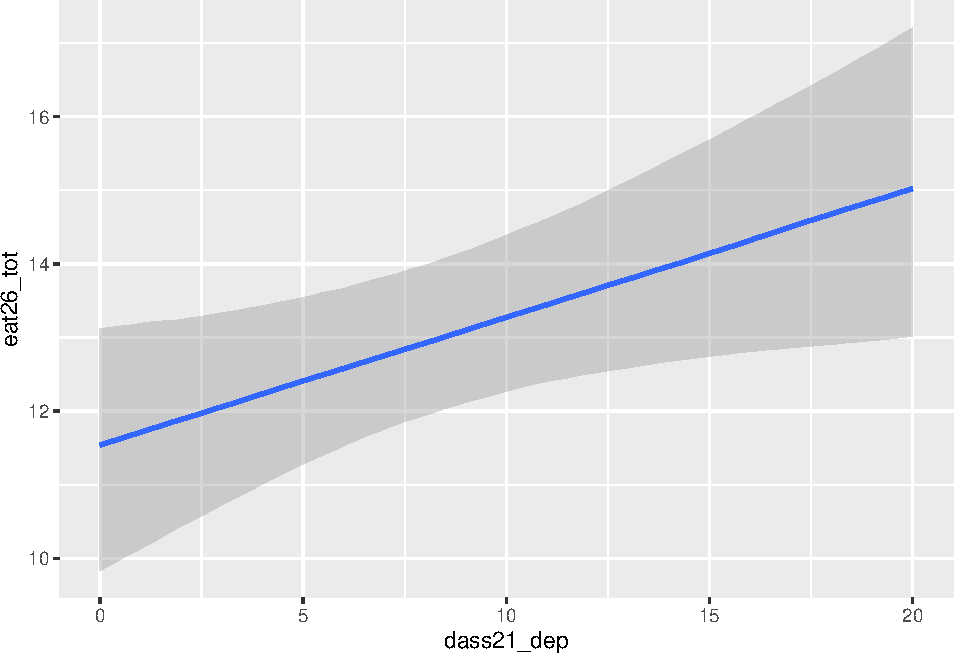
\includegraphics{050_quest_groups_files/figure-latex/unnamed-chunk-2-8.pdf}

\begin{Shaded}
\begin{Highlighting}[]
\NormalTok{m5 }\OtherTok{\textless{}{-}} \FunctionTok{brm}\NormalTok{(}
\NormalTok{  eat26\_tot }\SpecialCharTok{\textasciitilde{}}\NormalTok{ bmi }\SpecialCharTok{+}\NormalTok{ age }\SpecialCharTok{+}\NormalTok{ (dass21\_anxiety }\SpecialCharTok{+}\NormalTok{ dass21\_dep),}
  \AttributeTok{data =}\NormalTok{ quest\_data3[quest\_data3}\SpecialCharTok{$}\NormalTok{sex }\SpecialCharTok{==} \StringTok{"Maschio"}\NormalTok{, ], }
  \CommentTok{\# prior = prior\_ma,}
  \AttributeTok{family =} \FunctionTok{skew\_normal}\NormalTok{(),}
  \AttributeTok{control =} \FunctionTok{list}\NormalTok{(}\AttributeTok{adapt\_delta =} \FloatTok{0.98}\NormalTok{),}
  \AttributeTok{iter =} \DecValTok{4000}\NormalTok{,}
  \AttributeTok{cores =} \DecValTok{6}\NormalTok{,}
  \AttributeTok{backend =} \StringTok{"cmdstan"}
\NormalTok{)}
\end{Highlighting}
\end{Shaded}

\begin{verbatim}
## Start sampling
\end{verbatim}

\begin{verbatim}
## Running MCMC with 4 chains, at most 6 in parallel...
## 
## Chain 1 Iteration:    1 / 4000 [  0%]  (Warmup) 
## Chain 1 Iteration:  100 / 4000 [  2%]  (Warmup) 
## Chain 1 Iteration:  200 / 4000 [  5%]  (Warmup) 
## Chain 1 Iteration:  300 / 4000 [  7%]  (Warmup) 
## Chain 1 Iteration:  400 / 4000 [ 10%]  (Warmup) 
## Chain 1 Iteration:  500 / 4000 [ 12%]  (Warmup) 
## Chain 2 Iteration:    1 / 4000 [  0%]  (Warmup) 
## Chain 2 Iteration:  100 / 4000 [  2%]  (Warmup) 
## Chain 2 Iteration:  200 / 4000 [  5%]  (Warmup) 
## Chain 2 Iteration:  300 / 4000 [  7%]  (Warmup) 
## Chain 2 Iteration:  400 / 4000 [ 10%]  (Warmup) 
## Chain 2 Iteration:  500 / 4000 [ 12%]  (Warmup) 
## Chain 2 Iteration:  600 / 4000 [ 15%]  (Warmup) 
## Chain 3 Iteration:    1 / 4000 [  0%]  (Warmup) 
## Chain 3 Iteration:  100 / 4000 [  2%]  (Warmup) 
## Chain 3 Iteration:  200 / 4000 [  5%]  (Warmup) 
## Chain 3 Iteration:  300 / 4000 [  7%]  (Warmup) 
## Chain 3 Iteration:  400 / 4000 [ 10%]  (Warmup) 
## Chain 3 Iteration:  500 / 4000 [ 12%]  (Warmup) 
## Chain 3 Iteration:  600 / 4000 [ 15%]  (Warmup) 
## Chain 3 Iteration:  700 / 4000 [ 17%]  (Warmup) 
## Chain 4 Iteration:    1 / 4000 [  0%]  (Warmup) 
## Chain 4 Iteration:  100 / 4000 [  2%]  (Warmup) 
## Chain 4 Iteration:  200 / 4000 [  5%]  (Warmup) 
## Chain 4 Iteration:  300 / 4000 [  7%]  (Warmup) 
## Chain 4 Iteration:  400 / 4000 [ 10%]  (Warmup) 
## Chain 4 Iteration:  500 / 4000 [ 12%]  (Warmup) 
## Chain 4 Iteration:  600 / 4000 [ 15%]  (Warmup) 
## Chain 4 Iteration:  700 / 4000 [ 17%]  (Warmup) 
## Chain 4 Iteration:  800 / 4000 [ 20%]  (Warmup) 
## Chain 1 Iteration:  600 / 4000 [ 15%]  (Warmup) 
## Chain 1 Iteration:  700 / 4000 [ 17%]  (Warmup) 
## Chain 1 Iteration:  800 / 4000 [ 20%]  (Warmup) 
## Chain 1 Iteration:  900 / 4000 [ 22%]  (Warmup) 
## Chain 1 Iteration: 1000 / 4000 [ 25%]  (Warmup) 
## Chain 1 Iteration: 1100 / 4000 [ 27%]  (Warmup) 
## Chain 1 Iteration: 1200 / 4000 [ 30%]  (Warmup) 
## Chain 1 Iteration: 1300 / 4000 [ 32%]  (Warmup) 
## Chain 1 Iteration: 1400 / 4000 [ 35%]  (Warmup) 
## Chain 1 Iteration: 1500 / 4000 [ 37%]  (Warmup) 
## Chain 1 Iteration: 1600 / 4000 [ 40%]  (Warmup) 
## Chain 1 Iteration: 1700 / 4000 [ 42%]  (Warmup) 
## Chain 1 Iteration: 1800 / 4000 [ 45%]  (Warmup) 
## Chain 1 Iteration: 1900 / 4000 [ 47%]  (Warmup) 
## Chain 1 Iteration: 2000 / 4000 [ 50%]  (Warmup) 
## Chain 1 Iteration: 2001 / 4000 [ 50%]  (Sampling) 
## Chain 2 Iteration:  700 / 4000 [ 17%]  (Warmup) 
## Chain 2 Iteration:  800 / 4000 [ 20%]  (Warmup) 
## Chain 2 Iteration:  900 / 4000 [ 22%]  (Warmup) 
## Chain 2 Iteration: 1000 / 4000 [ 25%]  (Warmup) 
## Chain 2 Iteration: 1100 / 4000 [ 27%]  (Warmup) 
## Chain 2 Iteration: 1200 / 4000 [ 30%]  (Warmup) 
## Chain 2 Iteration: 1300 / 4000 [ 32%]  (Warmup) 
## Chain 2 Iteration: 1400 / 4000 [ 35%]  (Warmup) 
## Chain 2 Iteration: 1500 / 4000 [ 37%]  (Warmup) 
## Chain 2 Iteration: 1600 / 4000 [ 40%]  (Warmup) 
## Chain 2 Iteration: 1700 / 4000 [ 42%]  (Warmup) 
## Chain 2 Iteration: 1800 / 4000 [ 45%]  (Warmup) 
## Chain 2 Iteration: 1900 / 4000 [ 47%]  (Warmup) 
## Chain 2 Iteration: 2000 / 4000 [ 50%]  (Warmup) 
## Chain 2 Iteration: 2001 / 4000 [ 50%]  (Sampling) 
## Chain 3 Iteration:  800 / 4000 [ 20%]  (Warmup) 
## Chain 3 Iteration:  900 / 4000 [ 22%]  (Warmup) 
## Chain 3 Iteration: 1000 / 4000 [ 25%]  (Warmup) 
## Chain 3 Iteration: 1100 / 4000 [ 27%]  (Warmup) 
## Chain 3 Iteration: 1200 / 4000 [ 30%]  (Warmup) 
## Chain 3 Iteration: 1300 / 4000 [ 32%]  (Warmup) 
## Chain 3 Iteration: 1400 / 4000 [ 35%]  (Warmup) 
## Chain 3 Iteration: 1500 / 4000 [ 37%]  (Warmup) 
## Chain 3 Iteration: 1600 / 4000 [ 40%]  (Warmup) 
## Chain 3 Iteration: 1700 / 4000 [ 42%]  (Warmup) 
## Chain 3 Iteration: 1800 / 4000 [ 45%]  (Warmup) 
## Chain 3 Iteration: 1900 / 4000 [ 47%]  (Warmup) 
## Chain 3 Iteration: 2000 / 4000 [ 50%]  (Warmup) 
## Chain 3 Iteration: 2001 / 4000 [ 50%]  (Sampling) 
## Chain 4 Iteration:  900 / 4000 [ 22%]  (Warmup) 
## Chain 4 Iteration: 1000 / 4000 [ 25%]  (Warmup) 
## Chain 4 Iteration: 1100 / 4000 [ 27%]  (Warmup) 
## Chain 4 Iteration: 1200 / 4000 [ 30%]  (Warmup) 
## Chain 4 Iteration: 1300 / 4000 [ 32%]  (Warmup) 
## Chain 4 Iteration: 1400 / 4000 [ 35%]  (Warmup) 
## Chain 4 Iteration: 1500 / 4000 [ 37%]  (Warmup) 
## Chain 4 Iteration: 1600 / 4000 [ 40%]  (Warmup) 
## Chain 4 Iteration: 1700 / 4000 [ 42%]  (Warmup) 
## Chain 4 Iteration: 1800 / 4000 [ 45%]  (Warmup) 
## Chain 4 Iteration: 1900 / 4000 [ 47%]  (Warmup) 
## Chain 4 Iteration: 2000 / 4000 [ 50%]  (Warmup) 
## Chain 4 Iteration: 2001 / 4000 [ 50%]  (Sampling) 
## Chain 4 Iteration: 2100 / 4000 [ 52%]  (Sampling) 
## Chain 1 Iteration: 2100 / 4000 [ 52%]  (Sampling) 
## Chain 1 Iteration: 2200 / 4000 [ 55%]  (Sampling) 
## Chain 1 Iteration: 2300 / 4000 [ 57%]  (Sampling) 
## Chain 1 Iteration: 2400 / 4000 [ 60%]  (Sampling) 
## Chain 1 Iteration: 2500 / 4000 [ 62%]  (Sampling) 
## Chain 1 Iteration: 2600 / 4000 [ 65%]  (Sampling) 
## Chain 1 Iteration: 2700 / 4000 [ 67%]  (Sampling) 
## Chain 1 Iteration: 2800 / 4000 [ 70%]  (Sampling) 
## Chain 1 Iteration: 2900 / 4000 [ 72%]  (Sampling) 
## Chain 1 Iteration: 3000 / 4000 [ 75%]  (Sampling) 
## Chain 1 Iteration: 3100 / 4000 [ 77%]  (Sampling) 
## Chain 1 Iteration: 3200 / 4000 [ 80%]  (Sampling) 
## Chain 2 Iteration: 2100 / 4000 [ 52%]  (Sampling) 
## Chain 2 Iteration: 2200 / 4000 [ 55%]  (Sampling) 
## Chain 2 Iteration: 2300 / 4000 [ 57%]  (Sampling) 
## Chain 2 Iteration: 2400 / 4000 [ 60%]  (Sampling) 
## Chain 2 Iteration: 2500 / 4000 [ 62%]  (Sampling) 
## Chain 2 Iteration: 2600 / 4000 [ 65%]  (Sampling) 
## Chain 2 Iteration: 2700 / 4000 [ 67%]  (Sampling) 
## Chain 2 Iteration: 2800 / 4000 [ 70%]  (Sampling) 
## Chain 2 Iteration: 2900 / 4000 [ 72%]  (Sampling) 
## Chain 2 Iteration: 3000 / 4000 [ 75%]  (Sampling) 
## Chain 2 Iteration: 3100 / 4000 [ 77%]  (Sampling) 
## Chain 2 Iteration: 3200 / 4000 [ 80%]  (Sampling) 
## Chain 3 Iteration: 2100 / 4000 [ 52%]  (Sampling) 
## Chain 3 Iteration: 2200 / 4000 [ 55%]  (Sampling) 
## Chain 3 Iteration: 2300 / 4000 [ 57%]  (Sampling) 
## Chain 3 Iteration: 2400 / 4000 [ 60%]  (Sampling) 
## Chain 3 Iteration: 2500 / 4000 [ 62%]  (Sampling) 
## Chain 3 Iteration: 2600 / 4000 [ 65%]  (Sampling) 
## Chain 3 Iteration: 2700 / 4000 [ 67%]  (Sampling) 
## Chain 3 Iteration: 2800 / 4000 [ 70%]  (Sampling) 
## Chain 3 Iteration: 2900 / 4000 [ 72%]  (Sampling) 
## Chain 4 Iteration: 2200 / 4000 [ 55%]  (Sampling) 
## Chain 4 Iteration: 2300 / 4000 [ 57%]  (Sampling) 
## Chain 4 Iteration: 2400 / 4000 [ 60%]  (Sampling) 
## Chain 4 Iteration: 2500 / 4000 [ 62%]  (Sampling) 
## Chain 4 Iteration: 2600 / 4000 [ 65%]  (Sampling) 
## Chain 4 Iteration: 2700 / 4000 [ 67%]  (Sampling) 
## Chain 4 Iteration: 2800 / 4000 [ 70%]  (Sampling) 
## Chain 4 Iteration: 2900 / 4000 [ 72%]  (Sampling) 
## Chain 4 Iteration: 3000 / 4000 [ 75%]  (Sampling) 
## Chain 1 Iteration: 3300 / 4000 [ 82%]  (Sampling) 
## Chain 1 Iteration: 3400 / 4000 [ 85%]  (Sampling) 
## Chain 1 Iteration: 3500 / 4000 [ 87%]  (Sampling) 
## Chain 1 Iteration: 3600 / 4000 [ 90%]  (Sampling) 
## Chain 1 Iteration: 3700 / 4000 [ 92%]  (Sampling) 
## Chain 1 Iteration: 3800 / 4000 [ 95%]  (Sampling) 
## Chain 1 Iteration: 3900 / 4000 [ 97%]  (Sampling) 
## Chain 1 Iteration: 4000 / 4000 [100%]  (Sampling) 
## Chain 2 Iteration: 3300 / 4000 [ 82%]  (Sampling) 
## Chain 2 Iteration: 3400 / 4000 [ 85%]  (Sampling) 
## Chain 2 Iteration: 3500 / 4000 [ 87%]  (Sampling) 
## Chain 2 Iteration: 3600 / 4000 [ 90%]  (Sampling) 
## Chain 2 Iteration: 3700 / 4000 [ 92%]  (Sampling) 
## Chain 2 Iteration: 3800 / 4000 [ 95%]  (Sampling) 
## Chain 2 Iteration: 3900 / 4000 [ 97%]  (Sampling) 
## Chain 2 Iteration: 4000 / 4000 [100%]  (Sampling) 
## Chain 3 Iteration: 3000 / 4000 [ 75%]  (Sampling) 
## Chain 3 Iteration: 3100 / 4000 [ 77%]  (Sampling) 
## Chain 3 Iteration: 3200 / 4000 [ 80%]  (Sampling) 
## Chain 3 Iteration: 3300 / 4000 [ 82%]  (Sampling) 
## Chain 3 Iteration: 3400 / 4000 [ 85%]  (Sampling) 
## Chain 3 Iteration: 3500 / 4000 [ 87%]  (Sampling) 
## Chain 3 Iteration: 3600 / 4000 [ 90%]  (Sampling) 
## Chain 3 Iteration: 3700 / 4000 [ 92%]  (Sampling) 
## Chain 3 Iteration: 3800 / 4000 [ 95%]  (Sampling) 
## Chain 4 Iteration: 3100 / 4000 [ 77%]  (Sampling) 
## Chain 4 Iteration: 3200 / 4000 [ 80%]  (Sampling) 
## Chain 4 Iteration: 3300 / 4000 [ 82%]  (Sampling) 
## Chain 4 Iteration: 3400 / 4000 [ 85%]  (Sampling) 
## Chain 4 Iteration: 3500 / 4000 [ 87%]  (Sampling) 
## Chain 4 Iteration: 3600 / 4000 [ 90%]  (Sampling) 
## Chain 4 Iteration: 3700 / 4000 [ 92%]  (Sampling) 
## Chain 4 Iteration: 3800 / 4000 [ 95%]  (Sampling) 
## Chain 4 Iteration: 3900 / 4000 [ 97%]  (Sampling) 
## Chain 1 finished in 0.4 seconds.
## Chain 2 finished in 0.4 seconds.
## Chain 3 Iteration: 3900 / 4000 [ 97%]  (Sampling) 
## Chain 3 Iteration: 4000 / 4000 [100%]  (Sampling) 
## Chain 4 Iteration: 4000 / 4000 [100%]  (Sampling) 
## Chain 3 finished in 0.5 seconds.
## Chain 4 finished in 0.5 seconds.
## 
## All 4 chains finished successfully.
## Mean chain execution time: 0.4 seconds.
## Total execution time: 0.7 seconds.
\end{verbatim}

\begin{Shaded}
\begin{Highlighting}[]
\FunctionTok{summary}\NormalTok{(m5)}
\end{Highlighting}
\end{Shaded}

\begin{verbatim}
##  Family: skew_normal 
##   Links: mu = identity; sigma = identity; alpha = identity 
## Formula: eat26_tot ~ bmi + age + (dass21_anxiety + dass21_dep) 
##    Data: quest_data3[quest_data3$sex == "Maschio", ] (Number of observations: 40) 
## Samples: 4 chains, each with iter = 4000; warmup = 2000; thin = 1;
##          total post-warmup samples = 8000
## 
## Population-Level Effects: 
##                Estimate Est.Error l-95% CI u-95% CI Rhat Bulk_ESS Tail_ESS
## Intercept         25.46      8.92     7.59    42.57 1.00     5497     4860
## bmi               -0.66      0.38    -1.44     0.08 1.00     4708     4544
## age               -0.01      0.16    -0.35     0.27 1.00     4968     4316
## dass21_anxiety     0.05      0.35    -0.64     0.75 1.00     5240     4398
## dass21_dep         0.00      0.27    -0.58     0.51 1.00     4552     4385
## 
## Family Specific Parameters: 
##       Estimate Est.Error l-95% CI u-95% CI Rhat Bulk_ESS Tail_ESS
## sigma     8.77      1.05     7.01    11.08 1.00     4430     4709
## alpha     7.09      2.22     3.45    11.99 1.00     5162     4590
## 
## Samples were drawn using sample(hmc). For each parameter, Bulk_ESS
## and Tail_ESS are effective sample size measures, and Rhat is the potential
## scale reduction factor on split chains (at convergence, Rhat = 1).
\end{verbatim}

\begin{Shaded}
\begin{Highlighting}[]
\FunctionTok{plot}\NormalTok{(}\FunctionTok{conditional\_effects}\NormalTok{(m5, }\StringTok{"dass21\_dep"}\NormalTok{))}
\end{Highlighting}
\end{Shaded}

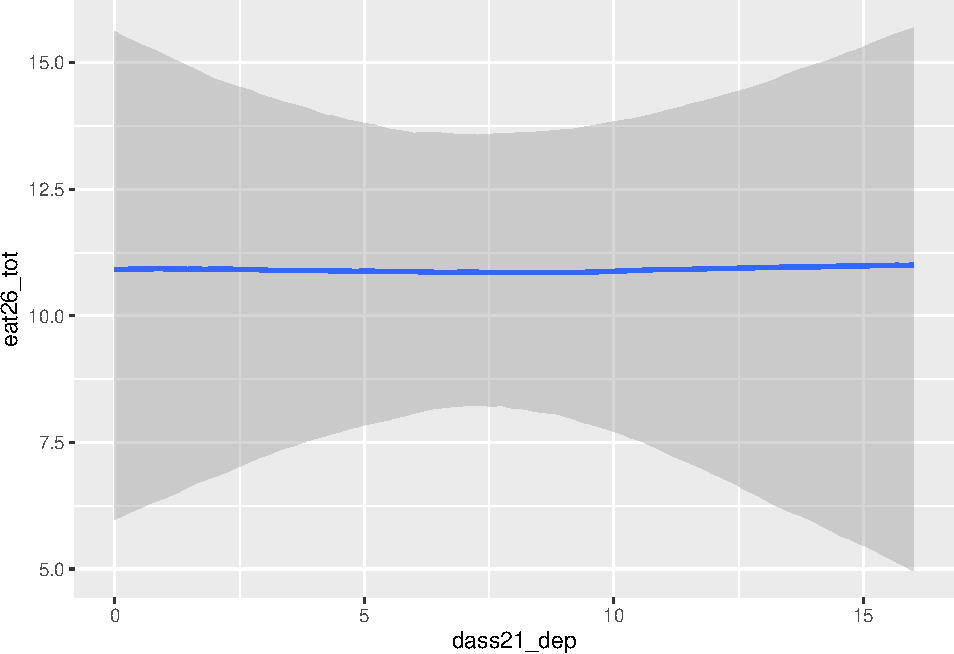
\includegraphics{050_quest_groups_files/figure-latex/unnamed-chunk-2-9.pdf}

\begin{Shaded}
\begin{Highlighting}[]
\NormalTok{quest\_data3 }\SpecialCharTok{\%\textgreater{}\%} 
  \FunctionTok{group\_by}\NormalTok{(sex) }\SpecialCharTok{\%\textgreater{}\%} 
  \FunctionTok{summarise}\NormalTok{(}
    \AttributeTok{avg\_bu =} \FunctionTok{mean}\NormalTok{(bulimia, }\AttributeTok{trim =} \FloatTok{0.1}\NormalTok{, }\AttributeTok{na.rm =} \ConstantTok{TRUE}\NormalTok{),}
    \AttributeTok{avg\_di =} \FunctionTok{mean}\NormalTok{(dieting, }\AttributeTok{trim =} \FloatTok{0.1}\NormalTok{, }\AttributeTok{na.rm =} \ConstantTok{TRUE}\NormalTok{),}
    \AttributeTok{avg\_oc =} \FunctionTok{mean}\NormalTok{(oral\_control, }\AttributeTok{trim =} \FloatTok{0.1}\NormalTok{, }\AttributeTok{na.rm =} \ConstantTok{TRUE}\NormalTok{),}
    \AttributeTok{n =} \FunctionTok{n}\NormalTok{()}
\NormalTok{  )}
\end{Highlighting}
\end{Shaded}

\begin{verbatim}
## # A tibble: 2 x 5
##   sex     avg_bu avg_di avg_oc     n
##   <chr>    <dbl>  <dbl>  <dbl> <int>
## 1 Femmina   4.18   5.28  1.24    244
## 2 Maschio   3.31   2.12  0.969    40
\end{verbatim}

\begin{Shaded}
\begin{Highlighting}[]
\NormalTok{dat }\OtherTok{\textless{}{-}}\NormalTok{ quest\_data2 }\SpecialCharTok{\%\textgreater{}\%} 
\NormalTok{  dplyr}\SpecialCharTok{::}\FunctionTok{filter}\NormalTok{(sex }\SpecialCharTok{!=} \StringTok{"Altro"}\NormalTok{)}

\NormalTok{dat}\SpecialCharTok{$}\NormalTok{is\_patient }\OtherTok{\textless{}{-}} \FunctionTok{factor}\NormalTok{(dat}\SpecialCharTok{$}\NormalTok{is\_patient)}

\NormalTok{m6 }\OtherTok{\textless{}{-}} \FunctionTok{brm}\NormalTok{(}
\NormalTok{  bulimia }\SpecialCharTok{\textasciitilde{}}\NormalTok{ sex,}
  \AttributeTok{data =}\NormalTok{ dat, }
  \CommentTok{\# prior = prior\_ma,}
  \AttributeTok{family =} \FunctionTok{skew\_normal}\NormalTok{(),}
  \AttributeTok{control =} \FunctionTok{list}\NormalTok{(}\AttributeTok{adapt\_delta =} \FloatTok{0.98}\NormalTok{),}
  \AttributeTok{iter =} \DecValTok{4000}\NormalTok{,}
  \AttributeTok{cores =} \DecValTok{6}\NormalTok{,}
  \AttributeTok{backend =} \StringTok{"cmdstan"}
\NormalTok{)}
\end{Highlighting}
\end{Shaded}

\begin{verbatim}
## Warning: Rows containing NAs were excluded from the model.
\end{verbatim}

\begin{verbatim}
## Start sampling
\end{verbatim}

\begin{verbatim}
## Running MCMC with 4 chains, at most 6 in parallel...
## 
## Chain 1 Iteration:    1 / 4000 [  0%]  (Warmup) 
## Chain 2 Iteration:    1 / 4000 [  0%]  (Warmup) 
## Chain 3 Iteration:    1 / 4000 [  0%]  (Warmup) 
## Chain 4 Iteration:    1 / 4000 [  0%]  (Warmup) 
## Chain 4 Iteration:  100 / 4000 [  2%]  (Warmup) 
## Chain 1 Iteration:  100 / 4000 [  2%]  (Warmup) 
## Chain 1 Iteration:  200 / 4000 [  5%]  (Warmup) 
## Chain 2 Iteration:  100 / 4000 [  2%]  (Warmup) 
## Chain 2 Iteration:  200 / 4000 [  5%]  (Warmup) 
## Chain 3 Iteration:  100 / 4000 [  2%]  (Warmup) 
## Chain 4 Iteration:  200 / 4000 [  5%]  (Warmup) 
## Chain 1 Iteration:  300 / 4000 [  7%]  (Warmup) 
## Chain 2 Iteration:  300 / 4000 [  7%]  (Warmup) 
## Chain 2 Iteration:  400 / 4000 [ 10%]  (Warmup) 
## Chain 3 Iteration:  200 / 4000 [  5%]  (Warmup) 
## Chain 3 Iteration:  300 / 4000 [  7%]  (Warmup) 
## Chain 4 Iteration:  300 / 4000 [  7%]  (Warmup) 
## Chain 4 Iteration:  400 / 4000 [ 10%]  (Warmup) 
## Chain 1 Iteration:  400 / 4000 [ 10%]  (Warmup) 
## Chain 2 Iteration:  500 / 4000 [ 12%]  (Warmup) 
## Chain 2 Iteration:  600 / 4000 [ 15%]  (Warmup) 
## Chain 3 Iteration:  400 / 4000 [ 10%]  (Warmup) 
## Chain 3 Iteration:  500 / 4000 [ 12%]  (Warmup) 
## Chain 4 Iteration:  500 / 4000 [ 12%]  (Warmup) 
## Chain 4 Iteration:  600 / 4000 [ 15%]  (Warmup) 
## Chain 1 Iteration:  500 / 4000 [ 12%]  (Warmup) 
## Chain 1 Iteration:  600 / 4000 [ 15%]  (Warmup) 
## Chain 2 Iteration:  700 / 4000 [ 17%]  (Warmup) 
## Chain 2 Iteration:  800 / 4000 [ 20%]  (Warmup) 
## Chain 3 Iteration:  600 / 4000 [ 15%]  (Warmup) 
## Chain 3 Iteration:  700 / 4000 [ 17%]  (Warmup) 
## Chain 4 Iteration:  700 / 4000 [ 17%]  (Warmup) 
## Chain 4 Iteration:  800 / 4000 [ 20%]  (Warmup) 
## Chain 1 Iteration:  700 / 4000 [ 17%]  (Warmup) 
## Chain 1 Iteration:  800 / 4000 [ 20%]  (Warmup) 
## Chain 2 Iteration:  900 / 4000 [ 22%]  (Warmup) 
## Chain 2 Iteration: 1000 / 4000 [ 25%]  (Warmup) 
## Chain 3 Iteration:  800 / 4000 [ 20%]  (Warmup) 
## Chain 3 Iteration:  900 / 4000 [ 22%]  (Warmup) 
## Chain 3 Iteration: 1000 / 4000 [ 25%]  (Warmup) 
## Chain 4 Iteration:  900 / 4000 [ 22%]  (Warmup) 
## Chain 4 Iteration: 1000 / 4000 [ 25%]  (Warmup) 
## Chain 1 Iteration:  900 / 4000 [ 22%]  (Warmup) 
## Chain 1 Iteration: 1000 / 4000 [ 25%]  (Warmup) 
## Chain 2 Iteration: 1100 / 4000 [ 27%]  (Warmup) 
## Chain 2 Iteration: 1200 / 4000 [ 30%]  (Warmup) 
## Chain 3 Iteration: 1100 / 4000 [ 27%]  (Warmup) 
## Chain 3 Iteration: 1200 / 4000 [ 30%]  (Warmup) 
## Chain 4 Iteration: 1100 / 4000 [ 27%]  (Warmup) 
## Chain 4 Iteration: 1200 / 4000 [ 30%]  (Warmup) 
## Chain 4 Iteration: 1300 / 4000 [ 32%]  (Warmup) 
## Chain 1 Iteration: 1100 / 4000 [ 27%]  (Warmup) 
## Chain 1 Iteration: 1200 / 4000 [ 30%]  (Warmup) 
## Chain 1 Iteration: 1300 / 4000 [ 32%]  (Warmup) 
## Chain 2 Iteration: 1300 / 4000 [ 32%]  (Warmup) 
## Chain 2 Iteration: 1400 / 4000 [ 35%]  (Warmup) 
## Chain 3 Iteration: 1300 / 4000 [ 32%]  (Warmup) 
## Chain 3 Iteration: 1400 / 4000 [ 35%]  (Warmup) 
## Chain 4 Iteration: 1400 / 4000 [ 35%]  (Warmup) 
## Chain 4 Iteration: 1500 / 4000 [ 37%]  (Warmup) 
## Chain 1 Iteration: 1400 / 4000 [ 35%]  (Warmup) 
## Chain 1 Iteration: 1500 / 4000 [ 37%]  (Warmup) 
## Chain 2 Iteration: 1500 / 4000 [ 37%]  (Warmup) 
## Chain 2 Iteration: 1600 / 4000 [ 40%]  (Warmup) 
## Chain 3 Iteration: 1500 / 4000 [ 37%]  (Warmup) 
## Chain 3 Iteration: 1600 / 4000 [ 40%]  (Warmup) 
## Chain 3 Iteration: 1700 / 4000 [ 42%]  (Warmup) 
## Chain 4 Iteration: 1600 / 4000 [ 40%]  (Warmup) 
## Chain 4 Iteration: 1700 / 4000 [ 42%]  (Warmup) 
## Chain 1 Iteration: 1600 / 4000 [ 40%]  (Warmup) 
## Chain 1 Iteration: 1700 / 4000 [ 42%]  (Warmup) 
## Chain 2 Iteration: 1700 / 4000 [ 42%]  (Warmup) 
## Chain 2 Iteration: 1800 / 4000 [ 45%]  (Warmup) 
## Chain 2 Iteration: 1900 / 4000 [ 47%]  (Warmup) 
## Chain 3 Iteration: 1800 / 4000 [ 45%]  (Warmup) 
## Chain 3 Iteration: 1900 / 4000 [ 47%]  (Warmup) 
## Chain 4 Iteration: 1800 / 4000 [ 45%]  (Warmup) 
## Chain 4 Iteration: 1900 / 4000 [ 47%]  (Warmup) 
## Chain 1 Iteration: 1800 / 4000 [ 45%]  (Warmup) 
## Chain 1 Iteration: 1900 / 4000 [ 47%]  (Warmup) 
## Chain 2 Iteration: 2000 / 4000 [ 50%]  (Warmup) 
## Chain 2 Iteration: 2001 / 4000 [ 50%]  (Sampling) 
## Chain 3 Iteration: 2000 / 4000 [ 50%]  (Warmup) 
## Chain 3 Iteration: 2001 / 4000 [ 50%]  (Sampling) 
## Chain 4 Iteration: 2000 / 4000 [ 50%]  (Warmup) 
## Chain 4 Iteration: 2001 / 4000 [ 50%]  (Sampling) 
## Chain 4 Iteration: 2100 / 4000 [ 52%]  (Sampling) 
## Chain 1 Iteration: 2000 / 4000 [ 50%]  (Warmup) 
## Chain 1 Iteration: 2001 / 4000 [ 50%]  (Sampling) 
## Chain 2 Iteration: 2100 / 4000 [ 52%]  (Sampling) 
## Chain 2 Iteration: 2200 / 4000 [ 55%]  (Sampling) 
## Chain 3 Iteration: 2100 / 4000 [ 52%]  (Sampling) 
## Chain 3 Iteration: 2200 / 4000 [ 55%]  (Sampling) 
## Chain 4 Iteration: 2200 / 4000 [ 55%]  (Sampling) 
## Chain 4 Iteration: 2300 / 4000 [ 57%]  (Sampling) 
## Chain 1 Iteration: 2100 / 4000 [ 52%]  (Sampling) 
## Chain 1 Iteration: 2200 / 4000 [ 55%]  (Sampling) 
## Chain 2 Iteration: 2300 / 4000 [ 57%]  (Sampling) 
## Chain 2 Iteration: 2400 / 4000 [ 60%]  (Sampling) 
## Chain 3 Iteration: 2300 / 4000 [ 57%]  (Sampling) 
## Chain 3 Iteration: 2400 / 4000 [ 60%]  (Sampling) 
## Chain 4 Iteration: 2400 / 4000 [ 60%]  (Sampling) 
## Chain 4 Iteration: 2500 / 4000 [ 62%]  (Sampling) 
## Chain 1 Iteration: 2300 / 4000 [ 57%]  (Sampling) 
## Chain 1 Iteration: 2400 / 4000 [ 60%]  (Sampling) 
## Chain 2 Iteration: 2500 / 4000 [ 62%]  (Sampling) 
## Chain 2 Iteration: 2600 / 4000 [ 65%]  (Sampling) 
## Chain 3 Iteration: 2500 / 4000 [ 62%]  (Sampling) 
## Chain 3 Iteration: 2600 / 4000 [ 65%]  (Sampling) 
## Chain 4 Iteration: 2600 / 4000 [ 65%]  (Sampling) 
## Chain 4 Iteration: 2700 / 4000 [ 67%]  (Sampling) 
## Chain 1 Iteration: 2500 / 4000 [ 62%]  (Sampling) 
## Chain 2 Iteration: 2700 / 4000 [ 67%]  (Sampling) 
## Chain 2 Iteration: 2800 / 4000 [ 70%]  (Sampling) 
## Chain 3 Iteration: 2700 / 4000 [ 67%]  (Sampling) 
## Chain 3 Iteration: 2800 / 4000 [ 70%]  (Sampling) 
## Chain 4 Iteration: 2800 / 4000 [ 70%]  (Sampling) 
## Chain 4 Iteration: 2900 / 4000 [ 72%]  (Sampling) 
## Chain 1 Iteration: 2600 / 4000 [ 65%]  (Sampling) 
## Chain 1 Iteration: 2700 / 4000 [ 67%]  (Sampling) 
## Chain 2 Iteration: 2900 / 4000 [ 72%]  (Sampling) 
## Chain 2 Iteration: 3000 / 4000 [ 75%]  (Sampling) 
## Chain 3 Iteration: 2900 / 4000 [ 72%]  (Sampling) 
## Chain 3 Iteration: 3000 / 4000 [ 75%]  (Sampling) 
## Chain 3 Iteration: 3100 / 4000 [ 77%]  (Sampling) 
## Chain 4 Iteration: 3000 / 4000 [ 75%]  (Sampling) 
## Chain 4 Iteration: 3100 / 4000 [ 77%]  (Sampling) 
## Chain 1 Iteration: 2800 / 4000 [ 70%]  (Sampling) 
## Chain 1 Iteration: 2900 / 4000 [ 72%]  (Sampling) 
## Chain 2 Iteration: 3100 / 4000 [ 77%]  (Sampling) 
## Chain 2 Iteration: 3200 / 4000 [ 80%]  (Sampling) 
## Chain 3 Iteration: 3200 / 4000 [ 80%]  (Sampling) 
## Chain 3 Iteration: 3300 / 4000 [ 82%]  (Sampling) 
## Chain 4 Iteration: 3200 / 4000 [ 80%]  (Sampling) 
## Chain 4 Iteration: 3300 / 4000 [ 82%]  (Sampling) 
## Chain 1 Iteration: 3000 / 4000 [ 75%]  (Sampling) 
## Chain 2 Iteration: 3300 / 4000 [ 82%]  (Sampling) 
## Chain 2 Iteration: 3400 / 4000 [ 85%]  (Sampling) 
## Chain 3 Iteration: 3400 / 4000 [ 85%]  (Sampling) 
## Chain 3 Iteration: 3500 / 4000 [ 87%]  (Sampling) 
## Chain 4 Iteration: 3400 / 4000 [ 85%]  (Sampling) 
## Chain 4 Iteration: 3500 / 4000 [ 87%]  (Sampling) 
## Chain 1 Iteration: 3100 / 4000 [ 77%]  (Sampling) 
## Chain 1 Iteration: 3200 / 4000 [ 80%]  (Sampling) 
## Chain 2 Iteration: 3500 / 4000 [ 87%]  (Sampling) 
## Chain 2 Iteration: 3600 / 4000 [ 90%]  (Sampling) 
## Chain 3 Iteration: 3600 / 4000 [ 90%]  (Sampling) 
## Chain 3 Iteration: 3700 / 4000 [ 92%]  (Sampling) 
## Chain 4 Iteration: 3600 / 4000 [ 90%]  (Sampling) 
## Chain 4 Iteration: 3700 / 4000 [ 92%]  (Sampling) 
## Chain 1 Iteration: 3300 / 4000 [ 82%]  (Sampling) 
## Chain 2 Iteration: 3700 / 4000 [ 92%]  (Sampling) 
## Chain 2 Iteration: 3800 / 4000 [ 95%]  (Sampling) 
## Chain 2 Iteration: 3900 / 4000 [ 97%]  (Sampling) 
## Chain 3 Iteration: 3800 / 4000 [ 95%]  (Sampling) 
## Chain 3 Iteration: 3900 / 4000 [ 97%]  (Sampling) 
## Chain 4 Iteration: 3800 / 4000 [ 95%]  (Sampling) 
## Chain 4 Iteration: 3900 / 4000 [ 97%]  (Sampling) 
## Chain 1 Iteration: 3400 / 4000 [ 85%]  (Sampling) 
## Chain 1 Iteration: 3500 / 4000 [ 87%]  (Sampling) 
## Chain 2 Iteration: 4000 / 4000 [100%]  (Sampling) 
## Chain 3 Iteration: 4000 / 4000 [100%]  (Sampling) 
## Chain 4 Iteration: 4000 / 4000 [100%]  (Sampling) 
## Chain 2 finished in 2.1 seconds.
## Chain 3 finished in 2.1 seconds.
## Chain 4 finished in 2.1 seconds.
## Chain 1 Iteration: 3600 / 4000 [ 90%]  (Sampling) 
## Chain 1 Iteration: 3700 / 4000 [ 92%]  (Sampling) 
## Chain 1 Iteration: 3800 / 4000 [ 95%]  (Sampling) 
## Chain 1 Iteration: 3900 / 4000 [ 97%]  (Sampling) 
## Chain 1 Iteration: 4000 / 4000 [100%]  (Sampling) 
## Chain 1 finished in 2.5 seconds.
## 
## All 4 chains finished successfully.
## Mean chain execution time: 2.2 seconds.
## Total execution time: 2.7 seconds.
\end{verbatim}

\begin{Shaded}
\begin{Highlighting}[]
\FunctionTok{summary}\NormalTok{(m6)}
\end{Highlighting}
\end{Shaded}

\begin{verbatim}
##  Family: skew_normal 
##   Links: mu = identity; sigma = identity; alpha = identity 
## Formula: bulimia ~ sex 
##    Data: dat (Number of observations: 266) 
## Samples: 4 chains, each with iter = 4000; warmup = 2000; thin = 1;
##          total post-warmup samples = 8000
## 
## Population-Level Effects: 
##            Estimate Est.Error l-95% CI u-95% CI Rhat Bulk_ESS Tail_ESS
## Intercept      5.36      0.12     5.14     5.59 1.00     3210     3842
## sexMaschio    -0.14      0.18    -0.57     0.15 1.00     3876     3036
## 
## Family Specific Parameters: 
##       Estimate Est.Error l-95% CI u-95% CI Rhat Bulk_ESS Tail_ESS
## sigma     2.10      0.09     1.93     2.29 1.00     3455     3738
## alpha    17.23      2.30    12.99    22.01 1.00     4334     4222
## 
## Samples were drawn using sample(hmc). For each parameter, Bulk_ESS
## and Tail_ESS are effective sample size measures, and Rhat is the potential
## scale reduction factor on split chains (at convergence, Rhat = 1).
\end{verbatim}

\begin{Shaded}
\begin{Highlighting}[]
\FunctionTok{plot}\NormalTok{(}\FunctionTok{conditional\_effects}\NormalTok{(m6, }\StringTok{"sex"}\NormalTok{))}
\end{Highlighting}
\end{Shaded}

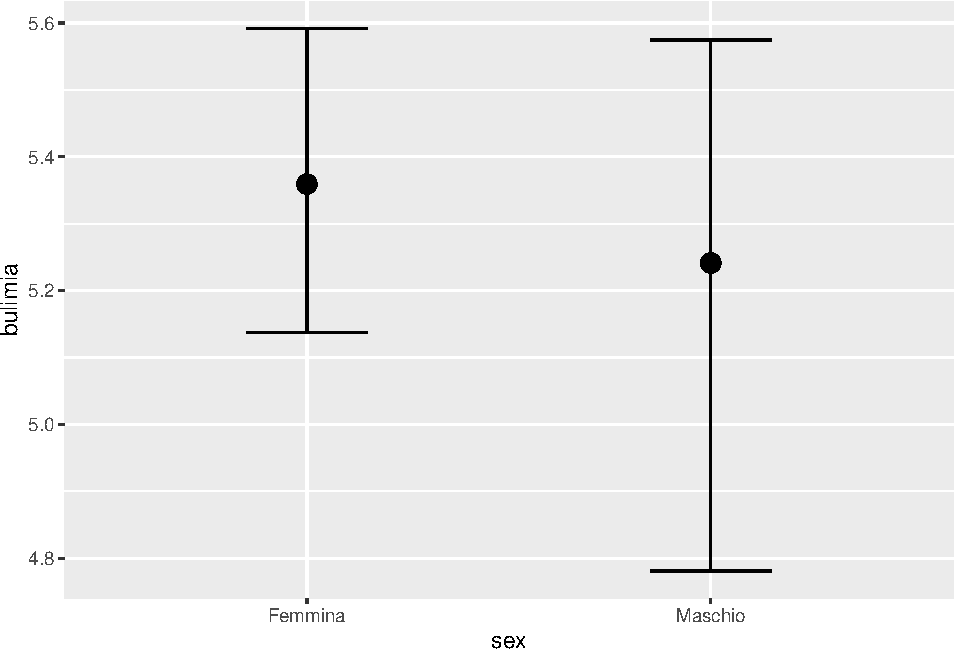
\includegraphics{050_quest_groups_files/figure-latex/unnamed-chunk-2-10.pdf}

\begin{Shaded}
\begin{Highlighting}[]
\NormalTok{m7 }\OtherTok{\textless{}{-}} \FunctionTok{brm}\NormalTok{(}
\NormalTok{  dieting }\SpecialCharTok{\textasciitilde{}}\NormalTok{ sex,}
  \AttributeTok{data =}\NormalTok{ dat, }
  \CommentTok{\# prior = prior\_ma,}
  \AttributeTok{family =} \FunctionTok{skew\_normal}\NormalTok{(),}
  \AttributeTok{control =} \FunctionTok{list}\NormalTok{(}\AttributeTok{adapt\_delta =} \FloatTok{0.98}\NormalTok{),}
  \AttributeTok{iter =} \DecValTok{4000}\NormalTok{,}
  \AttributeTok{cores =} \DecValTok{6}\NormalTok{,}
  \AttributeTok{backend =} \StringTok{"cmdstan"}
\NormalTok{)}
\end{Highlighting}
\end{Shaded}

\begin{verbatim}
## Warning: Rows containing NAs were excluded from the model.
\end{verbatim}

\begin{verbatim}
## Start sampling
\end{verbatim}

\begin{verbatim}
## Running MCMC with 4 chains, at most 6 in parallel...
## 
## Chain 1 Iteration:    1 / 4000 [  0%]  (Warmup) 
## Chain 2 Iteration:    1 / 4000 [  0%]  (Warmup) 
## Chain 3 Iteration:    1 / 4000 [  0%]  (Warmup) 
## Chain 4 Iteration:    1 / 4000 [  0%]  (Warmup) 
## Chain 1 Iteration:  100 / 4000 [  2%]  (Warmup) 
## Chain 3 Iteration:  100 / 4000 [  2%]  (Warmup) 
## Chain 1 Iteration:  200 / 4000 [  5%]  (Warmup) 
## Chain 2 Iteration:  100 / 4000 [  2%]  (Warmup) 
## Chain 2 Iteration:  200 / 4000 [  5%]  (Warmup) 
## Chain 2 Iteration:  300 / 4000 [  7%]  (Warmup) 
## Chain 3 Iteration:  200 / 4000 [  5%]  (Warmup) 
## Chain 3 Iteration:  300 / 4000 [  7%]  (Warmup) 
## Chain 4 Iteration:  100 / 4000 [  2%]  (Warmup) 
## Chain 4 Iteration:  200 / 4000 [  5%]  (Warmup) 
## Chain 1 Iteration:  300 / 4000 [  7%]  (Warmup) 
## Chain 1 Iteration:  400 / 4000 [ 10%]  (Warmup) 
## Chain 2 Iteration:  400 / 4000 [ 10%]  (Warmup) 
## Chain 2 Iteration:  500 / 4000 [ 12%]  (Warmup) 
## Chain 3 Iteration:  400 / 4000 [ 10%]  (Warmup) 
## Chain 3 Iteration:  500 / 4000 [ 12%]  (Warmup) 
## Chain 3 Iteration:  600 / 4000 [ 15%]  (Warmup) 
## Chain 4 Iteration:  300 / 4000 [  7%]  (Warmup) 
## Chain 4 Iteration:  400 / 4000 [ 10%]  (Warmup) 
## Chain 1 Iteration:  500 / 4000 [ 12%]  (Warmup) 
## Chain 1 Iteration:  600 / 4000 [ 15%]  (Warmup) 
## Chain 1 Iteration:  700 / 4000 [ 17%]  (Warmup) 
## Chain 2 Iteration:  600 / 4000 [ 15%]  (Warmup) 
## Chain 2 Iteration:  700 / 4000 [ 17%]  (Warmup) 
## Chain 2 Iteration:  800 / 4000 [ 20%]  (Warmup) 
## Chain 3 Iteration:  700 / 4000 [ 17%]  (Warmup) 
## Chain 3 Iteration:  800 / 4000 [ 20%]  (Warmup) 
## Chain 3 Iteration:  900 / 4000 [ 22%]  (Warmup) 
## Chain 4 Iteration:  500 / 4000 [ 12%]  (Warmup) 
## Chain 4 Iteration:  600 / 4000 [ 15%]  (Warmup) 
## Chain 4 Iteration:  700 / 4000 [ 17%]  (Warmup) 
## Chain 1 Iteration:  800 / 4000 [ 20%]  (Warmup) 
## Chain 1 Iteration:  900 / 4000 [ 22%]  (Warmup) 
## Chain 1 Iteration: 1000 / 4000 [ 25%]  (Warmup) 
## Chain 2 Iteration:  900 / 4000 [ 22%]  (Warmup) 
## Chain 2 Iteration: 1000 / 4000 [ 25%]  (Warmup) 
## Chain 3 Iteration: 1000 / 4000 [ 25%]  (Warmup) 
## Chain 3 Iteration: 1100 / 4000 [ 27%]  (Warmup) 
## Chain 3 Iteration: 1200 / 4000 [ 30%]  (Warmup) 
## Chain 3 Iteration: 1300 / 4000 [ 32%]  (Warmup) 
## Chain 4 Iteration:  800 / 4000 [ 20%]  (Warmup) 
## Chain 4 Iteration:  900 / 4000 [ 22%]  (Warmup) 
## Chain 1 Iteration: 1100 / 4000 [ 27%]  (Warmup) 
## Chain 1 Iteration: 1200 / 4000 [ 30%]  (Warmup) 
## Chain 1 Iteration: 1300 / 4000 [ 32%]  (Warmup) 
## Chain 2 Iteration: 1100 / 4000 [ 27%]  (Warmup) 
## Chain 2 Iteration: 1200 / 4000 [ 30%]  (Warmup) 
## Chain 2 Iteration: 1300 / 4000 [ 32%]  (Warmup) 
## Chain 3 Iteration: 1400 / 4000 [ 35%]  (Warmup) 
## Chain 3 Iteration: 1500 / 4000 [ 37%]  (Warmup) 
## Chain 3 Iteration: 1600 / 4000 [ 40%]  (Warmup) 
## Chain 4 Iteration: 1000 / 4000 [ 25%]  (Warmup) 
## Chain 4 Iteration: 1100 / 4000 [ 27%]  (Warmup) 
## Chain 4 Iteration: 1200 / 4000 [ 30%]  (Warmup) 
## Chain 4 Iteration: 1300 / 4000 [ 32%]  (Warmup) 
## Chain 1 Iteration: 1400 / 4000 [ 35%]  (Warmup) 
## Chain 1 Iteration: 1500 / 4000 [ 37%]  (Warmup) 
## Chain 1 Iteration: 1600 / 4000 [ 40%]  (Warmup) 
## Chain 2 Iteration: 1400 / 4000 [ 35%]  (Warmup) 
## Chain 2 Iteration: 1500 / 4000 [ 37%]  (Warmup) 
## Chain 2 Iteration: 1600 / 4000 [ 40%]  (Warmup) 
## Chain 3 Iteration: 1700 / 4000 [ 42%]  (Warmup) 
## Chain 3 Iteration: 1800 / 4000 [ 45%]  (Warmup) 
## Chain 3 Iteration: 1900 / 4000 [ 47%]  (Warmup) 
## Chain 4 Iteration: 1400 / 4000 [ 35%]  (Warmup) 
## Chain 4 Iteration: 1500 / 4000 [ 37%]  (Warmup) 
## Chain 1 Iteration: 1700 / 4000 [ 42%]  (Warmup) 
## Chain 1 Iteration: 1800 / 4000 [ 45%]  (Warmup) 
## Chain 1 Iteration: 1900 / 4000 [ 47%]  (Warmup) 
## Chain 2 Iteration: 1700 / 4000 [ 42%]  (Warmup) 
## Chain 2 Iteration: 1800 / 4000 [ 45%]  (Warmup) 
## Chain 2 Iteration: 1900 / 4000 [ 47%]  (Warmup) 
## Chain 3 Iteration: 2000 / 4000 [ 50%]  (Warmup) 
## Chain 3 Iteration: 2001 / 4000 [ 50%]  (Sampling) 
## Chain 4 Iteration: 1600 / 4000 [ 40%]  (Warmup) 
## Chain 4 Iteration: 1700 / 4000 [ 42%]  (Warmup) 
## Chain 4 Iteration: 1800 / 4000 [ 45%]  (Warmup) 
## Chain 1 Iteration: 2000 / 4000 [ 50%]  (Warmup) 
## Chain 1 Iteration: 2001 / 4000 [ 50%]  (Sampling) 
## Chain 2 Iteration: 2000 / 4000 [ 50%]  (Warmup) 
## Chain 2 Iteration: 2001 / 4000 [ 50%]  (Sampling) 
## Chain 2 Iteration: 2100 / 4000 [ 52%]  (Sampling) 
## Chain 3 Iteration: 2100 / 4000 [ 52%]  (Sampling) 
## Chain 3 Iteration: 2200 / 4000 [ 55%]  (Sampling) 
## Chain 4 Iteration: 1900 / 4000 [ 47%]  (Warmup) 
## Chain 4 Iteration: 2000 / 4000 [ 50%]  (Warmup) 
## Chain 4 Iteration: 2001 / 4000 [ 50%]  (Sampling) 
## Chain 1 Iteration: 2100 / 4000 [ 52%]  (Sampling) 
## Chain 1 Iteration: 2200 / 4000 [ 55%]  (Sampling) 
## Chain 2 Iteration: 2200 / 4000 [ 55%]  (Sampling) 
## Chain 3 Iteration: 2300 / 4000 [ 57%]  (Sampling) 
## Chain 4 Iteration: 2100 / 4000 [ 52%]  (Sampling) 
## Chain 1 Iteration: 2300 / 4000 [ 57%]  (Sampling) 
## Chain 1 Iteration: 2400 / 4000 [ 60%]  (Sampling) 
## Chain 2 Iteration: 2300 / 4000 [ 57%]  (Sampling) 
## Chain 2 Iteration: 2400 / 4000 [ 60%]  (Sampling) 
## Chain 3 Iteration: 2400 / 4000 [ 60%]  (Sampling) 
## Chain 4 Iteration: 2200 / 4000 [ 55%]  (Sampling) 
## Chain 4 Iteration: 2300 / 4000 [ 57%]  (Sampling) 
## Chain 1 Iteration: 2500 / 4000 [ 62%]  (Sampling) 
## Chain 1 Iteration: 2600 / 4000 [ 65%]  (Sampling) 
## Chain 2 Iteration: 2500 / 4000 [ 62%]  (Sampling) 
## Chain 2 Iteration: 2600 / 4000 [ 65%]  (Sampling) 
## Chain 3 Iteration: 2500 / 4000 [ 62%]  (Sampling) 
## Chain 3 Iteration: 2600 / 4000 [ 65%]  (Sampling) 
## Chain 4 Iteration: 2400 / 4000 [ 60%]  (Sampling) 
## Chain 4 Iteration: 2500 / 4000 [ 62%]  (Sampling) 
## Chain 1 Iteration: 2700 / 4000 [ 67%]  (Sampling) 
## Chain 1 Iteration: 2800 / 4000 [ 70%]  (Sampling) 
## Chain 2 Iteration: 2700 / 4000 [ 67%]  (Sampling) 
## Chain 2 Iteration: 2800 / 4000 [ 70%]  (Sampling) 
## Chain 3 Iteration: 2700 / 4000 [ 67%]  (Sampling) 
## Chain 3 Iteration: 2800 / 4000 [ 70%]  (Sampling) 
## Chain 4 Iteration: 2600 / 4000 [ 65%]  (Sampling) 
## Chain 4 Iteration: 2700 / 4000 [ 67%]  (Sampling) 
## Chain 1 Iteration: 2900 / 4000 [ 72%]  (Sampling) 
## Chain 1 Iteration: 3000 / 4000 [ 75%]  (Sampling) 
## Chain 2 Iteration: 2900 / 4000 [ 72%]  (Sampling) 
## Chain 2 Iteration: 3000 / 4000 [ 75%]  (Sampling) 
## Chain 3 Iteration: 2900 / 4000 [ 72%]  (Sampling) 
## Chain 3 Iteration: 3000 / 4000 [ 75%]  (Sampling) 
## Chain 4 Iteration: 2800 / 4000 [ 70%]  (Sampling) 
## Chain 4 Iteration: 2900 / 4000 [ 72%]  (Sampling) 
## Chain 4 Iteration: 3000 / 4000 [ 75%]  (Sampling) 
## Chain 1 Iteration: 3100 / 4000 [ 77%]  (Sampling) 
## Chain 1 Iteration: 3200 / 4000 [ 80%]  (Sampling) 
## Chain 1 Iteration: 3300 / 4000 [ 82%]  (Sampling) 
## Chain 2 Iteration: 3100 / 4000 [ 77%]  (Sampling) 
## Chain 2 Iteration: 3200 / 4000 [ 80%]  (Sampling) 
## Chain 2 Iteration: 3300 / 4000 [ 82%]  (Sampling) 
## Chain 3 Iteration: 3100 / 4000 [ 77%]  (Sampling) 
## Chain 3 Iteration: 3200 / 4000 [ 80%]  (Sampling) 
## Chain 4 Iteration: 3100 / 4000 [ 77%]  (Sampling) 
## Chain 4 Iteration: 3200 / 4000 [ 80%]  (Sampling) 
## Chain 1 Iteration: 3400 / 4000 [ 85%]  (Sampling) 
## Chain 1 Iteration: 3500 / 4000 [ 87%]  (Sampling) 
## Chain 2 Iteration: 3400 / 4000 [ 85%]  (Sampling) 
## Chain 2 Iteration: 3500 / 4000 [ 87%]  (Sampling) 
## Chain 3 Iteration: 3300 / 4000 [ 82%]  (Sampling) 
## Chain 3 Iteration: 3400 / 4000 [ 85%]  (Sampling) 
## Chain 4 Iteration: 3300 / 4000 [ 82%]  (Sampling) 
## Chain 4 Iteration: 3400 / 4000 [ 85%]  (Sampling) 
## Chain 1 Iteration: 3600 / 4000 [ 90%]  (Sampling) 
## Chain 1 Iteration: 3700 / 4000 [ 92%]  (Sampling) 
## Chain 2 Iteration: 3600 / 4000 [ 90%]  (Sampling) 
## Chain 2 Iteration: 3700 / 4000 [ 92%]  (Sampling) 
## Chain 3 Iteration: 3500 / 4000 [ 87%]  (Sampling) 
## Chain 3 Iteration: 3600 / 4000 [ 90%]  (Sampling) 
## Chain 4 Iteration: 3500 / 4000 [ 87%]  (Sampling) 
## Chain 4 Iteration: 3600 / 4000 [ 90%]  (Sampling) 
## Chain 1 Iteration: 3800 / 4000 [ 95%]  (Sampling) 
## Chain 2 Iteration: 3800 / 4000 [ 95%]  (Sampling) 
## Chain 3 Iteration: 3700 / 4000 [ 92%]  (Sampling) 
## Chain 4 Iteration: 3700 / 4000 [ 92%]  (Sampling) 
## Chain 1 Iteration: 3900 / 4000 [ 97%]  (Sampling) 
## Chain 1 Iteration: 4000 / 4000 [100%]  (Sampling) 
## Chain 2 Iteration: 3900 / 4000 [ 97%]  (Sampling) 
## Chain 2 Iteration: 4000 / 4000 [100%]  (Sampling) 
## Chain 3 Iteration: 3800 / 4000 [ 95%]  (Sampling) 
## Chain 4 Iteration: 3800 / 4000 [ 95%]  (Sampling) 
## Chain 4 Iteration: 3900 / 4000 [ 97%]  (Sampling) 
## Chain 1 finished in 2.1 seconds.
## Chain 2 finished in 2.1 seconds.
## Chain 3 Iteration: 3900 / 4000 [ 97%]  (Sampling) 
## Chain 4 Iteration: 4000 / 4000 [100%]  (Sampling) 
## Chain 4 finished in 2.2 seconds.
## Chain 3 Iteration: 4000 / 4000 [100%]  (Sampling) 
## Chain 3 finished in 2.2 seconds.
## 
## All 4 chains finished successfully.
## Mean chain execution time: 2.1 seconds.
## Total execution time: 2.5 seconds.
\end{verbatim}

\begin{Shaded}
\begin{Highlighting}[]
\FunctionTok{summary}\NormalTok{(m7)}
\end{Highlighting}
\end{Shaded}

\begin{verbatim}
##  Family: skew_normal 
##   Links: mu = identity; sigma = identity; alpha = identity 
## Formula: dieting ~ sex 
##    Data: dat (Number of observations: 266) 
## Samples: 4 chains, each with iter = 4000; warmup = 2000; thin = 1;
##          total post-warmup samples = 8000
## 
## Population-Level Effects: 
##            Estimate Est.Error l-95% CI u-95% CI Rhat Bulk_ESS Tail_ESS
## Intercept      7.32      0.35     6.67     8.04 1.00     3226     3521
## sexMaschio    -0.84      0.55    -2.07     0.08 1.00     5028     3454
## 
## Family Specific Parameters: 
##       Estimate Est.Error l-95% CI u-95% CI Rhat Bulk_ESS Tail_ESS
## sigma     5.87      0.26     5.40     6.40 1.00     3178     3786
## alpha    13.37      2.29     9.32    18.29 1.00     4127     3557
## 
## Samples were drawn using sample(hmc). For each parameter, Bulk_ESS
## and Tail_ESS are effective sample size measures, and Rhat is the potential
## scale reduction factor on split chains (at convergence, Rhat = 1).
\end{verbatim}

\begin{Shaded}
\begin{Highlighting}[]
\FunctionTok{plot}\NormalTok{(}\FunctionTok{conditional\_effects}\NormalTok{(m7, }\StringTok{"sex"}\NormalTok{))}
\end{Highlighting}
\end{Shaded}

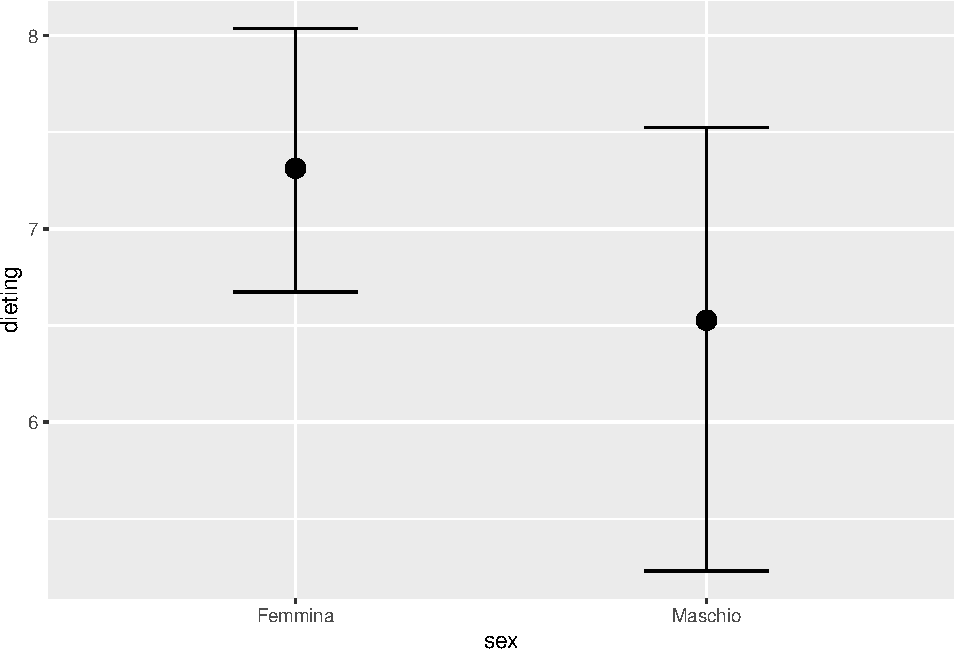
\includegraphics{050_quest_groups_files/figure-latex/unnamed-chunk-2-11.pdf}

\begin{Shaded}
\begin{Highlighting}[]
\NormalTok{dat }\SpecialCharTok{\%\textgreater{}\%} 
  \FunctionTok{group\_by}\NormalTok{(sex) }\SpecialCharTok{\%\textgreater{}\%} 
  \FunctionTok{summarise}\NormalTok{(}
    \AttributeTok{avg\_bsq14 =} \FunctionTok{mean}\NormalTok{(bsq14\_tot, }\AttributeTok{trim =} \FloatTok{0.1}\NormalTok{, }\AttributeTok{na.rm =} \ConstantTok{TRUE}\NormalTok{)}
\NormalTok{  )}
\end{Highlighting}
\end{Shaded}

\begin{verbatim}
## # A tibble: 2 x 2
##   sex     avg_bsq14
##   <chr>       <dbl>
## 1 Femmina      43.1
## 2 Maschio      30.0
\end{verbatim}

\begin{Shaded}
\begin{Highlighting}[]
\CommentTok{\# Prevalence of body image dissatisfaction among youth in the United Arab }
\CommentTok{\# Emirates: gender, age, and body mass index differences}
\CommentTok{\# Siham Alharballeh1 \& Hamzeh Dodeen}
\FunctionTok{hist}\NormalTok{(dat}\SpecialCharTok{$}\NormalTok{bsq14)}
\end{Highlighting}
\end{Shaded}

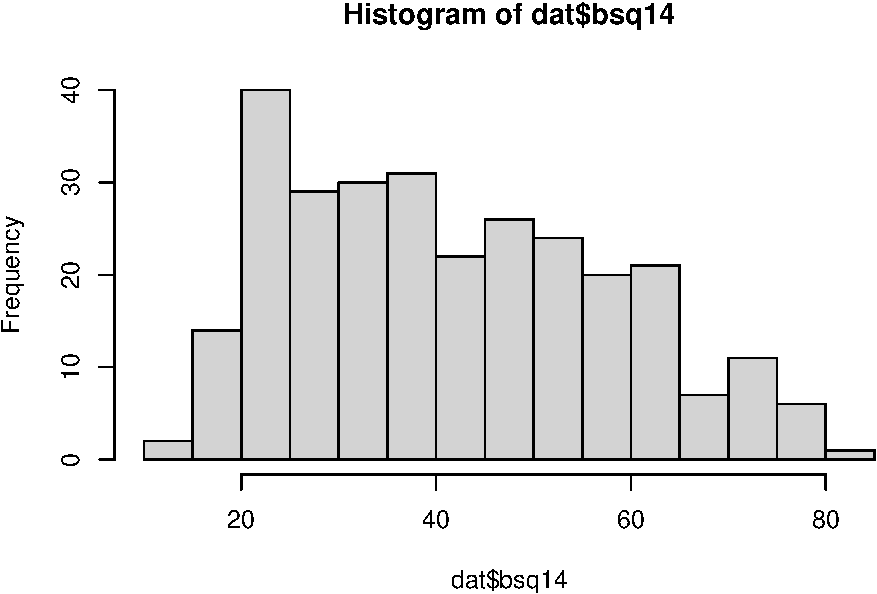
\includegraphics{050_quest_groups_files/figure-latex/unnamed-chunk-2-12.pdf}

\begin{Shaded}
\begin{Highlighting}[]
\NormalTok{fm0 }\OtherTok{\textless{}{-}} \FunctionTok{brm}\NormalTok{(}
\NormalTok{  bsq14\_tot }\SpecialCharTok{\textasciitilde{}}\NormalTok{ age }\SpecialCharTok{+}\NormalTok{ bmi }\SpecialCharTok{+}\NormalTok{ sex,}
  \AttributeTok{data =}\NormalTok{ dat, }
  \CommentTok{\# prior = prior\_ma,}
  \AttributeTok{family =} \FunctionTok{skew\_normal}\NormalTok{(),}
  \AttributeTok{control =} \FunctionTok{list}\NormalTok{(}\AttributeTok{adapt\_delta =} \FloatTok{0.98}\NormalTok{),}
  \AttributeTok{iter =} \DecValTok{4000}\NormalTok{,}
  \AttributeTok{cores =} \DecValTok{6}\NormalTok{,}
  \AttributeTok{backend =} \StringTok{"cmdstan"}
\NormalTok{)}
\end{Highlighting}
\end{Shaded}

\begin{verbatim}
## Warning: Rows containing NAs were excluded from the model.
\end{verbatim}

\begin{verbatim}
## Start sampling
\end{verbatim}

\begin{verbatim}
## Running MCMC with 4 chains, at most 6 in parallel...
## 
## Chain 1 Iteration:    1 / 4000 [  0%]  (Warmup) 
## Chain 2 Iteration:    1 / 4000 [  0%]  (Warmup) 
## Chain 3 Iteration:    1 / 4000 [  0%]  (Warmup)
\end{verbatim}

\begin{verbatim}
## Chain 4 Rejecting initial value:
\end{verbatim}

\begin{verbatim}
## Chain 4   Log probability evaluates to log(0), i.e. negative infinity.
\end{verbatim}

\begin{verbatim}
## Chain 4   Stan can't start sampling from this initial value.
\end{verbatim}

\begin{verbatim}
## Chain 4 Iteration:    1 / 4000 [  0%]  (Warmup) 
## Chain 2 Iteration:  100 / 4000 [  2%]  (Warmup) 
## Chain 4 Iteration:  100 / 4000 [  2%]  (Warmup) 
## Chain 2 Iteration:  200 / 4000 [  5%]  (Warmup) 
## Chain 2 Iteration:  300 / 4000 [  7%]  (Warmup) 
## Chain 3 Iteration:  100 / 4000 [  2%]  (Warmup) 
## Chain 4 Iteration:  200 / 4000 [  5%]  (Warmup) 
## Chain 4 Iteration:  300 / 4000 [  7%]  (Warmup) 
## Chain 2 Iteration:  400 / 4000 [ 10%]  (Warmup) 
## Chain 2 Iteration:  500 / 4000 [ 12%]  (Warmup) 
## Chain 2 Iteration:  600 / 4000 [ 15%]  (Warmup) 
## Chain 3 Iteration:  200 / 4000 [  5%]  (Warmup) 
## Chain 3 Iteration:  300 / 4000 [  7%]  (Warmup) 
## Chain 3 Iteration:  400 / 4000 [ 10%]  (Warmup) 
## Chain 4 Iteration:  400 / 4000 [ 10%]  (Warmup) 
## Chain 4 Iteration:  500 / 4000 [ 12%]  (Warmup) 
## Chain 1 Iteration:  100 / 4000 [  2%]  (Warmup) 
## Chain 2 Iteration:  700 / 4000 [ 17%]  (Warmup) 
## Chain 2 Iteration:  800 / 4000 [ 20%]  (Warmup) 
## Chain 3 Iteration:  500 / 4000 [ 12%]  (Warmup) 
## Chain 3 Iteration:  600 / 4000 [ 15%]  (Warmup) 
## Chain 3 Iteration:  700 / 4000 [ 17%]  (Warmup) 
## Chain 4 Iteration:  600 / 4000 [ 15%]  (Warmup) 
## Chain 4 Iteration:  700 / 4000 [ 17%]  (Warmup) 
## Chain 4 Iteration:  800 / 4000 [ 20%]  (Warmup) 
## Chain 1 Iteration:  200 / 4000 [  5%]  (Warmup) 
## Chain 1 Iteration:  300 / 4000 [  7%]  (Warmup) 
## Chain 2 Iteration:  900 / 4000 [ 22%]  (Warmup) 
## Chain 2 Iteration: 1000 / 4000 [ 25%]  (Warmup) 
## Chain 2 Iteration: 1100 / 4000 [ 27%]  (Warmup) 
## Chain 3 Iteration:  800 / 4000 [ 20%]  (Warmup) 
## Chain 3 Iteration:  900 / 4000 [ 22%]  (Warmup) 
## Chain 4 Iteration:  900 / 4000 [ 22%]  (Warmup) 
## Chain 4 Iteration: 1000 / 4000 [ 25%]  (Warmup) 
## Chain 4 Iteration: 1100 / 4000 [ 27%]  (Warmup) 
## Chain 1 Iteration:  400 / 4000 [ 10%]  (Warmup) 
## Chain 1 Iteration:  500 / 4000 [ 12%]  (Warmup) 
## Chain 1 Iteration:  600 / 4000 [ 15%]  (Warmup) 
## Chain 2 Iteration: 1200 / 4000 [ 30%]  (Warmup) 
## Chain 2 Iteration: 1300 / 4000 [ 32%]  (Warmup) 
## Chain 2 Iteration: 1400 / 4000 [ 35%]  (Warmup) 
## Chain 3 Iteration: 1000 / 4000 [ 25%]  (Warmup) 
## Chain 3 Iteration: 1100 / 4000 [ 27%]  (Warmup) 
## Chain 3 Iteration: 1200 / 4000 [ 30%]  (Warmup) 
## Chain 4 Iteration: 1200 / 4000 [ 30%]  (Warmup) 
## Chain 4 Iteration: 1300 / 4000 [ 32%]  (Warmup) 
## Chain 4 Iteration: 1400 / 4000 [ 35%]  (Warmup) 
## Chain 1 Iteration:  700 / 4000 [ 17%]  (Warmup) 
## Chain 1 Iteration:  800 / 4000 [ 20%]  (Warmup) 
## Chain 2 Iteration: 1500 / 4000 [ 37%]  (Warmup) 
## Chain 2 Iteration: 1600 / 4000 [ 40%]  (Warmup) 
## Chain 2 Iteration: 1700 / 4000 [ 42%]  (Warmup) 
## Chain 3 Iteration: 1300 / 4000 [ 32%]  (Warmup) 
## Chain 3 Iteration: 1400 / 4000 [ 35%]  (Warmup) 
## Chain 3 Iteration: 1500 / 4000 [ 37%]  (Warmup) 
## Chain 4 Iteration: 1500 / 4000 [ 37%]  (Warmup) 
## Chain 4 Iteration: 1600 / 4000 [ 40%]  (Warmup) 
## Chain 4 Iteration: 1700 / 4000 [ 42%]  (Warmup) 
## Chain 1 Iteration:  900 / 4000 [ 22%]  (Warmup) 
## Chain 1 Iteration: 1000 / 4000 [ 25%]  (Warmup) 
## Chain 1 Iteration: 1100 / 4000 [ 27%]  (Warmup) 
## Chain 1 Iteration: 1200 / 4000 [ 30%]  (Warmup) 
## Chain 2 Iteration: 1800 / 4000 [ 45%]  (Warmup) 
## Chain 2 Iteration: 1900 / 4000 [ 47%]  (Warmup) 
## Chain 2 Iteration: 2000 / 4000 [ 50%]  (Warmup) 
## Chain 2 Iteration: 2001 / 4000 [ 50%]  (Sampling) 
## Chain 3 Iteration: 1600 / 4000 [ 40%]  (Warmup) 
## Chain 3 Iteration: 1700 / 4000 [ 42%]  (Warmup) 
## Chain 3 Iteration: 1800 / 4000 [ 45%]  (Warmup) 
## Chain 4 Iteration: 1800 / 4000 [ 45%]  (Warmup) 
## Chain 4 Iteration: 1900 / 4000 [ 47%]  (Warmup) 
## Chain 4 Iteration: 2000 / 4000 [ 50%]  (Warmup) 
## Chain 4 Iteration: 2001 / 4000 [ 50%]  (Sampling) 
## Chain 1 Iteration: 1300 / 4000 [ 32%]  (Warmup) 
## Chain 1 Iteration: 1400 / 4000 [ 35%]  (Warmup) 
## Chain 1 Iteration: 1500 / 4000 [ 37%]  (Warmup) 
## Chain 2 Iteration: 2100 / 4000 [ 52%]  (Sampling) 
## Chain 2 Iteration: 2200 / 4000 [ 55%]  (Sampling) 
## Chain 2 Iteration: 2300 / 4000 [ 57%]  (Sampling) 
## Chain 3 Iteration: 1900 / 4000 [ 47%]  (Warmup) 
## Chain 3 Iteration: 2000 / 4000 [ 50%]  (Warmup) 
## Chain 3 Iteration: 2001 / 4000 [ 50%]  (Sampling) 
## Chain 4 Iteration: 2100 / 4000 [ 52%]  (Sampling) 
## Chain 4 Iteration: 2200 / 4000 [ 55%]  (Sampling) 
## Chain 1 Iteration: 1600 / 4000 [ 40%]  (Warmup) 
## Chain 1 Iteration: 1700 / 4000 [ 42%]  (Warmup) 
## Chain 2 Iteration: 2400 / 4000 [ 60%]  (Sampling) 
## Chain 2 Iteration: 2500 / 4000 [ 62%]  (Sampling) 
## Chain 2 Iteration: 2600 / 4000 [ 65%]  (Sampling) 
## Chain 3 Iteration: 2100 / 4000 [ 52%]  (Sampling) 
## Chain 3 Iteration: 2200 / 4000 [ 55%]  (Sampling) 
## Chain 4 Iteration: 2300 / 4000 [ 57%]  (Sampling) 
## Chain 4 Iteration: 2400 / 4000 [ 60%]  (Sampling) 
## Chain 4 Iteration: 2500 / 4000 [ 62%]  (Sampling) 
## Chain 1 Iteration: 1800 / 4000 [ 45%]  (Warmup) 
## Chain 1 Iteration: 1900 / 4000 [ 47%]  (Warmup) 
## Chain 1 Iteration: 2000 / 4000 [ 50%]  (Warmup) 
## Chain 1 Iteration: 2001 / 4000 [ 50%]  (Sampling) 
## Chain 2 Iteration: 2700 / 4000 [ 67%]  (Sampling) 
## Chain 2 Iteration: 2800 / 4000 [ 70%]  (Sampling) 
## Chain 3 Iteration: 2300 / 4000 [ 57%]  (Sampling) 
## Chain 3 Iteration: 2400 / 4000 [ 60%]  (Sampling) 
## Chain 3 Iteration: 2500 / 4000 [ 62%]  (Sampling) 
## Chain 4 Iteration: 2600 / 4000 [ 65%]  (Sampling) 
## Chain 4 Iteration: 2700 / 4000 [ 67%]  (Sampling) 
## Chain 1 Iteration: 2100 / 4000 [ 52%]  (Sampling) 
## Chain 1 Iteration: 2200 / 4000 [ 55%]  (Sampling) 
## Chain 2 Iteration: 2900 / 4000 [ 72%]  (Sampling) 
## Chain 2 Iteration: 3000 / 4000 [ 75%]  (Sampling) 
## Chain 2 Iteration: 3100 / 4000 [ 77%]  (Sampling) 
## Chain 3 Iteration: 2600 / 4000 [ 65%]  (Sampling) 
## Chain 3 Iteration: 2700 / 4000 [ 67%]  (Sampling) 
## Chain 4 Iteration: 2800 / 4000 [ 70%]  (Sampling) 
## Chain 4 Iteration: 2900 / 4000 [ 72%]  (Sampling) 
## Chain 1 Iteration: 2300 / 4000 [ 57%]  (Sampling) 
## Chain 1 Iteration: 2400 / 4000 [ 60%]  (Sampling) 
## Chain 2 Iteration: 3200 / 4000 [ 80%]  (Sampling) 
## Chain 2 Iteration: 3300 / 4000 [ 82%]  (Sampling) 
## Chain 2 Iteration: 3400 / 4000 [ 85%]  (Sampling) 
## Chain 3 Iteration: 2800 / 4000 [ 70%]  (Sampling) 
## Chain 3 Iteration: 2900 / 4000 [ 72%]  (Sampling) 
## Chain 4 Iteration: 3000 / 4000 [ 75%]  (Sampling) 
## Chain 4 Iteration: 3100 / 4000 [ 77%]  (Sampling) 
## Chain 4 Iteration: 3200 / 4000 [ 80%]  (Sampling) 
## Chain 1 Iteration: 2500 / 4000 [ 62%]  (Sampling) 
## Chain 1 Iteration: 2600 / 4000 [ 65%]  (Sampling) 
## Chain 2 Iteration: 3500 / 4000 [ 87%]  (Sampling) 
## Chain 2 Iteration: 3600 / 4000 [ 90%]  (Sampling) 
## Chain 3 Iteration: 3000 / 4000 [ 75%]  (Sampling) 
## Chain 3 Iteration: 3100 / 4000 [ 77%]  (Sampling) 
## Chain 3 Iteration: 3200 / 4000 [ 80%]  (Sampling) 
## Chain 4 Iteration: 3300 / 4000 [ 82%]  (Sampling) 
## Chain 4 Iteration: 3400 / 4000 [ 85%]  (Sampling) 
## Chain 1 Iteration: 2700 / 4000 [ 67%]  (Sampling) 
## Chain 1 Iteration: 2800 / 4000 [ 70%]  (Sampling) 
## Chain 2 Iteration: 3700 / 4000 [ 92%]  (Sampling) 
## Chain 2 Iteration: 3800 / 4000 [ 95%]  (Sampling) 
## Chain 2 Iteration: 3900 / 4000 [ 97%]  (Sampling) 
## Chain 3 Iteration: 3300 / 4000 [ 82%]  (Sampling) 
## Chain 3 Iteration: 3400 / 4000 [ 85%]  (Sampling) 
## Chain 4 Iteration: 3500 / 4000 [ 87%]  (Sampling) 
## Chain 4 Iteration: 3600 / 4000 [ 90%]  (Sampling) 
## Chain 1 Iteration: 2900 / 4000 [ 72%]  (Sampling) 
## Chain 1 Iteration: 3000 / 4000 [ 75%]  (Sampling) 
## Chain 2 Iteration: 4000 / 4000 [100%]  (Sampling) 
## Chain 3 Iteration: 3500 / 4000 [ 87%]  (Sampling) 
## Chain 3 Iteration: 3600 / 4000 [ 90%]  (Sampling) 
## Chain 4 Iteration: 3700 / 4000 [ 92%]  (Sampling) 
## Chain 4 Iteration: 3800 / 4000 [ 95%]  (Sampling) 
## Chain 4 Iteration: 3900 / 4000 [ 97%]  (Sampling) 
## Chain 2 finished in 1.7 seconds.
## Chain 1 Iteration: 3100 / 4000 [ 77%]  (Sampling) 
## Chain 1 Iteration: 3200 / 4000 [ 80%]  (Sampling) 
## Chain 3 Iteration: 3700 / 4000 [ 92%]  (Sampling) 
## Chain 3 Iteration: 3800 / 4000 [ 95%]  (Sampling) 
## Chain 3 Iteration: 3900 / 4000 [ 97%]  (Sampling) 
## Chain 4 Iteration: 4000 / 4000 [100%]  (Sampling) 
## Chain 4 finished in 1.8 seconds.
## Chain 1 Iteration: 3300 / 4000 [ 82%]  (Sampling) 
## Chain 1 Iteration: 3400 / 4000 [ 85%]  (Sampling) 
## Chain 3 Iteration: 4000 / 4000 [100%]  (Sampling) 
## Chain 3 finished in 1.9 seconds.
## Chain 1 Iteration: 3500 / 4000 [ 87%]  (Sampling) 
## Chain 1 Iteration: 3600 / 4000 [ 90%]  (Sampling) 
## Chain 1 Iteration: 3700 / 4000 [ 92%]  (Sampling) 
## Chain 1 Iteration: 3800 / 4000 [ 95%]  (Sampling) 
## Chain 1 Iteration: 3900 / 4000 [ 97%]  (Sampling) 
## Chain 1 Iteration: 4000 / 4000 [100%]  (Sampling) 
## Chain 1 finished in 2.3 seconds.
## 
## All 4 chains finished successfully.
## Mean chain execution time: 1.9 seconds.
## Total execution time: 2.5 seconds.
\end{verbatim}

\begin{Shaded}
\begin{Highlighting}[]
\FunctionTok{summary}\NormalTok{(fm0)}
\end{Highlighting}
\end{Shaded}

\begin{verbatim}
##  Family: skew_normal 
##   Links: mu = identity; sigma = identity; alpha = identity 
## Formula: bsq14_tot ~ age + bmi + sex 
##    Data: dat (Number of observations: 283) 
## Samples: 4 chains, each with iter = 4000; warmup = 2000; thin = 1;
##          total post-warmup samples = 8000
## 
## Population-Level Effects: 
##            Estimate Est.Error l-95% CI u-95% CI Rhat Bulk_ESS Tail_ESS
## Intercept     20.66      4.70    11.84    30.42 1.00     8315     5528
## age           -0.03      0.18    -0.41     0.30 1.00     6618     5171
## bmi            1.06      0.15     0.74     1.34 1.00     6798     5099
## sexMaschio    -8.54      1.87   -12.43    -5.05 1.00     6441     5390
## 
## Family Specific Parameters: 
##       Estimate Est.Error l-95% CI u-95% CI Rhat Bulk_ESS Tail_ESS
## sigma    15.99      0.74    14.59    17.50 1.00     4888     5428
## alpha     7.43      1.79     4.37    11.41 1.00     5025     4541
## 
## Samples were drawn using sample(hmc). For each parameter, Bulk_ESS
## and Tail_ESS are effective sample size measures, and Rhat is the potential
## scale reduction factor on split chains (at convergence, Rhat = 1).
\end{verbatim}

\begin{Shaded}
\begin{Highlighting}[]
\FunctionTok{plot}\NormalTok{(}\FunctionTok{conditional\_effects}\NormalTok{(fm0, }\StringTok{"bmi"}\NormalTok{))}
\end{Highlighting}
\end{Shaded}

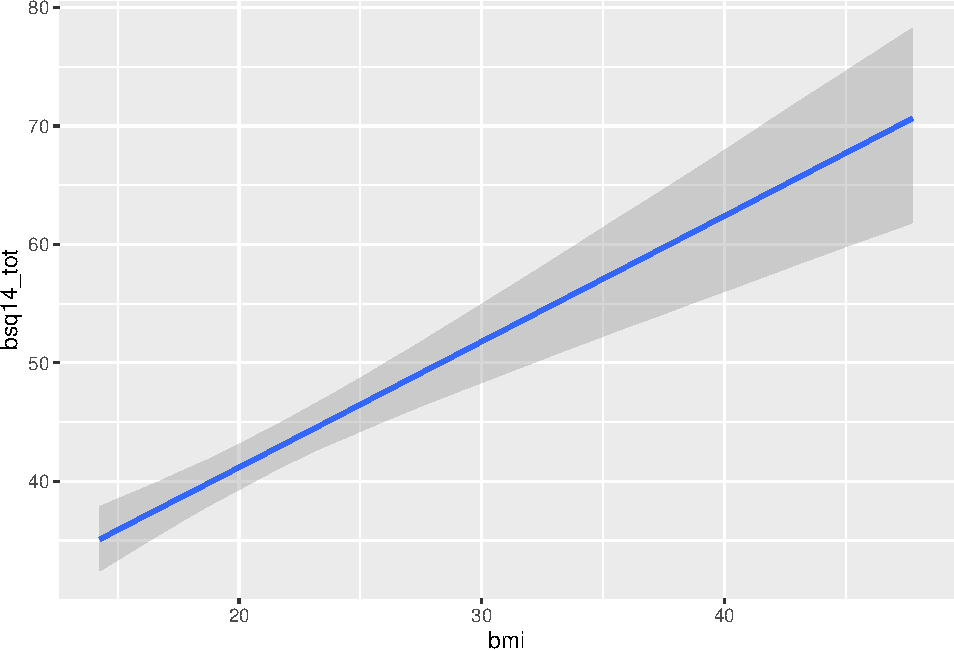
\includegraphics{050_quest_groups_files/figure-latex/unnamed-chunk-2-13.pdf}

\begin{Shaded}
\begin{Highlighting}[]
\FunctionTok{plot}\NormalTok{(}\FunctionTok{conditional\_effects}\NormalTok{(fm0, }\StringTok{"sex"}\NormalTok{))}
\end{Highlighting}
\end{Shaded}

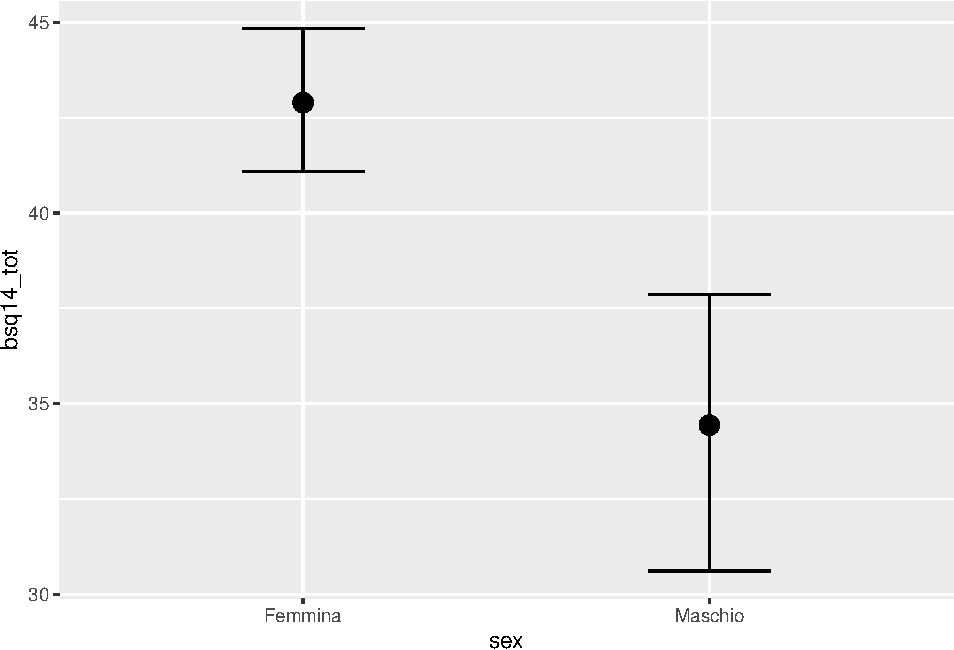
\includegraphics{050_quest_groups_files/figure-latex/unnamed-chunk-2-14.pdf}

\begin{Shaded}
\begin{Highlighting}[]
\CommentTok{\# plot(conditional\_effects(fm1, "is\_patient:sex"))}

\NormalTok{fm1 }\OtherTok{\textless{}{-}} \FunctionTok{brm}\NormalTok{(}
\NormalTok{  eat26\_tot }\SpecialCharTok{\textasciitilde{}}\NormalTok{ bsq14\_tot }\SpecialCharTok{*}\NormalTok{ (sex }\SpecialCharTok{+}\NormalTok{ is\_patient) }\SpecialCharTok{+}\NormalTok{ age }\SpecialCharTok{+}\NormalTok{ bmi,}
  \AttributeTok{data =}\NormalTok{ dat, }
  \CommentTok{\# prior = prior\_ma,}
  \AttributeTok{family =} \FunctionTok{skew\_normal}\NormalTok{(),}
  \AttributeTok{control =} \FunctionTok{list}\NormalTok{(}\AttributeTok{adapt\_delta =} \FloatTok{0.98}\NormalTok{),}
  \AttributeTok{iter =} \DecValTok{4000}\NormalTok{,}
  \AttributeTok{cores =} \DecValTok{6}\NormalTok{,}
  \AttributeTok{backend =} \StringTok{"cmdstan"}
\NormalTok{)}
\end{Highlighting}
\end{Shaded}

\begin{verbatim}
## Warning: Rows containing NAs were excluded from the model.
\end{verbatim}

\begin{verbatim}
## Start sampling
\end{verbatim}

\begin{verbatim}
## Running MCMC with 4 chains, at most 6 in parallel...
## 
## Chain 1 Iteration:    1 / 4000 [  0%]  (Warmup)
\end{verbatim}

\begin{verbatim}
## Chain 2 Rejecting initial value:
\end{verbatim}

\begin{verbatim}
## Chain 2   Log probability evaluates to log(0), i.e. negative infinity.
\end{verbatim}

\begin{verbatim}
## Chain 2   Stan can't start sampling from this initial value.
\end{verbatim}

\begin{verbatim}
## Chain 2 Rejecting initial value:
\end{verbatim}

\begin{verbatim}
## Chain 2   Log probability evaluates to log(0), i.e. negative infinity.
\end{verbatim}

\begin{verbatim}
## Chain 2   Stan can't start sampling from this initial value.
\end{verbatim}

\begin{verbatim}
## Chain 2 Rejecting initial value:
\end{verbatim}

\begin{verbatim}
## Chain 2   Log probability evaluates to log(0), i.e. negative infinity.
\end{verbatim}

\begin{verbatim}
## Chain 2   Stan can't start sampling from this initial value.
\end{verbatim}

\begin{verbatim}
## Chain 2 Rejecting initial value:
\end{verbatim}

\begin{verbatim}
## Chain 2   Log probability evaluates to log(0), i.e. negative infinity.
\end{verbatim}

\begin{verbatim}
## Chain 2   Stan can't start sampling from this initial value.
\end{verbatim}

\begin{verbatim}
## Chain 2 Rejecting initial value:
\end{verbatim}

\begin{verbatim}
## Chain 2   Log probability evaluates to log(0), i.e. negative infinity.
\end{verbatim}

\begin{verbatim}
## Chain 2   Stan can't start sampling from this initial value.
\end{verbatim}

\begin{verbatim}
## Chain 2 Rejecting initial value:
\end{verbatim}

\begin{verbatim}
## Chain 2   Log probability evaluates to log(0), i.e. negative infinity.
\end{verbatim}

\begin{verbatim}
## Chain 2   Stan can't start sampling from this initial value.
\end{verbatim}

\begin{verbatim}
## Chain 2 Rejecting initial value:
\end{verbatim}

\begin{verbatim}
## Chain 2   Log probability evaluates to log(0), i.e. negative infinity.
\end{verbatim}

\begin{verbatim}
## Chain 2   Stan can't start sampling from this initial value.
\end{verbatim}

\begin{verbatim}
## Chain 2 Rejecting initial value:
\end{verbatim}

\begin{verbatim}
## Chain 2   Log probability evaluates to log(0), i.e. negative infinity.
\end{verbatim}

\begin{verbatim}
## Chain 2   Stan can't start sampling from this initial value.
\end{verbatim}

\begin{verbatim}
## Chain 2 Rejecting initial value:
\end{verbatim}

\begin{verbatim}
## Chain 2   Log probability evaluates to log(0), i.e. negative infinity.
\end{verbatim}

\begin{verbatim}
## Chain 2   Stan can't start sampling from this initial value.
\end{verbatim}

\begin{verbatim}
## Chain 2 Rejecting initial value:
\end{verbatim}

\begin{verbatim}
## Chain 2   Log probability evaluates to log(0), i.e. negative infinity.
\end{verbatim}

\begin{verbatim}
## Chain 2   Stan can't start sampling from this initial value.
\end{verbatim}

\begin{verbatim}
## Chain 2 Rejecting initial value:
\end{verbatim}

\begin{verbatim}
## Chain 2   Log probability evaluates to log(0), i.e. negative infinity.
\end{verbatim}

\begin{verbatim}
## Chain 2   Stan can't start sampling from this initial value.
\end{verbatim}

\begin{verbatim}
## Chain 2 Rejecting initial value:
\end{verbatim}

\begin{verbatim}
## Chain 2   Log probability evaluates to log(0), i.e. negative infinity.
\end{verbatim}

\begin{verbatim}
## Chain 2   Stan can't start sampling from this initial value.
\end{verbatim}

\begin{verbatim}
## Chain 2 Rejecting initial value:
\end{verbatim}

\begin{verbatim}
## Chain 2   Log probability evaluates to log(0), i.e. negative infinity.
\end{verbatim}

\begin{verbatim}
## Chain 2   Stan can't start sampling from this initial value.
\end{verbatim}

\begin{verbatim}
## Chain 2 Rejecting initial value:
\end{verbatim}

\begin{verbatim}
## Chain 2   Log probability evaluates to log(0), i.e. negative infinity.
\end{verbatim}

\begin{verbatim}
## Chain 2   Stan can't start sampling from this initial value.
\end{verbatim}

\begin{verbatim}
## Chain 2 Iteration:    1 / 4000 [  0%]  (Warmup)
\end{verbatim}

\begin{verbatim}
## Chain 3 Rejecting initial value:
\end{verbatim}

\begin{verbatim}
## Chain 3   Log probability evaluates to log(0), i.e. negative infinity.
\end{verbatim}

\begin{verbatim}
## Chain 3   Stan can't start sampling from this initial value.
\end{verbatim}

\begin{verbatim}
## Chain 3 Iteration:    1 / 4000 [  0%]  (Warmup) 
## Chain 4 Iteration:    1 / 4000 [  0%]  (Warmup) 
## Chain 4 Iteration:  100 / 4000 [  2%]  (Warmup) 
## Chain 2 Iteration:  100 / 4000 [  2%]  (Warmup) 
## Chain 4 Iteration:  200 / 4000 [  5%]  (Warmup) 
## Chain 1 Iteration:  100 / 4000 [  2%]  (Warmup) 
## Chain 2 Iteration:  200 / 4000 [  5%]  (Warmup) 
## Chain 3 Iteration:  100 / 4000 [  2%]  (Warmup) 
## Chain 4 Iteration:  300 / 4000 [  7%]  (Warmup) 
## Chain 3 Iteration:  200 / 4000 [  5%]  (Warmup) 
## Chain 4 Iteration:  400 / 4000 [ 10%]  (Warmup) 
## Chain 2 Iteration:  300 / 4000 [  7%]  (Warmup) 
## Chain 3 Iteration:  300 / 4000 [  7%]  (Warmup) 
## Chain 4 Iteration:  500 / 4000 [ 12%]  (Warmup) 
## Chain 1 Iteration:  200 / 4000 [  5%]  (Warmup) 
## Chain 2 Iteration:  400 / 4000 [ 10%]  (Warmup) 
## Chain 1 Iteration:  300 / 4000 [  7%]  (Warmup) 
## Chain 3 Iteration:  400 / 4000 [ 10%]  (Warmup) 
## Chain 4 Iteration:  600 / 4000 [ 15%]  (Warmup) 
## Chain 4 Iteration:  700 / 4000 [ 17%]  (Warmup) 
## Chain 1 Iteration:  400 / 4000 [ 10%]  (Warmup) 
## Chain 3 Iteration:  500 / 4000 [ 12%]  (Warmup) 
## Chain 2 Iteration:  500 / 4000 [ 12%]  (Warmup) 
## Chain 4 Iteration:  800 / 4000 [ 20%]  (Warmup) 
## Chain 3 Iteration:  600 / 4000 [ 15%]  (Warmup) 
## Chain 1 Iteration:  500 / 4000 [ 12%]  (Warmup) 
## Chain 2 Iteration:  600 / 4000 [ 15%]  (Warmup) 
## Chain 3 Iteration:  700 / 4000 [ 17%]  (Warmup) 
## Chain 4 Iteration:  900 / 4000 [ 22%]  (Warmup) 
## Chain 4 Iteration: 1000 / 4000 [ 25%]  (Warmup) 
## Chain 1 Iteration:  600 / 4000 [ 15%]  (Warmup) 
## Chain 2 Iteration:  700 / 4000 [ 17%]  (Warmup) 
## Chain 3 Iteration:  800 / 4000 [ 20%]  (Warmup) 
## Chain 2 Iteration:  800 / 4000 [ 20%]  (Warmup) 
## Chain 4 Iteration: 1100 / 4000 [ 27%]  (Warmup) 
## Chain 1 Iteration:  700 / 4000 [ 17%]  (Warmup) 
## Chain 3 Iteration:  900 / 4000 [ 22%]  (Warmup) 
## Chain 4 Iteration: 1200 / 4000 [ 30%]  (Warmup) 
## Chain 1 Iteration:  800 / 4000 [ 20%]  (Warmup) 
## Chain 2 Iteration:  900 / 4000 [ 22%]  (Warmup) 
## Chain 3 Iteration: 1000 / 4000 [ 25%]  (Warmup) 
## Chain 4 Iteration: 1300 / 4000 [ 32%]  (Warmup) 
## Chain 4 Iteration: 1400 / 4000 [ 35%]  (Warmup) 
## Chain 1 Iteration:  900 / 4000 [ 22%]  (Warmup) 
## Chain 2 Iteration: 1000 / 4000 [ 25%]  (Warmup) 
## Chain 3 Iteration: 1100 / 4000 [ 27%]  (Warmup) 
## Chain 3 Iteration: 1200 / 4000 [ 30%]  (Warmup) 
## Chain 4 Iteration: 1500 / 4000 [ 37%]  (Warmup) 
## Chain 1 Iteration: 1000 / 4000 [ 25%]  (Warmup) 
## Chain 2 Iteration: 1100 / 4000 [ 27%]  (Warmup) 
## Chain 1 Iteration: 1100 / 4000 [ 27%]  (Warmup) 
## Chain 2 Iteration: 1200 / 4000 [ 30%]  (Warmup) 
## Chain 3 Iteration: 1300 / 4000 [ 32%]  (Warmup) 
## Chain 4 Iteration: 1600 / 4000 [ 40%]  (Warmup) 
## Chain 3 Iteration: 1400 / 4000 [ 35%]  (Warmup) 
## Chain 1 Iteration: 1200 / 4000 [ 30%]  (Warmup) 
## Chain 2 Iteration: 1300 / 4000 [ 32%]  (Warmup) 
## Chain 4 Iteration: 1700 / 4000 [ 42%]  (Warmup) 
## Chain 3 Iteration: 1500 / 4000 [ 37%]  (Warmup) 
## Chain 4 Iteration: 1800 / 4000 [ 45%]  (Warmup) 
## Chain 1 Iteration: 1300 / 4000 [ 32%]  (Warmup) 
## Chain 2 Iteration: 1400 / 4000 [ 35%]  (Warmup) 
## Chain 3 Iteration: 1600 / 4000 [ 40%]  (Warmup) 
## Chain 4 Iteration: 1900 / 4000 [ 47%]  (Warmup) 
## Chain 1 Iteration: 1400 / 4000 [ 35%]  (Warmup) 
## Chain 2 Iteration: 1500 / 4000 [ 37%]  (Warmup) 
## Chain 3 Iteration: 1700 / 4000 [ 42%]  (Warmup) 
## Chain 1 Iteration: 1500 / 4000 [ 37%]  (Warmup) 
## Chain 2 Iteration: 1600 / 4000 [ 40%]  (Warmup) 
## Chain 4 Iteration: 2000 / 4000 [ 50%]  (Warmup) 
## Chain 4 Iteration: 2001 / 4000 [ 50%]  (Sampling) 
## Chain 3 Iteration: 1800 / 4000 [ 45%]  (Warmup) 
## Chain 1 Iteration: 1600 / 4000 [ 40%]  (Warmup) 
## Chain 2 Iteration: 1700 / 4000 [ 42%]  (Warmup) 
## Chain 4 Iteration: 2100 / 4000 [ 52%]  (Sampling) 
## Chain 2 Iteration: 1800 / 4000 [ 45%]  (Warmup) 
## Chain 3 Iteration: 1900 / 4000 [ 47%]  (Warmup) 
## Chain 1 Iteration: 1700 / 4000 [ 42%]  (Warmup) 
## Chain 4 Iteration: 2200 / 4000 [ 55%]  (Sampling) 
## Chain 2 Iteration: 1900 / 4000 [ 47%]  (Warmup) 
## Chain 3 Iteration: 2000 / 4000 [ 50%]  (Warmup) 
## Chain 3 Iteration: 2001 / 4000 [ 50%]  (Sampling) 
## Chain 1 Iteration: 1800 / 4000 [ 45%]  (Warmup) 
## Chain 3 Iteration: 2100 / 4000 [ 52%]  (Sampling) 
## Chain 1 Iteration: 1900 / 4000 [ 47%]  (Warmup) 
## Chain 4 Iteration: 2300 / 4000 [ 57%]  (Sampling) 
## Chain 2 Iteration: 2000 / 4000 [ 50%]  (Warmup) 
## Chain 2 Iteration: 2001 / 4000 [ 50%]  (Sampling) 
## Chain 3 Iteration: 2200 / 4000 [ 55%]  (Sampling) 
## Chain 3 Iteration: 2300 / 4000 [ 57%]  (Sampling) 
## Chain 4 Iteration: 2400 / 4000 [ 60%]  (Sampling) 
## Chain 1 Iteration: 2000 / 4000 [ 50%]  (Warmup) 
## Chain 1 Iteration: 2001 / 4000 [ 50%]  (Sampling) 
## Chain 2 Iteration: 2100 / 4000 [ 52%]  (Sampling) 
## Chain 3 Iteration: 2400 / 4000 [ 60%]  (Sampling) 
## Chain 4 Iteration: 2500 / 4000 [ 62%]  (Sampling) 
## Chain 1 Iteration: 2100 / 4000 [ 52%]  (Sampling) 
## Chain 2 Iteration: 2200 / 4000 [ 55%]  (Sampling) 
## Chain 3 Iteration: 2500 / 4000 [ 62%]  (Sampling) 
## Chain 3 Iteration: 2600 / 4000 [ 65%]  (Sampling) 
## Chain 1 Iteration: 2200 / 4000 [ 55%]  (Sampling) 
## Chain 2 Iteration: 2300 / 4000 [ 57%]  (Sampling) 
## Chain 4 Iteration: 2600 / 4000 [ 65%]  (Sampling) 
## Chain 3 Iteration: 2700 / 4000 [ 67%]  (Sampling) 
## Chain 3 Iteration: 2800 / 4000 [ 70%]  (Sampling) 
## Chain 4 Iteration: 2700 / 4000 [ 67%]  (Sampling) 
## Chain 1 Iteration: 2300 / 4000 [ 57%]  (Sampling) 
## Chain 2 Iteration: 2400 / 4000 [ 60%]  (Sampling) 
## Chain 3 Iteration: 2900 / 4000 [ 72%]  (Sampling) 
## Chain 4 Iteration: 2800 / 4000 [ 70%]  (Sampling) 
## Chain 1 Iteration: 2400 / 4000 [ 60%]  (Sampling) 
## Chain 2 Iteration: 2500 / 4000 [ 62%]  (Sampling) 
## Chain 3 Iteration: 3000 / 4000 [ 75%]  (Sampling) 
## Chain 3 Iteration: 3100 / 4000 [ 77%]  (Sampling) 
## Chain 4 Iteration: 2900 / 4000 [ 72%]  (Sampling) 
## Chain 1 Iteration: 2500 / 4000 [ 62%]  (Sampling) 
## Chain 2 Iteration: 2600 / 4000 [ 65%]  (Sampling) 
## Chain 3 Iteration: 3200 / 4000 [ 80%]  (Sampling) 
## Chain 4 Iteration: 3000 / 4000 [ 75%]  (Sampling) 
## Chain 1 Iteration: 2600 / 4000 [ 65%]  (Sampling) 
## Chain 2 Iteration: 2700 / 4000 [ 67%]  (Sampling) 
## Chain 3 Iteration: 3300 / 4000 [ 82%]  (Sampling) 
## Chain 3 Iteration: 3400 / 4000 [ 85%]  (Sampling) 
## Chain 1 Iteration: 2700 / 4000 [ 67%]  (Sampling) 
## Chain 2 Iteration: 2800 / 4000 [ 70%]  (Sampling) 
## Chain 4 Iteration: 3100 / 4000 [ 77%]  (Sampling) 
## Chain 3 Iteration: 3500 / 4000 [ 87%]  (Sampling) 
## Chain 3 Iteration: 3600 / 4000 [ 90%]  (Sampling) 
## Chain 4 Iteration: 3200 / 4000 [ 80%]  (Sampling) 
## Chain 1 Iteration: 2800 / 4000 [ 70%]  (Sampling) 
## Chain 2 Iteration: 2900 / 4000 [ 72%]  (Sampling) 
## Chain 3 Iteration: 3700 / 4000 [ 92%]  (Sampling) 
## Chain 4 Iteration: 3300 / 4000 [ 82%]  (Sampling) 
## Chain 1 Iteration: 2900 / 4000 [ 72%]  (Sampling) 
## Chain 2 Iteration: 3000 / 4000 [ 75%]  (Sampling) 
## Chain 3 Iteration: 3800 / 4000 [ 95%]  (Sampling) 
## Chain 3 Iteration: 3900 / 4000 [ 97%]  (Sampling) 
## Chain 4 Iteration: 3400 / 4000 [ 85%]  (Sampling) 
## Chain 1 Iteration: 3000 / 4000 [ 75%]  (Sampling) 
## Chain 2 Iteration: 3100 / 4000 [ 77%]  (Sampling) 
## Chain 3 Iteration: 4000 / 4000 [100%]  (Sampling) 
## Chain 3 finished in 7.5 seconds.
## Chain 1 Iteration: 3100 / 4000 [ 77%]  (Sampling) 
## Chain 2 Iteration: 3200 / 4000 [ 80%]  (Sampling) 
## Chain 4 Iteration: 3500 / 4000 [ 87%]  (Sampling) 
## Chain 1 Iteration: 3200 / 4000 [ 80%]  (Sampling) 
## Chain 4 Iteration: 3600 / 4000 [ 90%]  (Sampling) 
## Chain 2 Iteration: 3300 / 4000 [ 82%]  (Sampling) 
## Chain 4 Iteration: 3700 / 4000 [ 92%]  (Sampling) 
## Chain 1 Iteration: 3300 / 4000 [ 82%]  (Sampling) 
## Chain 2 Iteration: 3400 / 4000 [ 85%]  (Sampling) 
## Chain 4 Iteration: 3800 / 4000 [ 95%]  (Sampling) 
## Chain 1 Iteration: 3400 / 4000 [ 85%]  (Sampling) 
## Chain 2 Iteration: 3500 / 4000 [ 87%]  (Sampling) 
## Chain 1 Iteration: 3500 / 4000 [ 87%]  (Sampling) 
## Chain 4 Iteration: 3900 / 4000 [ 97%]  (Sampling) 
## Chain 2 Iteration: 3600 / 4000 [ 90%]  (Sampling) 
## Chain 1 Iteration: 3600 / 4000 [ 90%]  (Sampling) 
## Chain 4 Iteration: 4000 / 4000 [100%]  (Sampling) 
## Chain 4 finished in 8.7 seconds.
## Chain 2 Iteration: 3700 / 4000 [ 92%]  (Sampling) 
## Chain 1 Iteration: 3700 / 4000 [ 92%]  (Sampling) 
## Chain 2 Iteration: 3800 / 4000 [ 95%]  (Sampling) 
## Chain 1 Iteration: 3800 / 4000 [ 95%]  (Sampling) 
## Chain 2 Iteration: 3900 / 4000 [ 97%]  (Sampling) 
## Chain 1 Iteration: 3900 / 4000 [ 97%]  (Sampling) 
## Chain 2 Iteration: 4000 / 4000 [100%]  (Sampling) 
## Chain 2 finished in 9.5 seconds.
## Chain 1 Iteration: 4000 / 4000 [100%]  (Sampling) 
## Chain 1 finished in 9.6 seconds.
## 
## All 4 chains finished successfully.
## Mean chain execution time: 8.8 seconds.
## Total execution time: 9.8 seconds.
\end{verbatim}

\begin{Shaded}
\begin{Highlighting}[]
\FunctionTok{summary}\NormalTok{(fm1)}
\end{Highlighting}
\end{Shaded}

\begin{verbatim}
##  Family: skew_normal 
##   Links: mu = identity; sigma = identity; alpha = identity 
## Formula: eat26_tot ~ bsq14_tot * (sex + is_patient) + age + bmi 
##    Data: dat (Number of observations: 265) 
## Samples: 4 chains, each with iter = 4000; warmup = 2000; thin = 1;
##          total post-warmup samples = 8000
## 
## Population-Level Effects: 
##                       Estimate Est.Error l-95% CI u-95% CI Rhat Bulk_ESS
## Intercept                18.53      2.67    13.21    23.82 1.00     6788
## bsq14_tot                 0.24      0.04     0.16     0.32 1.00     4470
## sexMaschio                0.25      3.40    -6.84     6.43 1.00     4509
## is_patient1             -28.69      7.21   -42.05   -13.18 1.00     3998
## age                      -0.08      0.08    -0.24     0.06 1.00     6054
## bmi                      -0.65      0.14    -0.93    -0.40 1.00     6018
## bsq14_tot:sexMaschio      0.04      0.09    -0.12     0.21 1.00     4588
## bsq14_tot:is_patient1     0.59      0.11     0.35     0.80 1.00     3990
##                       Tail_ESS
## Intercept                 5665
## bsq14_tot                 5192
## sexMaschio                3958
## is_patient1               4067
## age                       4762
## bmi                       4787
## bsq14_tot:sexMaschio      3688
## bsq14_tot:is_patient1     3909
## 
## Family Specific Parameters: 
##       Estimate Est.Error l-95% CI u-95% CI Rhat Bulk_ESS Tail_ESS
## sigma     7.76      0.36     7.09     8.51 1.00     5109     5001
## alpha     7.68      1.98     4.33    12.03 1.00     4592     4925
## 
## Samples were drawn using sample(hmc). For each parameter, Bulk_ESS
## and Tail_ESS are effective sample size measures, and Rhat is the potential
## scale reduction factor on split chains (at convergence, Rhat = 1).
\end{verbatim}

\begin{Shaded}
\begin{Highlighting}[]
\FunctionTok{plot}\NormalTok{(}\FunctionTok{conditional\_effects}\NormalTok{(fm1, }\StringTok{"bsq14\_tot:is\_patient"}\NormalTok{))}
\end{Highlighting}
\end{Shaded}

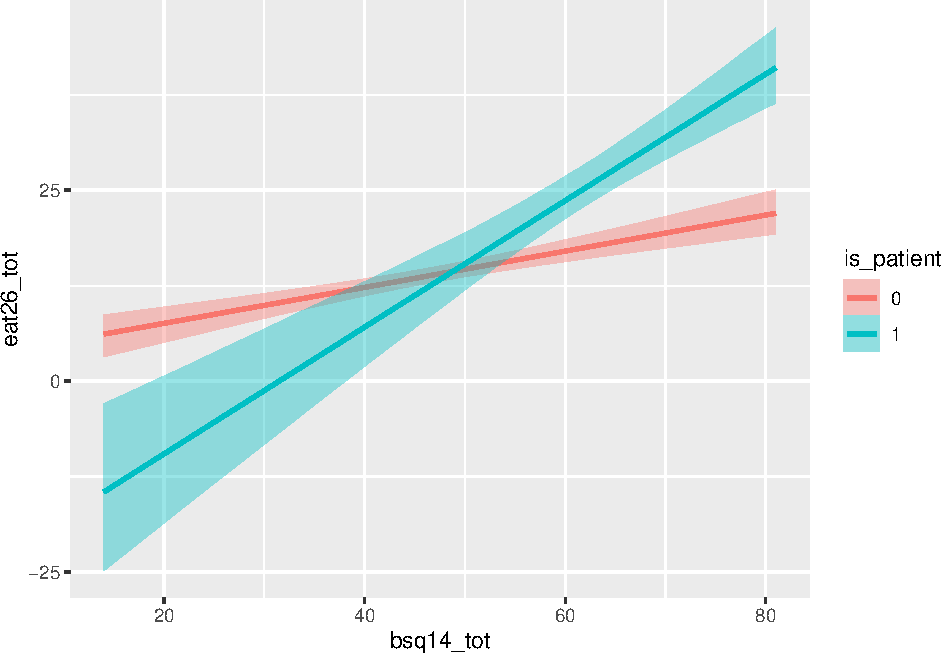
\includegraphics{050_quest_groups_files/figure-latex/unnamed-chunk-2-15.pdf}

\begin{Shaded}
\begin{Highlighting}[]
\FunctionTok{hist}\NormalTok{(dat}\SpecialCharTok{$}\NormalTok{bmi)}
\end{Highlighting}
\end{Shaded}

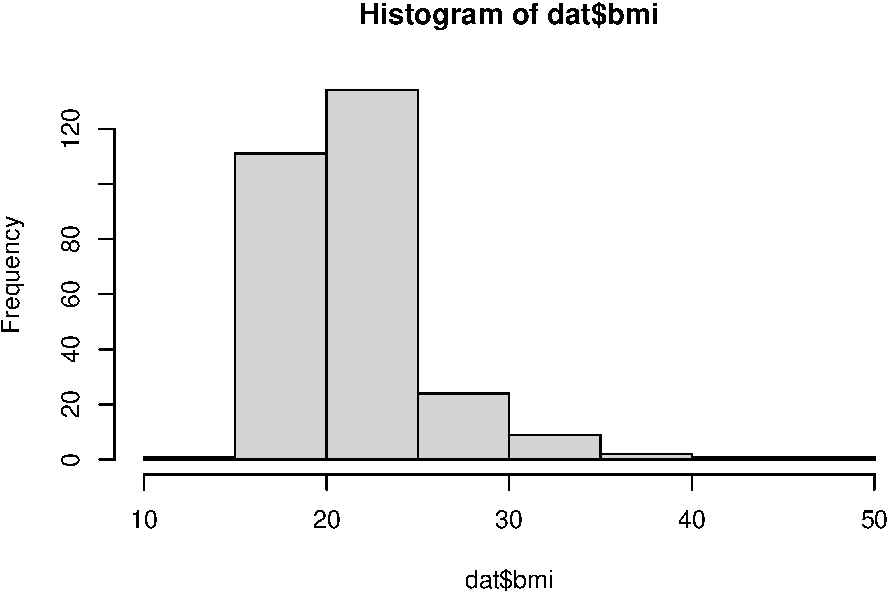
\includegraphics{050_quest_groups_files/figure-latex/unnamed-chunk-2-16.pdf}

\begin{Shaded}
\begin{Highlighting}[]
\NormalTok{dat}\SpecialCharTok{$}\NormalTok{bmi\_cat }\OtherTok{\textless{}{-}} \FunctionTok{cut}\NormalTok{(dat}\SpecialCharTok{$}\NormalTok{bmi, }\AttributeTok{breaks =} \FunctionTok{c}\NormalTok{(}\DecValTok{0}\NormalTok{, }\FloatTok{18.5}\NormalTok{, }\FloatTok{24.9}\NormalTok{, }\FloatTok{29.9}\NormalTok{, }\DecValTok{100}\NormalTok{))}
\FunctionTok{summary}\NormalTok{(dat}\SpecialCharTok{$}\NormalTok{bmi\_cat)}
\end{Highlighting}
\end{Shaded}

\begin{verbatim}
##    (0,18.5] (18.5,24.9] (24.9,29.9]  (29.9,100]        NA's 
##          41         200          29          13           1
\end{verbatim}

\begin{Shaded}
\begin{Highlighting}[]
\NormalTok{dat}\SpecialCharTok{$}\NormalTok{mps }\OtherTok{\textless{}{-}}\NormalTok{ dat}\SpecialCharTok{$}\NormalTok{mps\_ps }\SpecialCharTok{+}\NormalTok{ dat}\SpecialCharTok{$}\NormalTok{mps\_o }\SpecialCharTok{+}\NormalTok{ dat}\SpecialCharTok{$}\NormalTok{mps\_cmd }\SpecialCharTok{+}\NormalTok{ dat}\SpecialCharTok{$}\NormalTok{mps\_pepc}

\NormalTok{fm2 }\OtherTok{\textless{}{-}} \FunctionTok{brm}\NormalTok{(}
\NormalTok{  eat26\_tot }\SpecialCharTok{\textasciitilde{}}\NormalTok{ mps }\SpecialCharTok{*}\NormalTok{ (sex }\SpecialCharTok{+}\NormalTok{ is\_patient) }\SpecialCharTok{+}\NormalTok{ age }\SpecialCharTok{+}\NormalTok{ bmi,}
  \AttributeTok{data =}\NormalTok{ dat, }
  \CommentTok{\# prior = prior\_ma,}
  \AttributeTok{family =} \FunctionTok{skew\_normal}\NormalTok{(),}
  \AttributeTok{control =} \FunctionTok{list}\NormalTok{(}\AttributeTok{adapt\_delta =} \FloatTok{0.98}\NormalTok{),}
  \AttributeTok{iter =} \DecValTok{4000}\NormalTok{,}
  \AttributeTok{cores =} \DecValTok{6}\NormalTok{,}
  \AttributeTok{backend =} \StringTok{"cmdstan"}
\NormalTok{)}
\end{Highlighting}
\end{Shaded}

\begin{verbatim}
## Warning: Rows containing NAs were excluded from the model.
\end{verbatim}

\begin{verbatim}
## Start sampling
\end{verbatim}

\begin{verbatim}
## Running MCMC with 4 chains, at most 6 in parallel...
\end{verbatim}

\begin{verbatim}
## Chain 1 Rejecting initial value:
\end{verbatim}

\begin{verbatim}
## Chain 1   Log probability evaluates to log(0), i.e. negative infinity.
\end{verbatim}

\begin{verbatim}
## Chain 1   Stan can't start sampling from this initial value.
\end{verbatim}

\begin{verbatim}
## Chain 1 Rejecting initial value:
\end{verbatim}

\begin{verbatim}
## Chain 1   Log probability evaluates to log(0), i.e. negative infinity.
\end{verbatim}

\begin{verbatim}
## Chain 1   Stan can't start sampling from this initial value.
\end{verbatim}

\begin{verbatim}
## Chain 1 Rejecting initial value:
\end{verbatim}

\begin{verbatim}
## Chain 1   Log probability evaluates to log(0), i.e. negative infinity.
\end{verbatim}

\begin{verbatim}
## Chain 1   Stan can't start sampling from this initial value.
\end{verbatim}

\begin{verbatim}
## Chain 1 Rejecting initial value:
\end{verbatim}

\begin{verbatim}
## Chain 1   Log probability evaluates to log(0), i.e. negative infinity.
\end{verbatim}

\begin{verbatim}
## Chain 1   Stan can't start sampling from this initial value.
\end{verbatim}

\begin{verbatim}
## Chain 1 Iteration:    1 / 4000 [  0%]  (Warmup)
\end{verbatim}

\begin{verbatim}
## Chain 2 Rejecting initial value:
\end{verbatim}

\begin{verbatim}
## Chain 2   Log probability evaluates to log(0), i.e. negative infinity.
\end{verbatim}

\begin{verbatim}
## Chain 2   Stan can't start sampling from this initial value.
\end{verbatim}

\begin{verbatim}
## Chain 2 Rejecting initial value:
\end{verbatim}

\begin{verbatim}
## Chain 2   Log probability evaluates to log(0), i.e. negative infinity.
\end{verbatim}

\begin{verbatim}
## Chain 2   Stan can't start sampling from this initial value.
\end{verbatim}

\begin{verbatim}
## Chain 2 Rejecting initial value:
\end{verbatim}

\begin{verbatim}
## Chain 2   Log probability evaluates to log(0), i.e. negative infinity.
\end{verbatim}

\begin{verbatim}
## Chain 2   Stan can't start sampling from this initial value.
\end{verbatim}

\begin{verbatim}
## Chain 2 Iteration:    1 / 4000 [  0%]  (Warmup) 
## Chain 3 Iteration:    1 / 4000 [  0%]  (Warmup)
\end{verbatim}

\begin{verbatim}
## Chain 4 Rejecting initial value:
\end{verbatim}

\begin{verbatim}
## Chain 4   Log probability evaluates to log(0), i.e. negative infinity.
\end{verbatim}

\begin{verbatim}
## Chain 4   Stan can't start sampling from this initial value.
\end{verbatim}

\begin{verbatim}
## Chain 4 Rejecting initial value:
\end{verbatim}

\begin{verbatim}
## Chain 4   Log probability evaluates to log(0), i.e. negative infinity.
\end{verbatim}

\begin{verbatim}
## Chain 4   Stan can't start sampling from this initial value.
\end{verbatim}

\begin{verbatim}
## Chain 4 Rejecting initial value:
\end{verbatim}

\begin{verbatim}
## Chain 4   Log probability evaluates to log(0), i.e. negative infinity.
\end{verbatim}

\begin{verbatim}
## Chain 4   Stan can't start sampling from this initial value.
\end{verbatim}

\begin{verbatim}
## Chain 4 Iteration:    1 / 4000 [  0%]  (Warmup) 
## Chain 1 Iteration:  100 / 4000 [  2%]  (Warmup) 
## Chain 3 Iteration:  100 / 4000 [  2%]  (Warmup) 
## Chain 1 Iteration:  200 / 4000 [  5%]  (Warmup) 
## Chain 2 Iteration:  100 / 4000 [  2%]  (Warmup) 
## Chain 1 Iteration:  300 / 4000 [  7%]  (Warmup) 
## Chain 3 Iteration:  200 / 4000 [  5%]  (Warmup) 
## Chain 4 Iteration:  100 / 4000 [  2%]  (Warmup) 
## Chain 2 Iteration:  200 / 4000 [  5%]  (Warmup) 
## Chain 1 Iteration:  400 / 4000 [ 10%]  (Warmup) 
## Chain 2 Iteration:  300 / 4000 [  7%]  (Warmup) 
## Chain 3 Iteration:  300 / 4000 [  7%]  (Warmup) 
## Chain 3 Iteration:  400 / 4000 [ 10%]  (Warmup) 
## Chain 4 Iteration:  200 / 4000 [  5%]  (Warmup) 
## Chain 1 Iteration:  500 / 4000 [ 12%]  (Warmup) 
## Chain 2 Iteration:  400 / 4000 [ 10%]  (Warmup) 
## Chain 2 Iteration:  500 / 4000 [ 12%]  (Warmup) 
## Chain 4 Iteration:  300 / 4000 [  7%]  (Warmup) 
## Chain 1 Iteration:  600 / 4000 [ 15%]  (Warmup) 
## Chain 2 Iteration:  600 / 4000 [ 15%]  (Warmup) 
## Chain 3 Iteration:  500 / 4000 [ 12%]  (Warmup) 
## Chain 4 Iteration:  400 / 4000 [ 10%]  (Warmup) 
## Chain 1 Iteration:  700 / 4000 [ 17%]  (Warmup) 
## Chain 2 Iteration:  700 / 4000 [ 17%]  (Warmup) 
## Chain 3 Iteration:  600 / 4000 [ 15%]  (Warmup) 
## Chain 4 Iteration:  500 / 4000 [ 12%]  (Warmup) 
## Chain 1 Iteration:  800 / 4000 [ 20%]  (Warmup) 
## Chain 2 Iteration:  800 / 4000 [ 20%]  (Warmup) 
## Chain 3 Iteration:  700 / 4000 [ 17%]  (Warmup) 
## Chain 4 Iteration:  600 / 4000 [ 15%]  (Warmup) 
## Chain 2 Iteration:  900 / 4000 [ 22%]  (Warmup) 
## Chain 3 Iteration:  800 / 4000 [ 20%]  (Warmup) 
## Chain 1 Iteration:  900 / 4000 [ 22%]  (Warmup) 
## Chain 3 Iteration:  900 / 4000 [ 22%]  (Warmup) 
## Chain 4 Iteration:  700 / 4000 [ 17%]  (Warmup) 
## Chain 2 Iteration: 1000 / 4000 [ 25%]  (Warmup) 
## Chain 4 Iteration:  800 / 4000 [ 20%]  (Warmup) 
## Chain 1 Iteration: 1000 / 4000 [ 25%]  (Warmup) 
## Chain 3 Iteration: 1000 / 4000 [ 25%]  (Warmup) 
## Chain 2 Iteration: 1100 / 4000 [ 27%]  (Warmup) 
## Chain 1 Iteration: 1100 / 4000 [ 27%]  (Warmup) 
## Chain 2 Iteration: 1200 / 4000 [ 30%]  (Warmup) 
## Chain 3 Iteration: 1100 / 4000 [ 27%]  (Warmup) 
## Chain 1 Iteration: 1200 / 4000 [ 30%]  (Warmup) 
## Chain 3 Iteration: 1200 / 4000 [ 30%]  (Warmup) 
## Chain 4 Iteration:  900 / 4000 [ 22%]  (Warmup) 
## Chain 2 Iteration: 1300 / 4000 [ 32%]  (Warmup) 
## Chain 4 Iteration: 1000 / 4000 [ 25%]  (Warmup) 
## Chain 1 Iteration: 1300 / 4000 [ 32%]  (Warmup) 
## Chain 3 Iteration: 1300 / 4000 [ 32%]  (Warmup) 
## Chain 1 Iteration: 1400 / 4000 [ 35%]  (Warmup) 
## Chain 2 Iteration: 1400 / 4000 [ 35%]  (Warmup) 
## Chain 4 Iteration: 1100 / 4000 [ 27%]  (Warmup) 
## Chain 2 Iteration: 1500 / 4000 [ 37%]  (Warmup) 
## Chain 3 Iteration: 1400 / 4000 [ 35%]  (Warmup) 
## Chain 1 Iteration: 1500 / 4000 [ 37%]  (Warmup) 
## Chain 4 Iteration: 1200 / 4000 [ 30%]  (Warmup) 
## Chain 2 Iteration: 1600 / 4000 [ 40%]  (Warmup) 
## Chain 3 Iteration: 1500 / 4000 [ 37%]  (Warmup) 
## Chain 4 Iteration: 1300 / 4000 [ 32%]  (Warmup) 
## Chain 1 Iteration: 1600 / 4000 [ 40%]  (Warmup) 
## Chain 2 Iteration: 1700 / 4000 [ 42%]  (Warmup) 
## Chain 3 Iteration: 1600 / 4000 [ 40%]  (Warmup) 
## Chain 1 Iteration: 1700 / 4000 [ 42%]  (Warmup) 
## Chain 3 Iteration: 1700 / 4000 [ 42%]  (Warmup) 
## Chain 4 Iteration: 1400 / 4000 [ 35%]  (Warmup) 
## Chain 1 Iteration: 1800 / 4000 [ 45%]  (Warmup) 
## Chain 2 Iteration: 1800 / 4000 [ 45%]  (Warmup) 
## Chain 4 Iteration: 1500 / 4000 [ 37%]  (Warmup) 
## Chain 3 Iteration: 1800 / 4000 [ 45%]  (Warmup) 
## Chain 1 Iteration: 1900 / 4000 [ 47%]  (Warmup) 
## Chain 2 Iteration: 1900 / 4000 [ 47%]  (Warmup) 
## Chain 4 Iteration: 1600 / 4000 [ 40%]  (Warmup) 
## Chain 3 Iteration: 1900 / 4000 [ 47%]  (Warmup) 
## Chain 4 Iteration: 1700 / 4000 [ 42%]  (Warmup) 
## Chain 1 Iteration: 2000 / 4000 [ 50%]  (Warmup) 
## Chain 1 Iteration: 2001 / 4000 [ 50%]  (Sampling) 
## Chain 2 Iteration: 2000 / 4000 [ 50%]  (Warmup) 
## Chain 2 Iteration: 2001 / 4000 [ 50%]  (Sampling) 
## Chain 3 Iteration: 2000 / 4000 [ 50%]  (Warmup) 
## Chain 3 Iteration: 2001 / 4000 [ 50%]  (Sampling) 
## Chain 4 Iteration: 1800 / 4000 [ 45%]  (Warmup) 
## Chain 1 Iteration: 2100 / 4000 [ 52%]  (Sampling) 
## Chain 3 Iteration: 2100 / 4000 [ 52%]  (Sampling) 
## Chain 2 Iteration: 2100 / 4000 [ 52%]  (Sampling) 
## Chain 4 Iteration: 1900 / 4000 [ 47%]  (Warmup) 
## Chain 1 Iteration: 2200 / 4000 [ 55%]  (Sampling) 
## Chain 3 Iteration: 2200 / 4000 [ 55%]  (Sampling) 
## Chain 2 Iteration: 2200 / 4000 [ 55%]  (Sampling) 
## Chain 3 Iteration: 2300 / 4000 [ 57%]  (Sampling) 
## Chain 1 Iteration: 2300 / 4000 [ 57%]  (Sampling) 
## Chain 2 Iteration: 2300 / 4000 [ 57%]  (Sampling) 
## Chain 3 Iteration: 2400 / 4000 [ 60%]  (Sampling) 
## Chain 4 Iteration: 2000 / 4000 [ 50%]  (Warmup) 
## Chain 4 Iteration: 2001 / 4000 [ 50%]  (Sampling) 
## Chain 1 Iteration: 2400 / 4000 [ 60%]  (Sampling) 
## Chain 2 Iteration: 2400 / 4000 [ 60%]  (Sampling) 
## Chain 3 Iteration: 2500 / 4000 [ 62%]  (Sampling) 
## Chain 4 Iteration: 2100 / 4000 [ 52%]  (Sampling) 
## Chain 1 Iteration: 2500 / 4000 [ 62%]  (Sampling) 
## Chain 3 Iteration: 2600 / 4000 [ 65%]  (Sampling) 
## Chain 4 Iteration: 2200 / 4000 [ 55%]  (Sampling) 
## Chain 2 Iteration: 2500 / 4000 [ 62%]  (Sampling) 
## Chain 1 Iteration: 2600 / 4000 [ 65%]  (Sampling) 
## Chain 3 Iteration: 2700 / 4000 [ 67%]  (Sampling) 
## Chain 2 Iteration: 2600 / 4000 [ 65%]  (Sampling) 
## Chain 4 Iteration: 2300 / 4000 [ 57%]  (Sampling) 
## Chain 1 Iteration: 2700 / 4000 [ 67%]  (Sampling) 
## Chain 3 Iteration: 2800 / 4000 [ 70%]  (Sampling) 
## Chain 2 Iteration: 2700 / 4000 [ 67%]  (Sampling) 
## Chain 3 Iteration: 2900 / 4000 [ 72%]  (Sampling) 
## Chain 4 Iteration: 2400 / 4000 [ 60%]  (Sampling) 
## Chain 1 Iteration: 2800 / 4000 [ 70%]  (Sampling) 
## Chain 3 Iteration: 3000 / 4000 [ 75%]  (Sampling) 
## Chain 1 Iteration: 2900 / 4000 [ 72%]  (Sampling) 
## Chain 2 Iteration: 2800 / 4000 [ 70%]  (Sampling) 
## Chain 4 Iteration: 2500 / 4000 [ 62%]  (Sampling) 
## Chain 3 Iteration: 3100 / 4000 [ 77%]  (Sampling) 
## Chain 1 Iteration: 3000 / 4000 [ 75%]  (Sampling) 
## Chain 2 Iteration: 2900 / 4000 [ 72%]  (Sampling) 
## Chain 4 Iteration: 2600 / 4000 [ 65%]  (Sampling) 
## Chain 3 Iteration: 3200 / 4000 [ 80%]  (Sampling) 
## Chain 1 Iteration: 3100 / 4000 [ 77%]  (Sampling) 
## Chain 2 Iteration: 3000 / 4000 [ 75%]  (Sampling) 
## Chain 3 Iteration: 3300 / 4000 [ 82%]  (Sampling) 
## Chain 4 Iteration: 2700 / 4000 [ 67%]  (Sampling) 
## Chain 1 Iteration: 3200 / 4000 [ 80%]  (Sampling) 
## Chain 2 Iteration: 3100 / 4000 [ 77%]  (Sampling) 
## Chain 3 Iteration: 3400 / 4000 [ 85%]  (Sampling) 
## Chain 4 Iteration: 2800 / 4000 [ 70%]  (Sampling) 
## Chain 1 Iteration: 3300 / 4000 [ 82%]  (Sampling) 
## Chain 3 Iteration: 3500 / 4000 [ 87%]  (Sampling) 
## Chain 2 Iteration: 3200 / 4000 [ 80%]  (Sampling) 
## Chain 4 Iteration: 2900 / 4000 [ 72%]  (Sampling) 
## Chain 1 Iteration: 3400 / 4000 [ 85%]  (Sampling) 
## Chain 3 Iteration: 3600 / 4000 [ 90%]  (Sampling) 
## Chain 2 Iteration: 3300 / 4000 [ 82%]  (Sampling) 
## Chain 3 Iteration: 3700 / 4000 [ 92%]  (Sampling) 
## Chain 4 Iteration: 3000 / 4000 [ 75%]  (Sampling) 
## Chain 1 Iteration: 3500 / 4000 [ 87%]  (Sampling) 
## Chain 2 Iteration: 3400 / 4000 [ 85%]  (Sampling) 
## Chain 3 Iteration: 3800 / 4000 [ 95%]  (Sampling) 
## Chain 4 Iteration: 3100 / 4000 [ 77%]  (Sampling) 
## Chain 1 Iteration: 3600 / 4000 [ 90%]  (Sampling) 
## Chain 3 Iteration: 3900 / 4000 [ 97%]  (Sampling) 
## Chain 2 Iteration: 3500 / 4000 [ 87%]  (Sampling) 
## Chain 4 Iteration: 3200 / 4000 [ 80%]  (Sampling) 
## Chain 1 Iteration: 3700 / 4000 [ 92%]  (Sampling) 
## Chain 3 Iteration: 4000 / 4000 [100%]  (Sampling) 
## Chain 3 finished in 8.6 seconds.
## Chain 2 Iteration: 3600 / 4000 [ 90%]  (Sampling) 
## Chain 1 Iteration: 3800 / 4000 [ 95%]  (Sampling) 
## Chain 4 Iteration: 3300 / 4000 [ 82%]  (Sampling) 
## Chain 2 Iteration: 3700 / 4000 [ 92%]  (Sampling) 
## Chain 1 Iteration: 3900 / 4000 [ 97%]  (Sampling) 
## Chain 4 Iteration: 3400 / 4000 [ 85%]  (Sampling) 
## Chain 2 Iteration: 3800 / 4000 [ 95%]  (Sampling) 
## Chain 1 Iteration: 4000 / 4000 [100%]  (Sampling) 
## Chain 1 finished in 9.3 seconds.
## Chain 4 Iteration: 3500 / 4000 [ 87%]  (Sampling) 
## Chain 2 Iteration: 3900 / 4000 [ 97%]  (Sampling) 
## Chain 4 Iteration: 3600 / 4000 [ 90%]  (Sampling) 
## Chain 2 Iteration: 4000 / 4000 [100%]  (Sampling) 
## Chain 2 finished in 9.7 seconds.
## Chain 4 Iteration: 3700 / 4000 [ 92%]  (Sampling) 
## Chain 4 Iteration: 3800 / 4000 [ 95%]  (Sampling) 
## Chain 4 Iteration: 3900 / 4000 [ 97%]  (Sampling) 
## Chain 4 Iteration: 4000 / 4000 [100%]  (Sampling) 
## Chain 4 finished in 10.5 seconds.
## 
## All 4 chains finished successfully.
## Mean chain execution time: 9.5 seconds.
## Total execution time: 10.6 seconds.
\end{verbatim}

\begin{Shaded}
\begin{Highlighting}[]
\FunctionTok{summary}\NormalTok{(fm2)}
\end{Highlighting}
\end{Shaded}

\begin{verbatim}
##  Family: skew_normal 
##   Links: mu = identity; sigma = identity; alpha = identity 
## Formula: eat26_tot ~ mps * (sex + is_patient) + age + bmi 
##    Data: dat (Number of observations: 265) 
## Samples: 4 chains, each with iter = 4000; warmup = 2000; thin = 1;
##          total post-warmup samples = 8000
## 
## Population-Level Effects: 
##                 Estimate Est.Error l-95% CI u-95% CI Rhat Bulk_ESS Tail_ESS
## Intercept          12.03      3.90     4.33    19.79 1.00     5378     5298
## mps                 0.06      0.03     0.01     0.12 1.00     3554     5111
## sexMaschio          2.43      5.55    -9.05    12.84 1.00     3336     3882
## is_patient1        13.32      8.44    -2.63    30.87 1.00     3442     3702
## age                -0.07      0.08    -0.25     0.07 1.00     5837     4233
## bmi                -0.13      0.14    -0.41     0.13 1.00     5827     5784
## mps:sexMaschio     -0.03      0.05    -0.13     0.07 1.00     3255     4060
## mps:is_patient1    -0.06      0.07    -0.20     0.07 1.00     3566     3901
## 
## Family Specific Parameters: 
##       Estimate Est.Error l-95% CI u-95% CI Rhat Bulk_ESS Tail_ESS
## sigma     9.23      0.42     8.43    10.11 1.00     4674     4773
## alpha     9.31      2.28     5.53    14.25 1.00     3957     4824
## 
## Samples were drawn using sample(hmc). For each parameter, Bulk_ESS
## and Tail_ESS are effective sample size measures, and Rhat is the potential
## scale reduction factor on split chains (at convergence, Rhat = 1).
\end{verbatim}

\begin{Shaded}
\begin{Highlighting}[]
\FunctionTok{plot}\NormalTok{(}\FunctionTok{conditional\_effects}\NormalTok{(fm2, }\StringTok{"mps"}\NormalTok{))}
\end{Highlighting}
\end{Shaded}

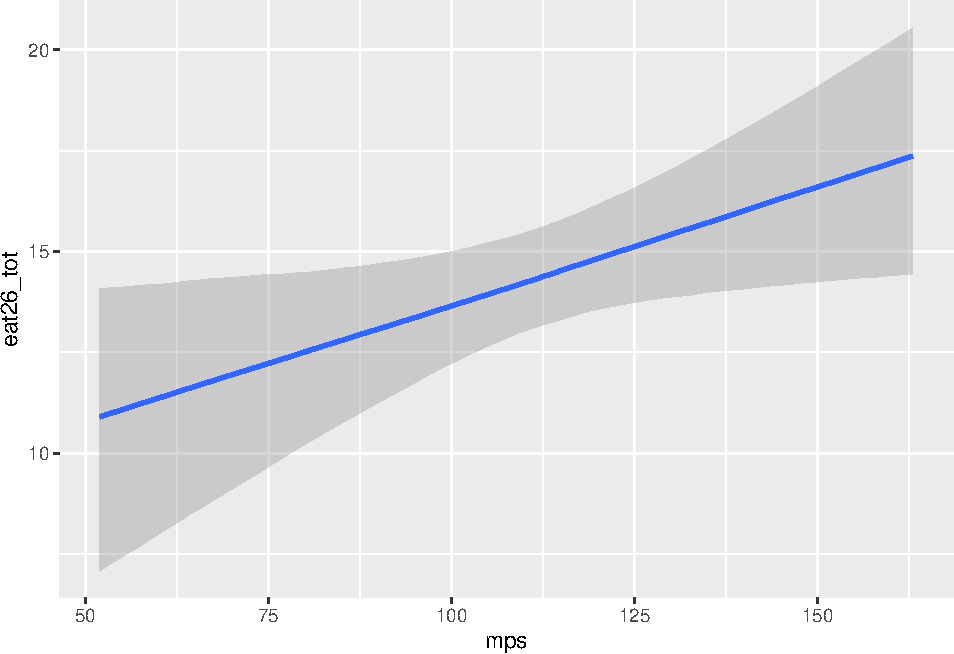
\includegraphics{050_quest_groups_files/figure-latex/unnamed-chunk-2-17.pdf}

\begin{Shaded}
\begin{Highlighting}[]
\NormalTok{fm3 }\OtherTok{\textless{}{-}} \FunctionTok{brm}\NormalTok{(}
\NormalTok{  eat26\_tot }\SpecialCharTok{\textasciitilde{}}\NormalTok{ sias }\SpecialCharTok{*}\NormalTok{ (sex }\SpecialCharTok{+}\NormalTok{ is\_patient) }\SpecialCharTok{+}\NormalTok{ age }\SpecialCharTok{+}\NormalTok{ bmi,}
  \AttributeTok{data =}\NormalTok{ dat, }
  \CommentTok{\# prior = prior\_ma,}
  \AttributeTok{family =} \FunctionTok{skew\_normal}\NormalTok{(),}
  \AttributeTok{control =} \FunctionTok{list}\NormalTok{(}\AttributeTok{adapt\_delta =} \FloatTok{0.98}\NormalTok{),}
  \AttributeTok{iter =} \DecValTok{4000}\NormalTok{,}
  \AttributeTok{cores =} \DecValTok{6}\NormalTok{,}
  \AttributeTok{backend =} \StringTok{"cmdstan"}
\NormalTok{)}
\end{Highlighting}
\end{Shaded}

\begin{verbatim}
## Warning: Rows containing NAs were excluded from the model.
\end{verbatim}

\begin{verbatim}
## Start sampling
\end{verbatim}

\begin{verbatim}
## Running MCMC with 4 chains, at most 6 in parallel...
\end{verbatim}

\begin{verbatim}
## Chain 1 Rejecting initial value:
\end{verbatim}

\begin{verbatim}
## Chain 1   Log probability evaluates to log(0), i.e. negative infinity.
\end{verbatim}

\begin{verbatim}
## Chain 1   Stan can't start sampling from this initial value.
\end{verbatim}

\begin{verbatim}
## Chain 1 Rejecting initial value:
\end{verbatim}

\begin{verbatim}
## Chain 1   Log probability evaluates to log(0), i.e. negative infinity.
\end{verbatim}

\begin{verbatim}
## Chain 1   Stan can't start sampling from this initial value.
\end{verbatim}

\begin{verbatim}
## Chain 1 Iteration:    1 / 4000 [  0%]  (Warmup) 
## Chain 2 Iteration:    1 / 4000 [  0%]  (Warmup)
\end{verbatim}

\begin{verbatim}
## Chain 3 Rejecting initial value:
\end{verbatim}

\begin{verbatim}
## Chain 3   Log probability evaluates to log(0), i.e. negative infinity.
\end{verbatim}

\begin{verbatim}
## Chain 3   Stan can't start sampling from this initial value.
\end{verbatim}

\begin{verbatim}
## Chain 3 Iteration:    1 / 4000 [  0%]  (Warmup)
\end{verbatim}

\begin{verbatim}
## Chain 4 Rejecting initial value:
\end{verbatim}

\begin{verbatim}
## Chain 4   Log probability evaluates to log(0), i.e. negative infinity.
\end{verbatim}

\begin{verbatim}
## Chain 4   Stan can't start sampling from this initial value.
\end{verbatim}

\begin{verbatim}
## Chain 4 Rejecting initial value:
\end{verbatim}

\begin{verbatim}
## Chain 4   Log probability evaluates to log(0), i.e. negative infinity.
\end{verbatim}

\begin{verbatim}
## Chain 4   Stan can't start sampling from this initial value.
\end{verbatim}

\begin{verbatim}
## Chain 4 Iteration:    1 / 4000 [  0%]  (Warmup) 
## Chain 1 Iteration:  100 / 4000 [  2%]  (Warmup) 
## Chain 2 Iteration:  100 / 4000 [  2%]  (Warmup) 
## Chain 4 Iteration:  100 / 4000 [  2%]  (Warmup) 
## Chain 1 Iteration:  200 / 4000 [  5%]  (Warmup) 
## Chain 2 Iteration:  200 / 4000 [  5%]  (Warmup) 
## Chain 3 Iteration:  100 / 4000 [  2%]  (Warmup) 
## Chain 4 Iteration:  200 / 4000 [  5%]  (Warmup) 
## Chain 1 Iteration:  300 / 4000 [  7%]  (Warmup) 
## Chain 3 Iteration:  200 / 4000 [  5%]  (Warmup) 
## Chain 4 Iteration:  300 / 4000 [  7%]  (Warmup) 
## Chain 2 Iteration:  300 / 4000 [  7%]  (Warmup) 
## Chain 4 Iteration:  400 / 4000 [ 10%]  (Warmup) 
## Chain 1 Iteration:  400 / 4000 [ 10%]  (Warmup) 
## Chain 2 Iteration:  400 / 4000 [ 10%]  (Warmup) 
## Chain 3 Iteration:  300 / 4000 [  7%]  (Warmup) 
## Chain 1 Iteration:  500 / 4000 [ 12%]  (Warmup) 
## Chain 3 Iteration:  400 / 4000 [ 10%]  (Warmup) 
## Chain 4 Iteration:  500 / 4000 [ 12%]  (Warmup) 
## Chain 1 Iteration:  600 / 4000 [ 15%]  (Warmup) 
## Chain 2 Iteration:  500 / 4000 [ 12%]  (Warmup) 
## Chain 3 Iteration:  500 / 4000 [ 12%]  (Warmup) 
## Chain 3 Iteration:  600 / 4000 [ 15%]  (Warmup) 
## Chain 4 Iteration:  600 / 4000 [ 15%]  (Warmup) 
## Chain 1 Iteration:  700 / 4000 [ 17%]  (Warmup) 
## Chain 2 Iteration:  600 / 4000 [ 15%]  (Warmup) 
## Chain 4 Iteration:  700 / 4000 [ 17%]  (Warmup) 
## Chain 1 Iteration:  800 / 4000 [ 20%]  (Warmup) 
## Chain 2 Iteration:  700 / 4000 [ 17%]  (Warmup) 
## Chain 3 Iteration:  700 / 4000 [ 17%]  (Warmup) 
## Chain 4 Iteration:  800 / 4000 [ 20%]  (Warmup) 
## Chain 1 Iteration:  900 / 4000 [ 22%]  (Warmup) 
## Chain 2 Iteration:  800 / 4000 [ 20%]  (Warmup) 
## Chain 3 Iteration:  800 / 4000 [ 20%]  (Warmup) 
## Chain 1 Iteration: 1000 / 4000 [ 25%]  (Warmup) 
## Chain 4 Iteration:  900 / 4000 [ 22%]  (Warmup) 
## Chain 1 Iteration: 1100 / 4000 [ 27%]  (Warmup) 
## Chain 2 Iteration:  900 / 4000 [ 22%]  (Warmup) 
## Chain 3 Iteration:  900 / 4000 [ 22%]  (Warmup) 
## Chain 4 Iteration: 1000 / 4000 [ 25%]  (Warmup) 
## Chain 4 Iteration: 1100 / 4000 [ 27%]  (Warmup) 
## Chain 1 Iteration: 1200 / 4000 [ 30%]  (Warmup) 
## Chain 2 Iteration: 1000 / 4000 [ 25%]  (Warmup) 
## Chain 3 Iteration: 1000 / 4000 [ 25%]  (Warmup) 
## Chain 1 Iteration: 1300 / 4000 [ 32%]  (Warmup) 
## Chain 2 Iteration: 1100 / 4000 [ 27%]  (Warmup) 
## Chain 3 Iteration: 1100 / 4000 [ 27%]  (Warmup) 
## Chain 4 Iteration: 1200 / 4000 [ 30%]  (Warmup) 
## Chain 1 Iteration: 1400 / 4000 [ 35%]  (Warmup) 
## Chain 2 Iteration: 1200 / 4000 [ 30%]  (Warmup) 
## Chain 3 Iteration: 1200 / 4000 [ 30%]  (Warmup) 
## Chain 4 Iteration: 1300 / 4000 [ 32%]  (Warmup) 
## Chain 1 Iteration: 1500 / 4000 [ 37%]  (Warmup) 
## Chain 2 Iteration: 1300 / 4000 [ 32%]  (Warmup) 
## Chain 3 Iteration: 1300 / 4000 [ 32%]  (Warmup) 
## Chain 4 Iteration: 1400 / 4000 [ 35%]  (Warmup) 
## Chain 1 Iteration: 1600 / 4000 [ 40%]  (Warmup) 
## Chain 4 Iteration: 1500 / 4000 [ 37%]  (Warmup) 
## Chain 2 Iteration: 1400 / 4000 [ 35%]  (Warmup) 
## Chain 3 Iteration: 1400 / 4000 [ 35%]  (Warmup) 
## Chain 1 Iteration: 1700 / 4000 [ 42%]  (Warmup) 
## Chain 2 Iteration: 1500 / 4000 [ 37%]  (Warmup) 
## Chain 3 Iteration: 1500 / 4000 [ 37%]  (Warmup) 
## Chain 4 Iteration: 1600 / 4000 [ 40%]  (Warmup) 
## Chain 1 Iteration: 1800 / 4000 [ 45%]  (Warmup) 
## Chain 3 Iteration: 1600 / 4000 [ 40%]  (Warmup) 
## Chain 4 Iteration: 1700 / 4000 [ 42%]  (Warmup) 
## Chain 1 Iteration: 1900 / 4000 [ 47%]  (Warmup) 
## Chain 2 Iteration: 1600 / 4000 [ 40%]  (Warmup) 
## Chain 4 Iteration: 1800 / 4000 [ 45%]  (Warmup) 
## Chain 1 Iteration: 2000 / 4000 [ 50%]  (Warmup) 
## Chain 1 Iteration: 2001 / 4000 [ 50%]  (Sampling) 
## Chain 2 Iteration: 1700 / 4000 [ 42%]  (Warmup) 
## Chain 3 Iteration: 1700 / 4000 [ 42%]  (Warmup) 
## Chain 2 Iteration: 1800 / 4000 [ 45%]  (Warmup) 
## Chain 3 Iteration: 1800 / 4000 [ 45%]  (Warmup) 
## Chain 4 Iteration: 1900 / 4000 [ 47%]  (Warmup) 
## Chain 1 Iteration: 2100 / 4000 [ 52%]  (Sampling) 
## Chain 3 Iteration: 1900 / 4000 [ 47%]  (Warmup) 
## Chain 4 Iteration: 2000 / 4000 [ 50%]  (Warmup) 
## Chain 4 Iteration: 2001 / 4000 [ 50%]  (Sampling) 
## Chain 1 Iteration: 2200 / 4000 [ 55%]  (Sampling) 
## Chain 2 Iteration: 1900 / 4000 [ 47%]  (Warmup) 
## Chain 3 Iteration: 2000 / 4000 [ 50%]  (Warmup) 
## Chain 3 Iteration: 2001 / 4000 [ 50%]  (Sampling) 
## Chain 1 Iteration: 2300 / 4000 [ 57%]  (Sampling) 
## Chain 2 Iteration: 2000 / 4000 [ 50%]  (Warmup) 
## Chain 2 Iteration: 2001 / 4000 [ 50%]  (Sampling) 
## Chain 3 Iteration: 2100 / 4000 [ 52%]  (Sampling) 
## Chain 4 Iteration: 2100 / 4000 [ 52%]  (Sampling) 
## Chain 1 Iteration: 2400 / 4000 [ 60%]  (Sampling) 
## Chain 2 Iteration: 2100 / 4000 [ 52%]  (Sampling) 
## Chain 4 Iteration: 2200 / 4000 [ 55%]  (Sampling) 
## Chain 1 Iteration: 2500 / 4000 [ 62%]  (Sampling) 
## Chain 3 Iteration: 2200 / 4000 [ 55%]  (Sampling) 
## Chain 4 Iteration: 2300 / 4000 [ 57%]  (Sampling) 
## Chain 1 Iteration: 2600 / 4000 [ 65%]  (Sampling) 
## Chain 2 Iteration: 2200 / 4000 [ 55%]  (Sampling) 
## Chain 3 Iteration: 2300 / 4000 [ 57%]  (Sampling) 
## Chain 4 Iteration: 2400 / 4000 [ 60%]  (Sampling) 
## Chain 1 Iteration: 2700 / 4000 [ 67%]  (Sampling) 
## Chain 2 Iteration: 2300 / 4000 [ 57%]  (Sampling) 
## Chain 3 Iteration: 2400 / 4000 [ 60%]  (Sampling) 
## Chain 3 Iteration: 2500 / 4000 [ 62%]  (Sampling) 
## Chain 4 Iteration: 2500 / 4000 [ 62%]  (Sampling) 
## Chain 1 Iteration: 2800 / 4000 [ 70%]  (Sampling) 
## Chain 2 Iteration: 2400 / 4000 [ 60%]  (Sampling) 
## Chain 3 Iteration: 2600 / 4000 [ 65%]  (Sampling) 
## Chain 4 Iteration: 2600 / 4000 [ 65%]  (Sampling) 
## Chain 1 Iteration: 2900 / 4000 [ 72%]  (Sampling) 
## Chain 2 Iteration: 2500 / 4000 [ 62%]  (Sampling) 
## Chain 3 Iteration: 2700 / 4000 [ 67%]  (Sampling) 
## Chain 4 Iteration: 2700 / 4000 [ 67%]  (Sampling) 
## Chain 1 Iteration: 3000 / 4000 [ 75%]  (Sampling) 
## Chain 2 Iteration: 2600 / 4000 [ 65%]  (Sampling) 
## Chain 3 Iteration: 2800 / 4000 [ 70%]  (Sampling) 
## Chain 1 Iteration: 3100 / 4000 [ 77%]  (Sampling) 
## Chain 3 Iteration: 2900 / 4000 [ 72%]  (Sampling) 
## Chain 4 Iteration: 2800 / 4000 [ 70%]  (Sampling) 
## Chain 1 Iteration: 3200 / 4000 [ 80%]  (Sampling) 
## Chain 2 Iteration: 2700 / 4000 [ 67%]  (Sampling) 
## Chain 3 Iteration: 3000 / 4000 [ 75%]  (Sampling) 
## Chain 4 Iteration: 2900 / 4000 [ 72%]  (Sampling) 
## Chain 1 Iteration: 3300 / 4000 [ 82%]  (Sampling) 
## Chain 2 Iteration: 2800 / 4000 [ 70%]  (Sampling) 
## Chain 3 Iteration: 3100 / 4000 [ 77%]  (Sampling) 
## Chain 4 Iteration: 3000 / 4000 [ 75%]  (Sampling) 
## Chain 2 Iteration: 2900 / 4000 [ 72%]  (Sampling) 
## Chain 3 Iteration: 3200 / 4000 [ 80%]  (Sampling) 
## Chain 4 Iteration: 3100 / 4000 [ 77%]  (Sampling) 
## Chain 1 Iteration: 3400 / 4000 [ 85%]  (Sampling) 
## Chain 1 Iteration: 3500 / 4000 [ 87%]  (Sampling) 
## Chain 2 Iteration: 3000 / 4000 [ 75%]  (Sampling) 
## Chain 3 Iteration: 3300 / 4000 [ 82%]  (Sampling) 
## Chain 4 Iteration: 3200 / 4000 [ 80%]  (Sampling) 
## Chain 1 Iteration: 3600 / 4000 [ 90%]  (Sampling) 
## Chain 2 Iteration: 3100 / 4000 [ 77%]  (Sampling) 
## Chain 3 Iteration: 3400 / 4000 [ 85%]  (Sampling) 
## Chain 4 Iteration: 3300 / 4000 [ 82%]  (Sampling) 
## Chain 1 Iteration: 3700 / 4000 [ 92%]  (Sampling) 
## Chain 3 Iteration: 3500 / 4000 [ 87%]  (Sampling) 
## Chain 4 Iteration: 3400 / 4000 [ 85%]  (Sampling) 
## Chain 1 Iteration: 3800 / 4000 [ 95%]  (Sampling) 
## Chain 2 Iteration: 3200 / 4000 [ 80%]  (Sampling) 
## Chain 3 Iteration: 3600 / 4000 [ 90%]  (Sampling) 
## Chain 2 Iteration: 3300 / 4000 [ 82%]  (Sampling) 
## Chain 3 Iteration: 3700 / 4000 [ 92%]  (Sampling) 
## Chain 4 Iteration: 3500 / 4000 [ 87%]  (Sampling) 
## Chain 1 Iteration: 3900 / 4000 [ 97%]  (Sampling) 
## Chain 3 Iteration: 3800 / 4000 [ 95%]  (Sampling) 
## Chain 4 Iteration: 3600 / 4000 [ 90%]  (Sampling) 
## Chain 1 Iteration: 4000 / 4000 [100%]  (Sampling) 
## Chain 2 Iteration: 3400 / 4000 [ 85%]  (Sampling) 
## Chain 3 Iteration: 3900 / 4000 [ 97%]  (Sampling) 
## Chain 4 Iteration: 3700 / 4000 [ 92%]  (Sampling) 
## Chain 1 finished in 5.6 seconds.
## Chain 2 Iteration: 3500 / 4000 [ 87%]  (Sampling) 
## Chain 3 Iteration: 4000 / 4000 [100%]  (Sampling) 
## Chain 4 Iteration: 3800 / 4000 [ 95%]  (Sampling) 
## Chain 3 finished in 5.8 seconds.
## Chain 2 Iteration: 3600 / 4000 [ 90%]  (Sampling) 
## Chain 4 Iteration: 3900 / 4000 [ 97%]  (Sampling) 
## Chain 2 Iteration: 3700 / 4000 [ 92%]  (Sampling) 
## Chain 4 Iteration: 4000 / 4000 [100%]  (Sampling) 
## Chain 4 finished in 6.0 seconds.
## Chain 2 Iteration: 3800 / 4000 [ 95%]  (Sampling) 
## Chain 2 Iteration: 3900 / 4000 [ 97%]  (Sampling) 
## Chain 2 Iteration: 4000 / 4000 [100%]  (Sampling) 
## Chain 2 finished in 6.4 seconds.
## 
## All 4 chains finished successfully.
## Mean chain execution time: 6.0 seconds.
## Total execution time: 6.5 seconds.
\end{verbatim}

\begin{Shaded}
\begin{Highlighting}[]
\FunctionTok{summary}\NormalTok{(fm3)}
\end{Highlighting}
\end{Shaded}

\begin{verbatim}
##  Family: skew_normal 
##   Links: mu = identity; sigma = identity; alpha = identity 
## Formula: eat26_tot ~ sias * (sex + is_patient) + age + bmi 
##    Data: dat (Number of observations: 265) 
## Samples: 4 chains, each with iter = 4000; warmup = 2000; thin = 1;
##          total post-warmup samples = 8000
## 
## Population-Level Effects: 
##                  Estimate Est.Error l-95% CI u-95% CI Rhat Bulk_ESS Tail_ESS
## Intercept           19.18      3.05    13.26    25.28 1.00     6549     5615
## sias                 0.07      0.03     0.00     0.14 1.00     4963     4782
## sexMaschio           1.89      2.28    -2.93     6.17 1.00     4570     5485
## is_patient1         -4.70      5.61   -15.01     6.77 1.00     4155     4676
## age                 -0.10      0.08    -0.26     0.04 1.00     5871     4800
## bmi                 -0.24      0.13    -0.50     0.01 1.00     6467     5354
## sias:sexMaschio     -0.09      0.08    -0.25     0.05 1.00     4635     4910
## sias:is_patient1     0.34      0.16     0.01     0.64 1.00     4249     4796
## 
## Family Specific Parameters: 
##       Estimate Est.Error l-95% CI u-95% CI Rhat Bulk_ESS Tail_ESS
## sigma     9.16      0.41     8.40    10.03 1.00     5122     4906
## alpha    10.49      2.33     6.46    15.54 1.00     5268     5552
## 
## Samples were drawn using sample(hmc). For each parameter, Bulk_ESS
## and Tail_ESS are effective sample size measures, and Rhat is the potential
## scale reduction factor on split chains (at convergence, Rhat = 1).
\end{verbatim}

\begin{Shaded}
\begin{Highlighting}[]
\FunctionTok{plot}\NormalTok{(}\FunctionTok{conditional\_effects}\NormalTok{(fm3, }\StringTok{"sias:is\_patient"}\NormalTok{))}
\end{Highlighting}
\end{Shaded}

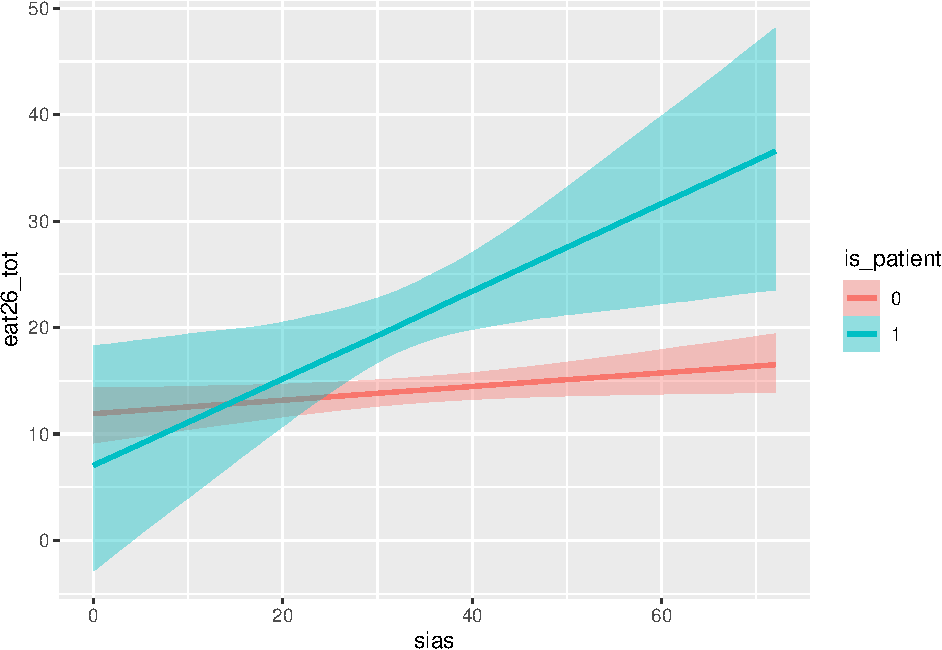
\includegraphics{050_quest_groups_files/figure-latex/unnamed-chunk-2-18.pdf}

\end{document}
